\begin{figure}
	\centering
	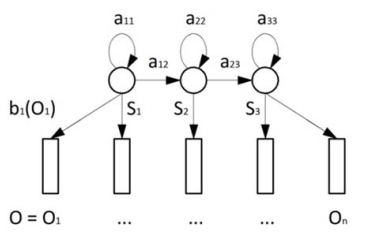
\includegraphics [width=.5\linewidth] {hmm}
	\caption{Топологія прихованих Марковських моделей з трьома станами}
	\label{img:hmm}
\end{figure}
\begin{figure}
	\centering
	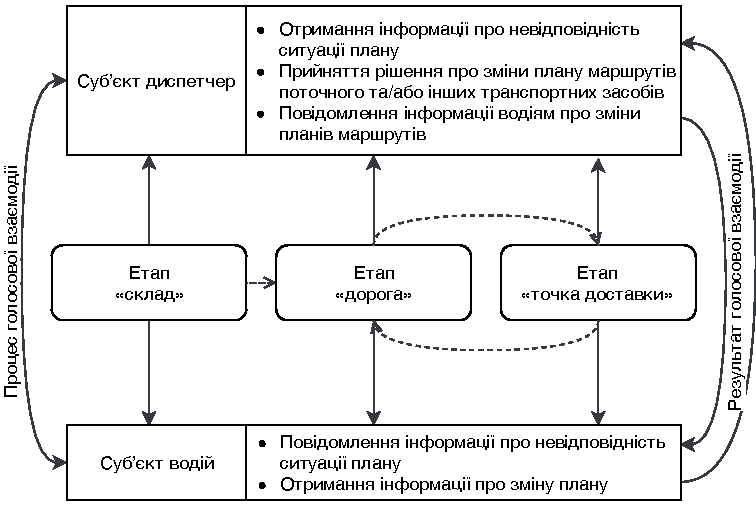
\includegraphics [width=\linewidth] {voice_interaction_schema}
	\caption{Схема голосової взаємодії субʼєктів дистрибуції}
	\label{img:voice_interaction_schema}
\end{figure}
\begin{figure}
	\centering
	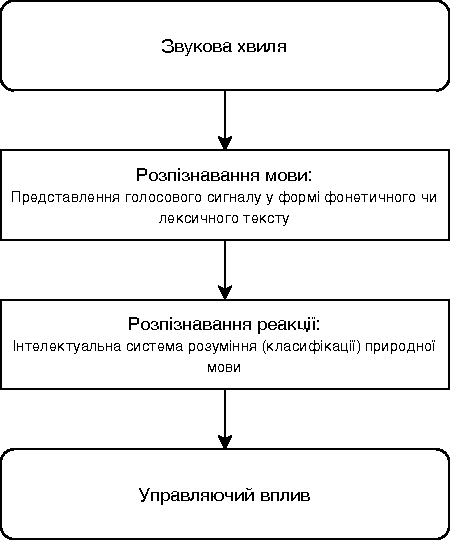
\includegraphics [width=.5\linewidth] {rgsu_concept}
	\caption{Схема узагальненої структури рефлекторних систем голосового управління}
	\label{img:rgsu_concept}
\end{figure}
\begin{figure}
	\centering
	
\includegraphics [width=1\linewidth] {01_simplest_positive_scenario}
	\caption{Найпростіше дерево сценаріїв}
	\label{img:01_simplest_positive_scenario}
\end{figure}
\begin{figure}
	\centering
	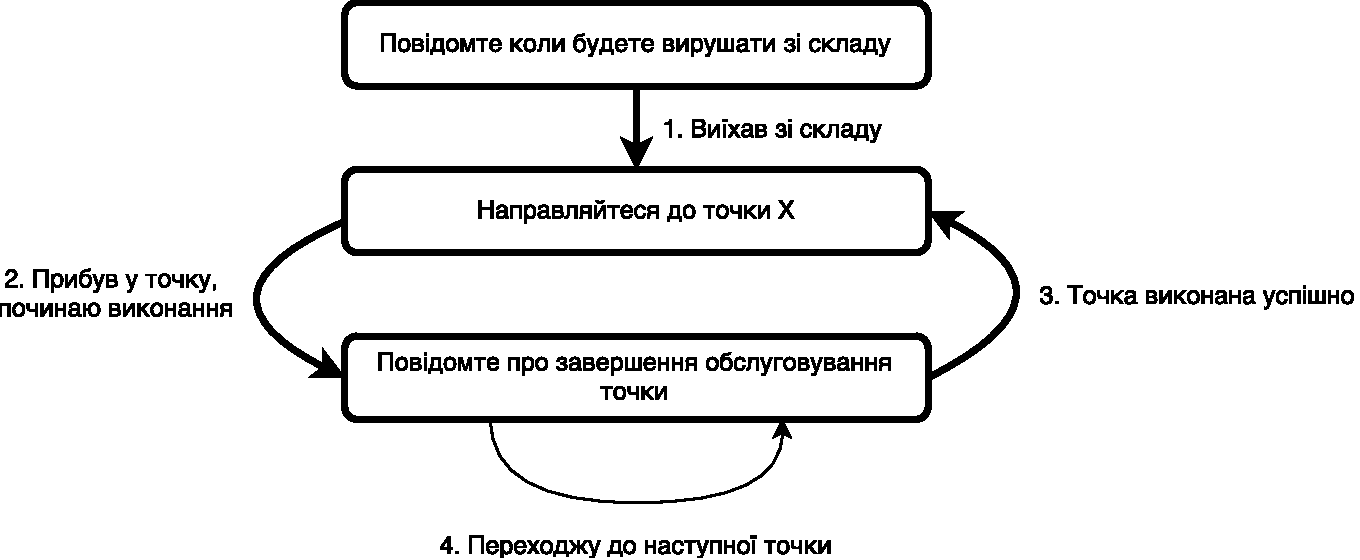
\includegraphics [width=1\linewidth] {02_simplest_positive_scenario_vertical}
	\caption{Вертикальний розподіл найпростішого дерева сценаріїв}
	\label{img:02_simplest_positive_scenario_vertical}
\end{figure}
\begin{figure}
	\centering
	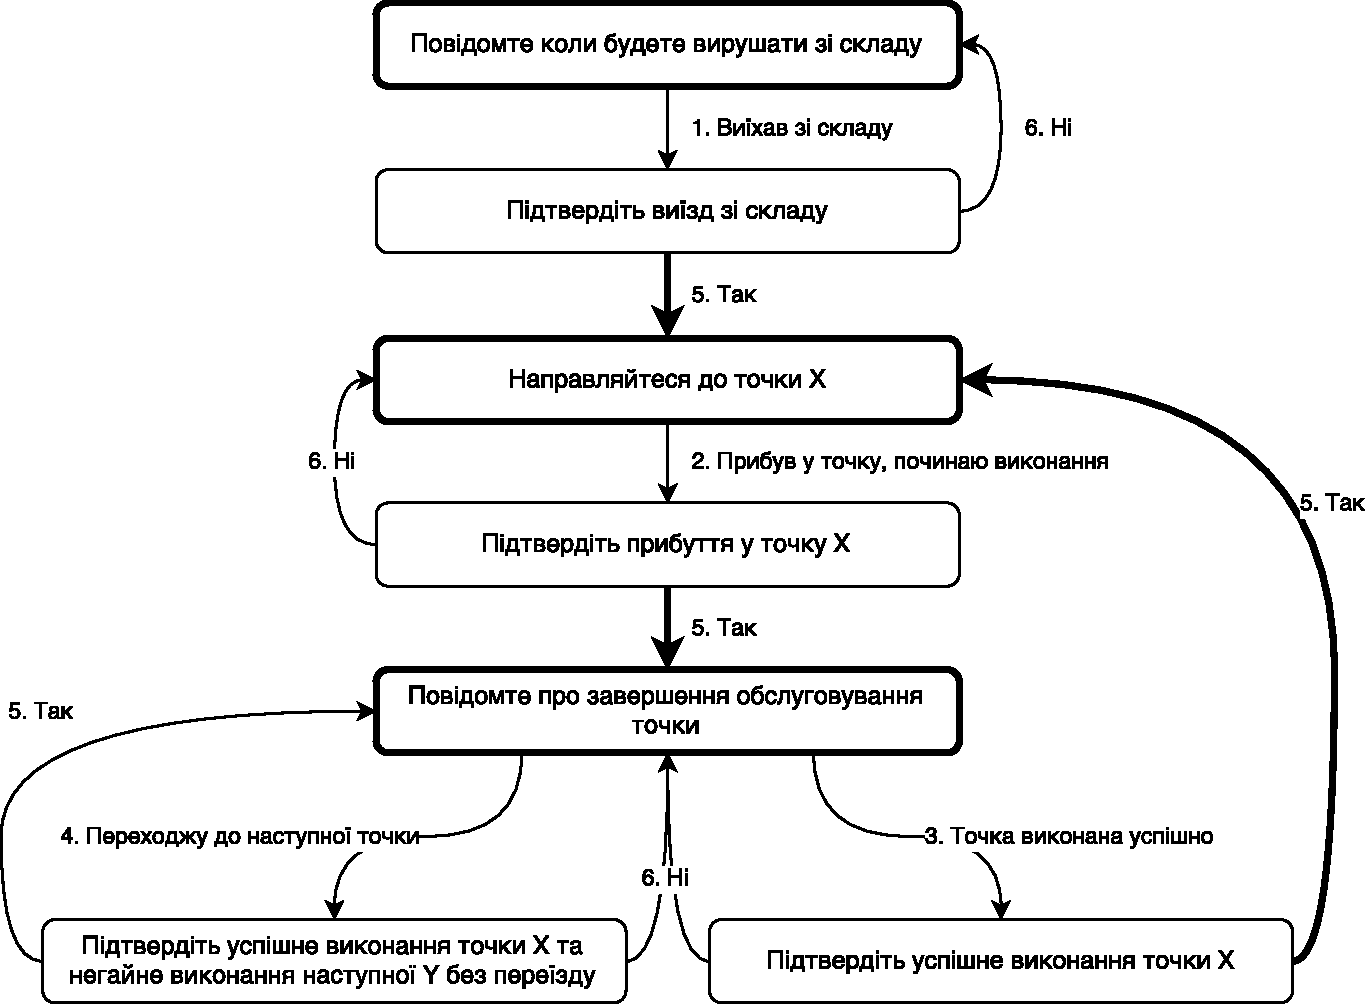
\includegraphics [width=1\linewidth] {03_positive_scenario_with_conformation}
	\caption{Позитивне дерево сценаріїв з підтвердженням}
	\label{img:03_positive_scenario_with_conformation}
\end{figure}
\begin{figure}
	\centering
	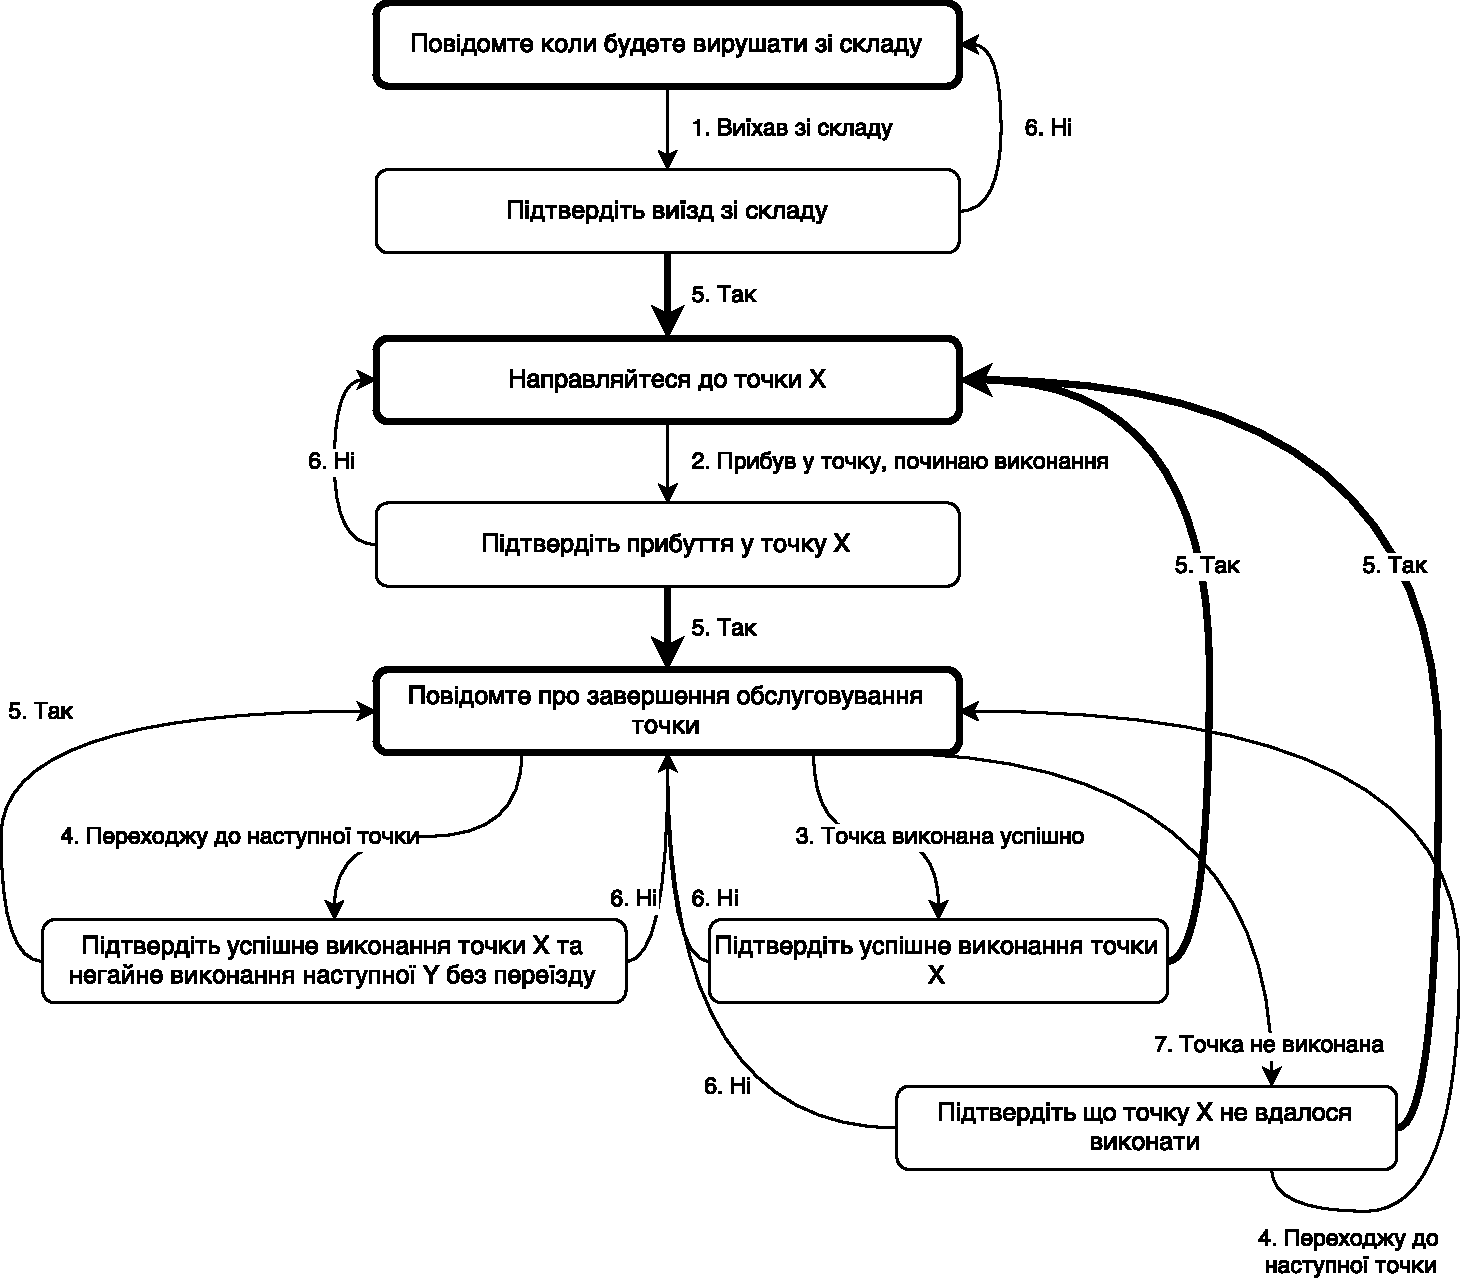
\includegraphics [width=1\linewidth] {04_first_negative_scenario_with_conformation}
	\caption{Перший варіант дерева сценаріїв з негативними інцидентами}
	\label{img:04_first_negative_scenario_with_conformation}
\end{figure}
\begin{figure}
	\centering
	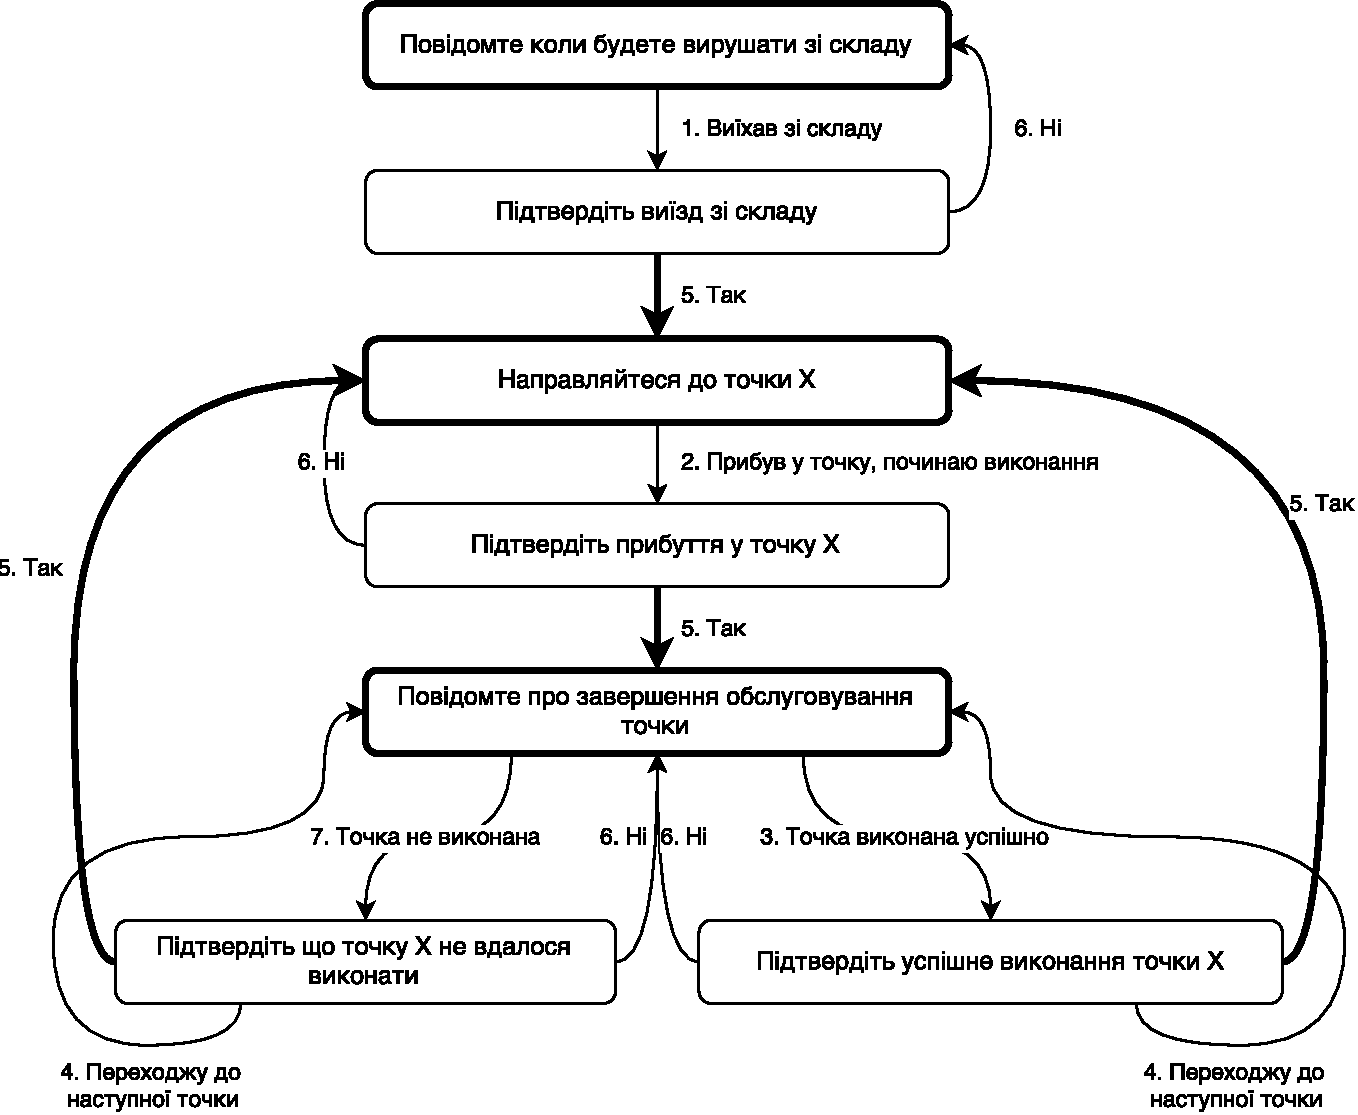
\includegraphics [width=1\linewidth] {05_simple_negative_scenario_with_conformation}
	\caption{Спрощений варіант дерева сценаріїв з негативними інцидентами}
	\label{img:05_simple_negative_scenario_with_conformation}
\end{figure}
\begin{figure}
	\centering
	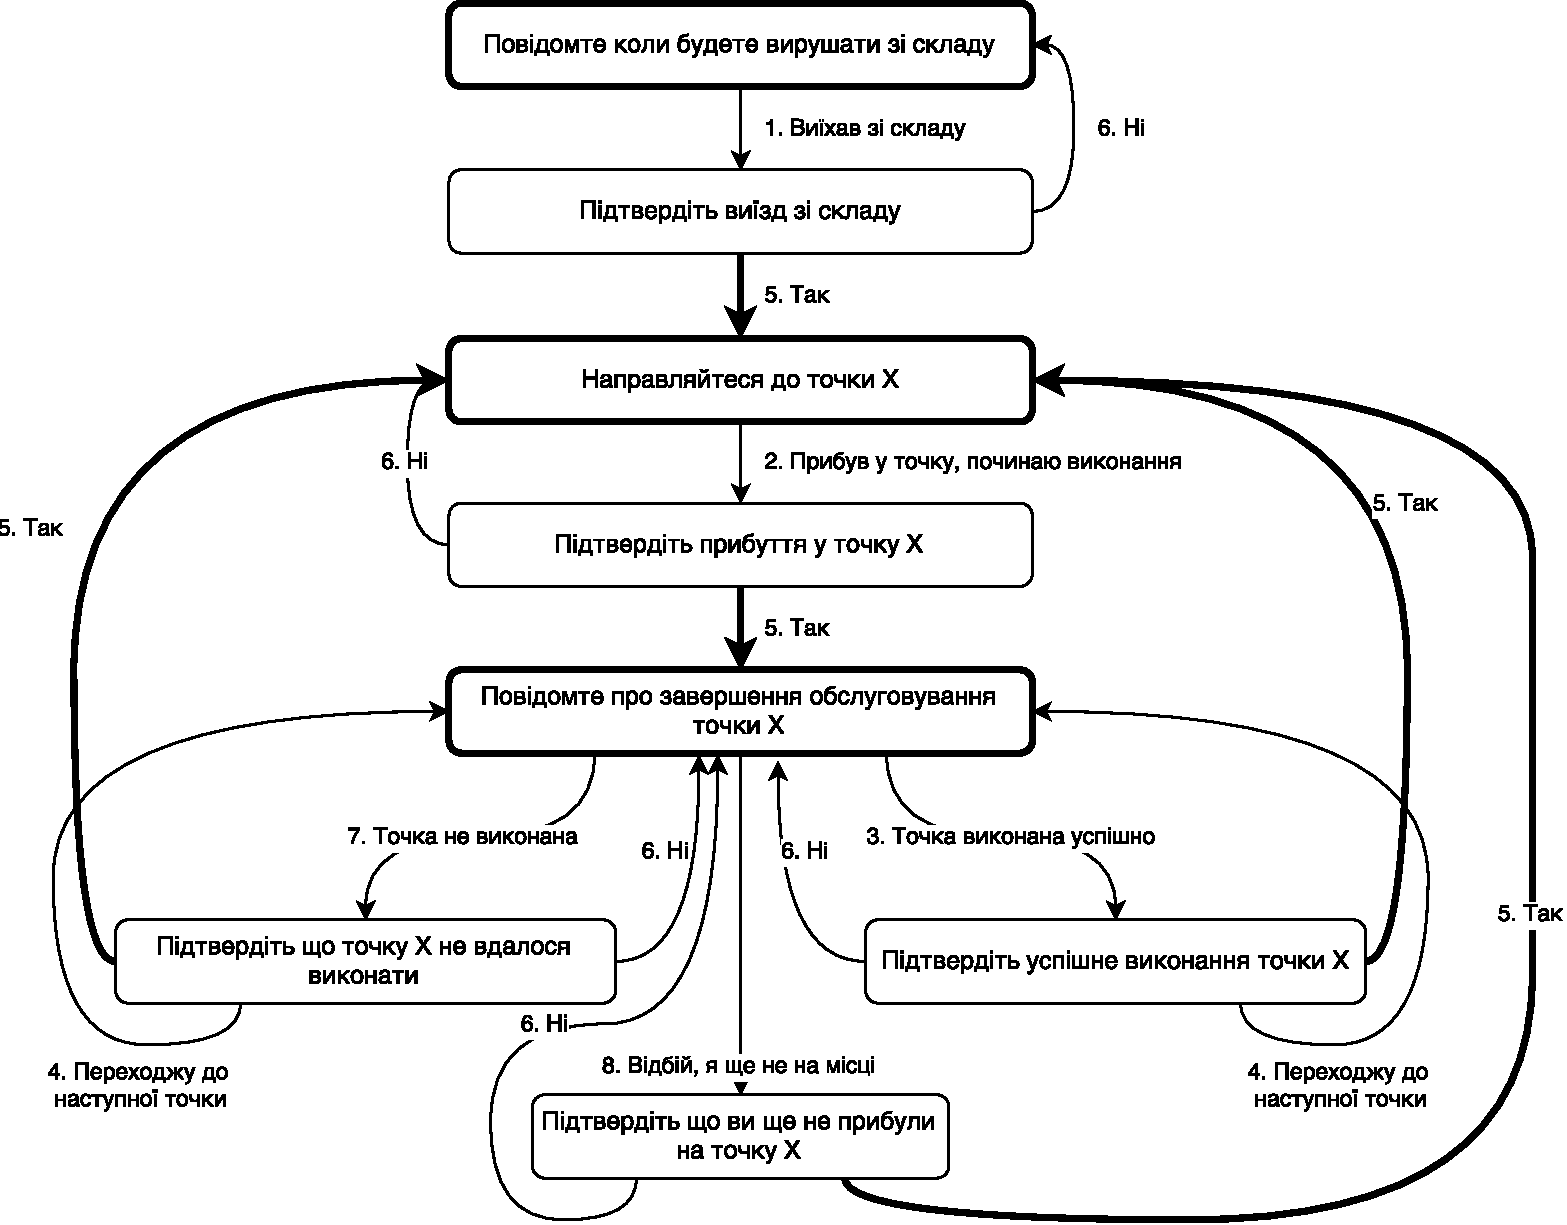
\includegraphics [width=1\linewidth] {06_simple_negative_scenario_with_rollback}
	\caption{Варіант дерева сценаріїв з негативними інцидентами та відбоєм}
	\label{img:06_simple_negative_scenario_with_rollback}
\end{figure}
\begin{figure}
	\centering
	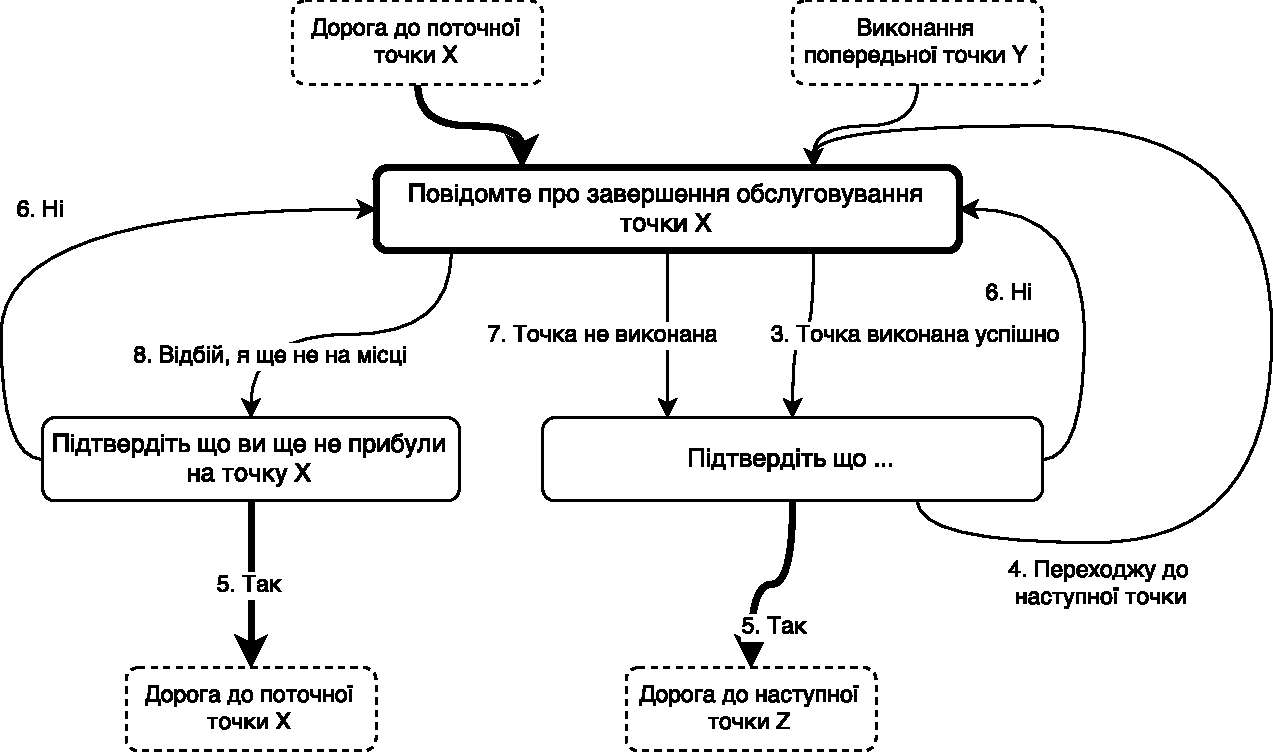
\includegraphics [width=1\linewidth] {07_simple_point_scenario}
	\caption{Частина дерева сценаріїв етапу <<точка доставки>>}
	\label{img:07_simple_point_scenario}
\end{figure}
\begin{figure}
	\centering
	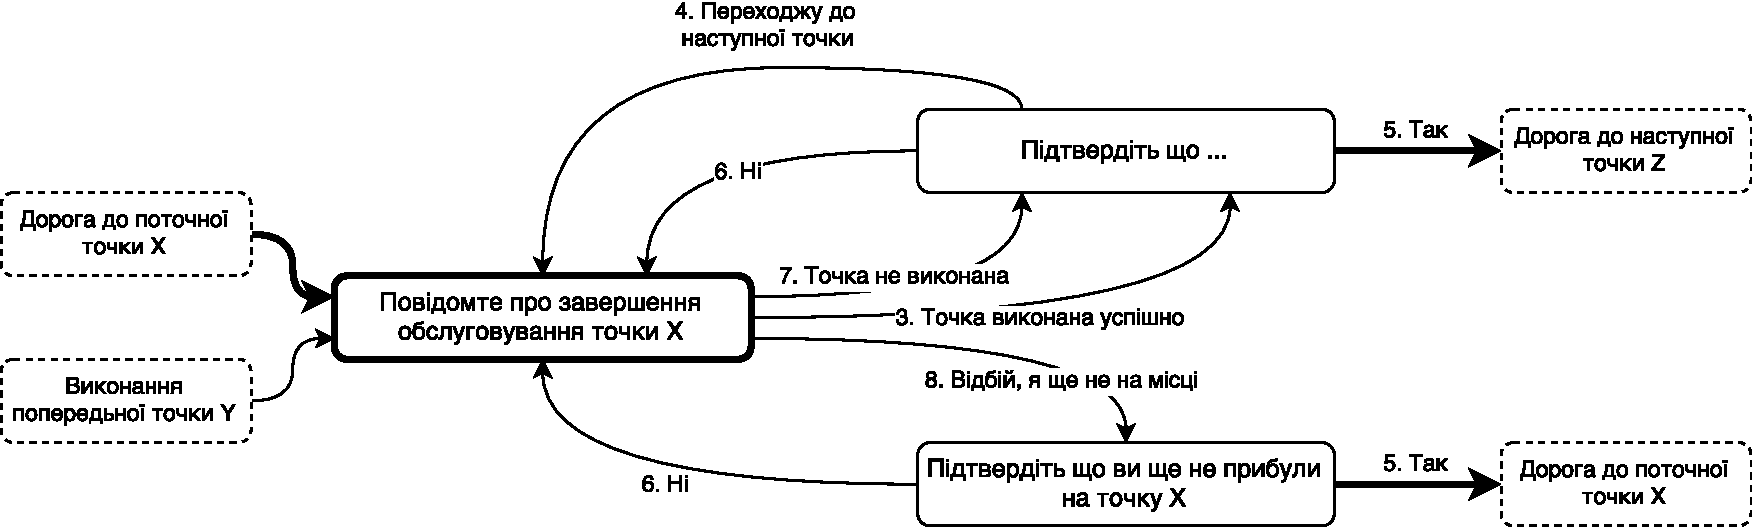
\includegraphics [width=1\linewidth] {07_simple_point_scenario_horizontal}
	\caption{Частина дерева сценаріїв етапу <<точка доставки>> в горизонтальному розподілі}
	\label{img:07_simple_point_scenario_horizontal}
\end{figure}
\begin{figure}
	\centering
	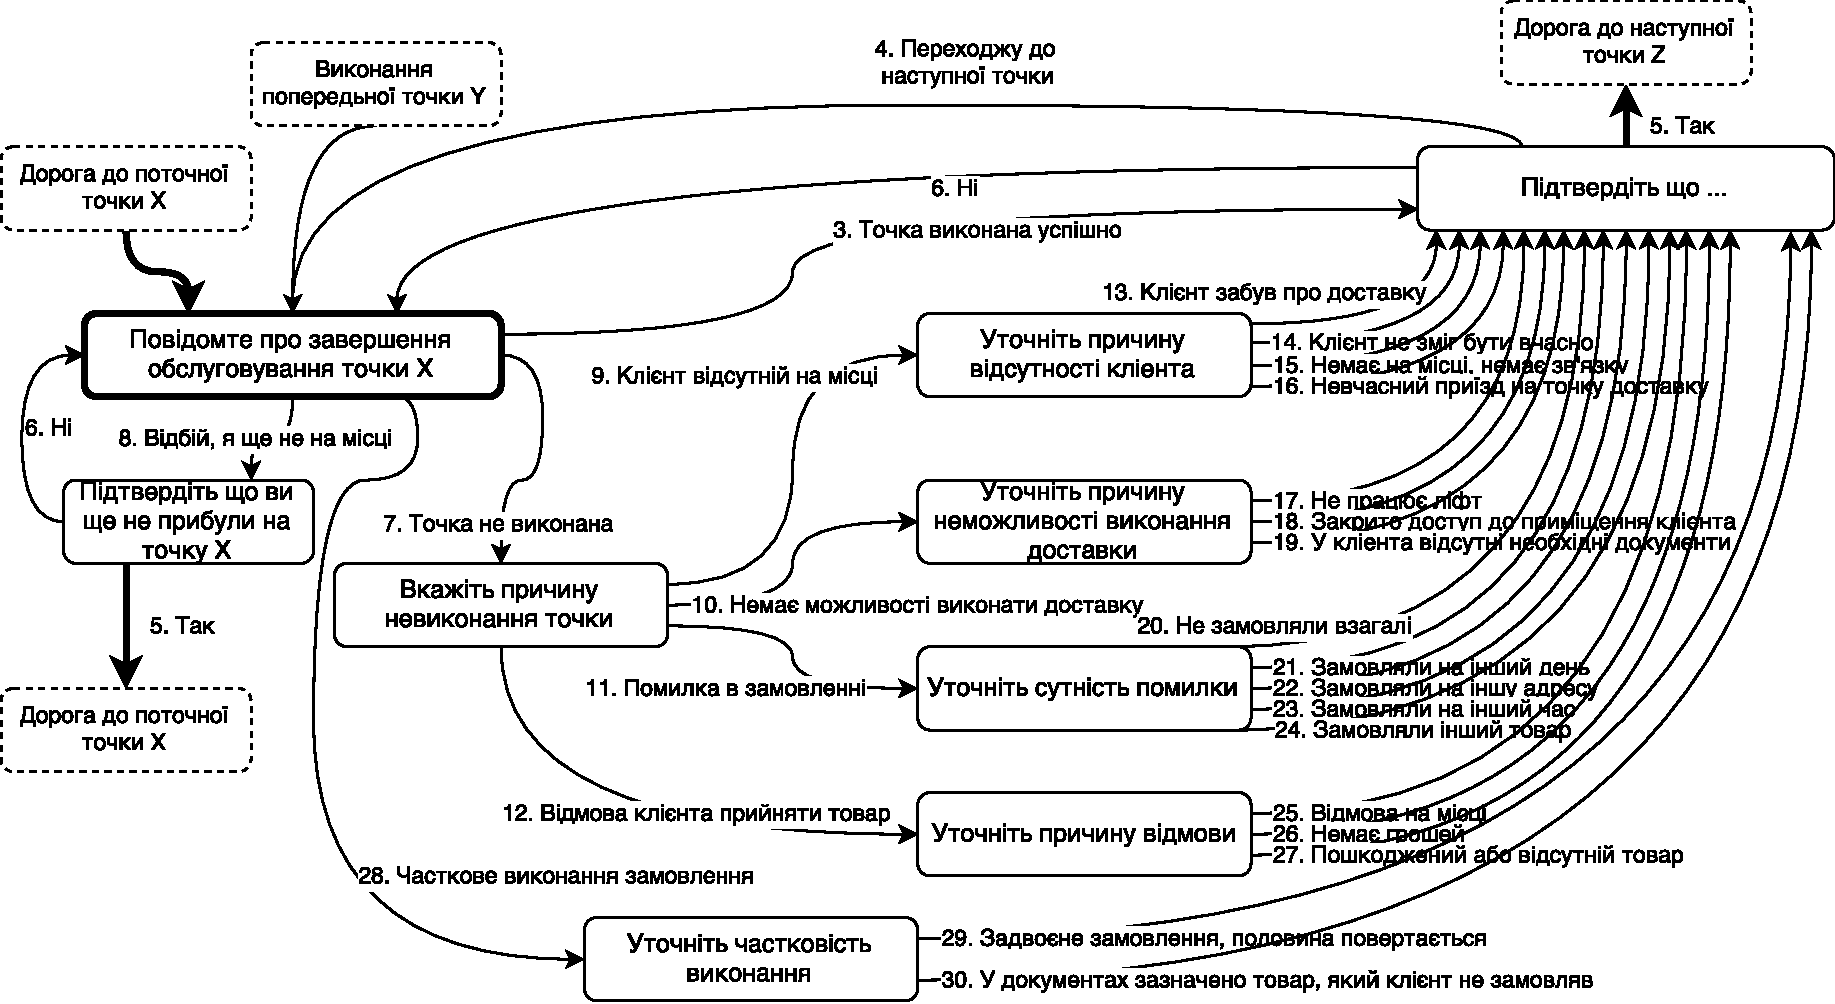
\includegraphics [width=1\linewidth] {08_complete_point_scenario}
	\caption{Частина дерева сценаріїв етапу <<точка доставки>> з усіма негативними інцидентами}
	\label{img:08_complete_point_scenario}
\end{figure}
\begin{figure}
	\centering
	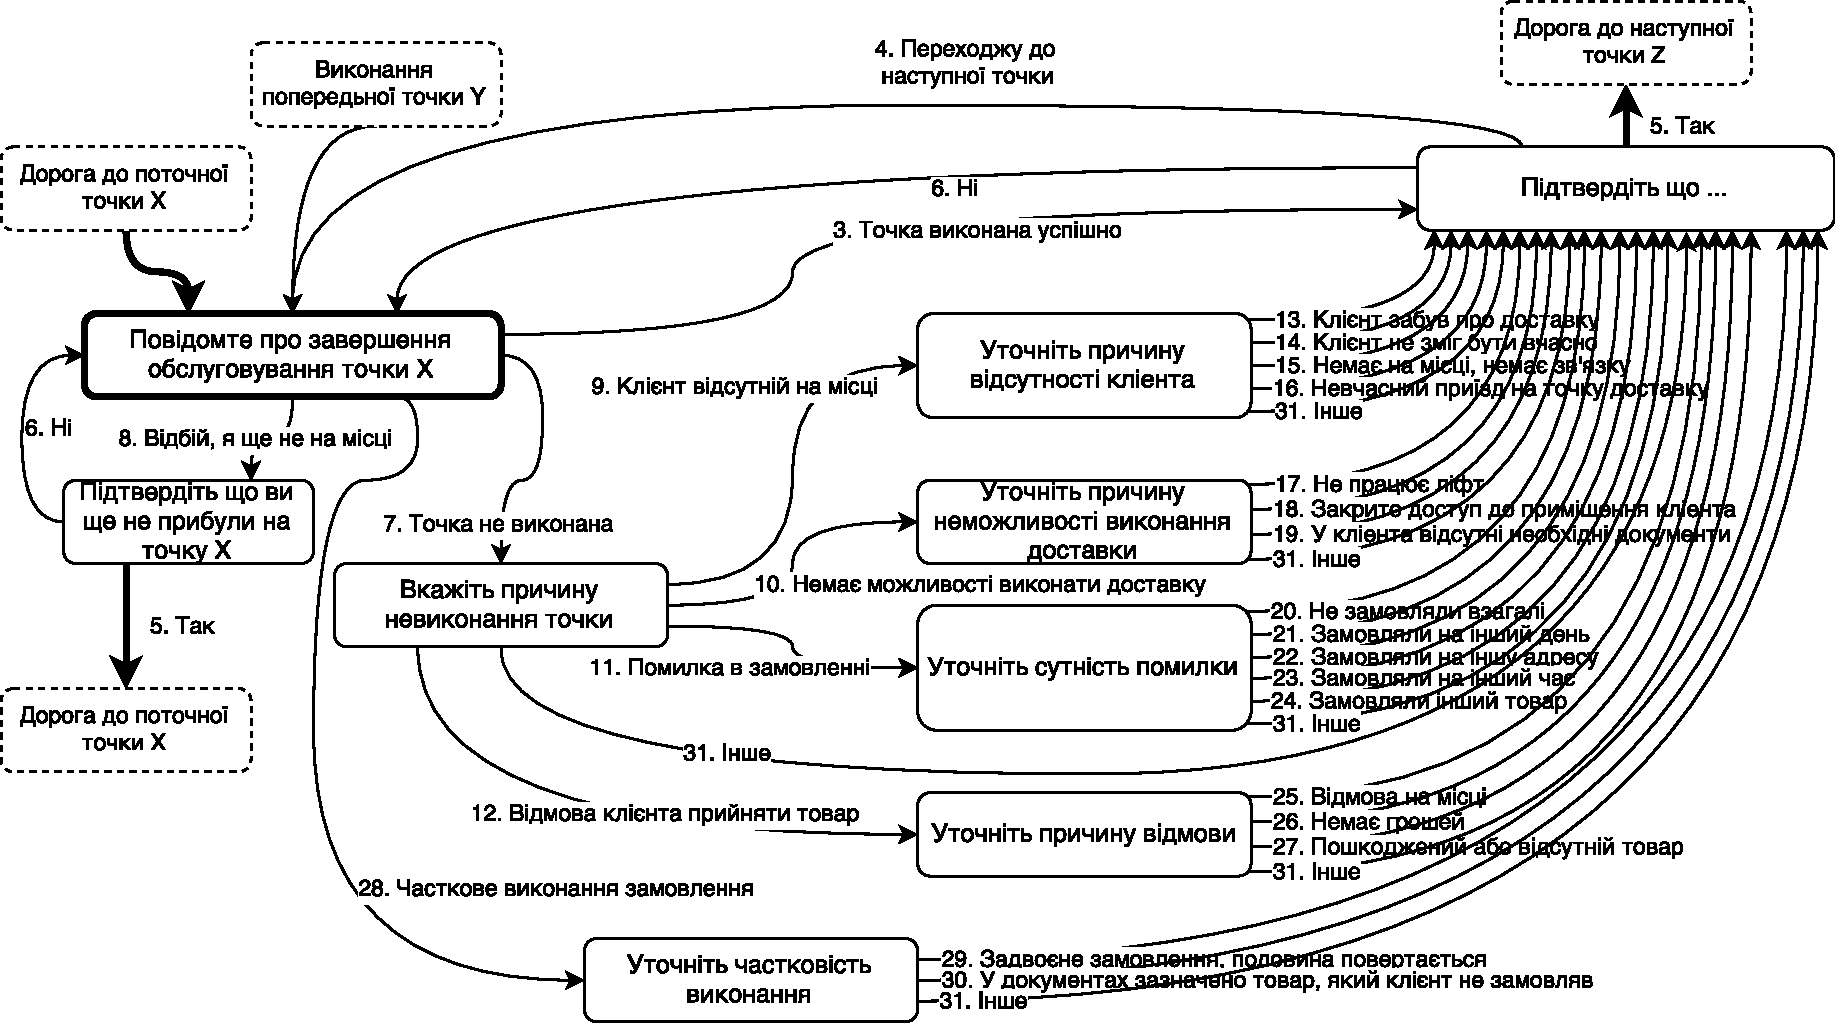
\includegraphics [width=1\linewidth] {08_complete_point_scenario_with_other}
	\caption{Частина дерева сценаріїв етапу <<точка доставки>> з усіма негативними інцидентами та урахуванням інших непередбачених подій}
	\label{img:08_complete_point_scenario_with_other}
\end{figure}
\begin{figure} 
	\centering
	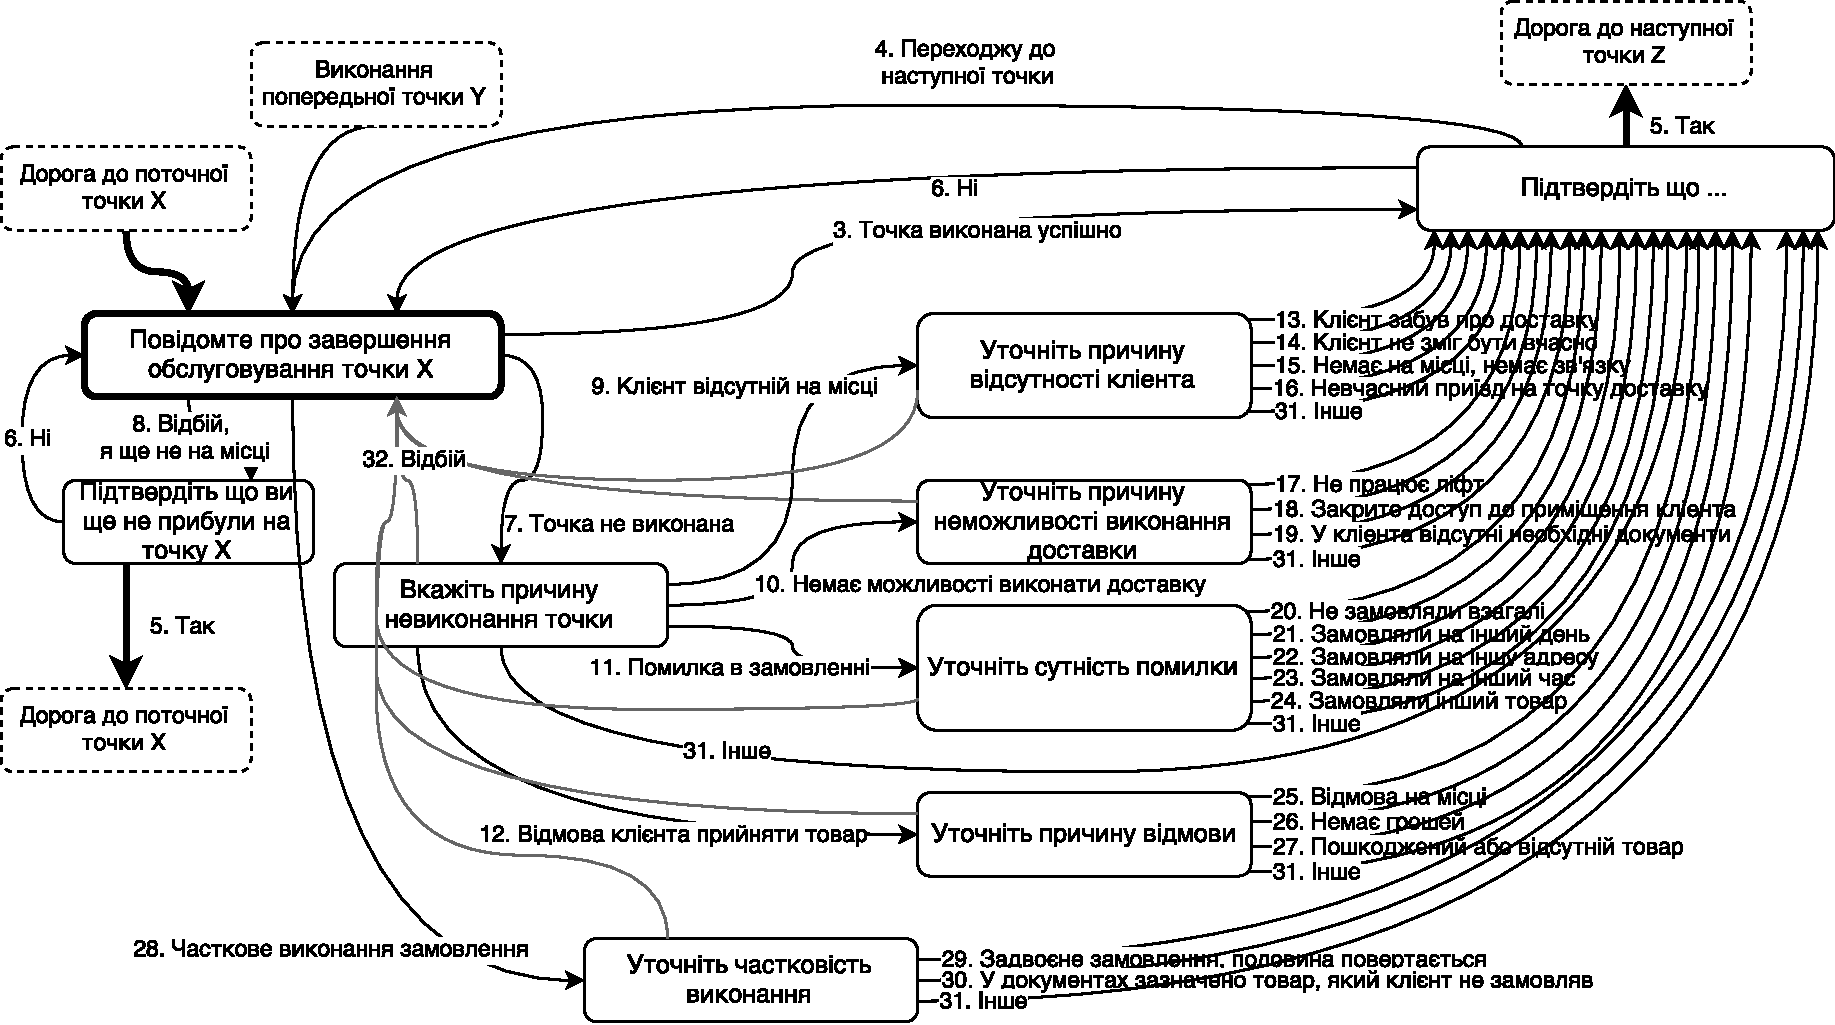
\includegraphics [width=1\linewidth] {09_complete_point_scenario_with_rollback}
	\caption{Частина дерева сценаріїв етапу "точка доставки" з усіма негативними інцидентами та відбоєм із діалогового режиму}
	\label{img:09_complete_point_scenario_with_rollback}
\end{figure}
\begin{figure}
	\centering
	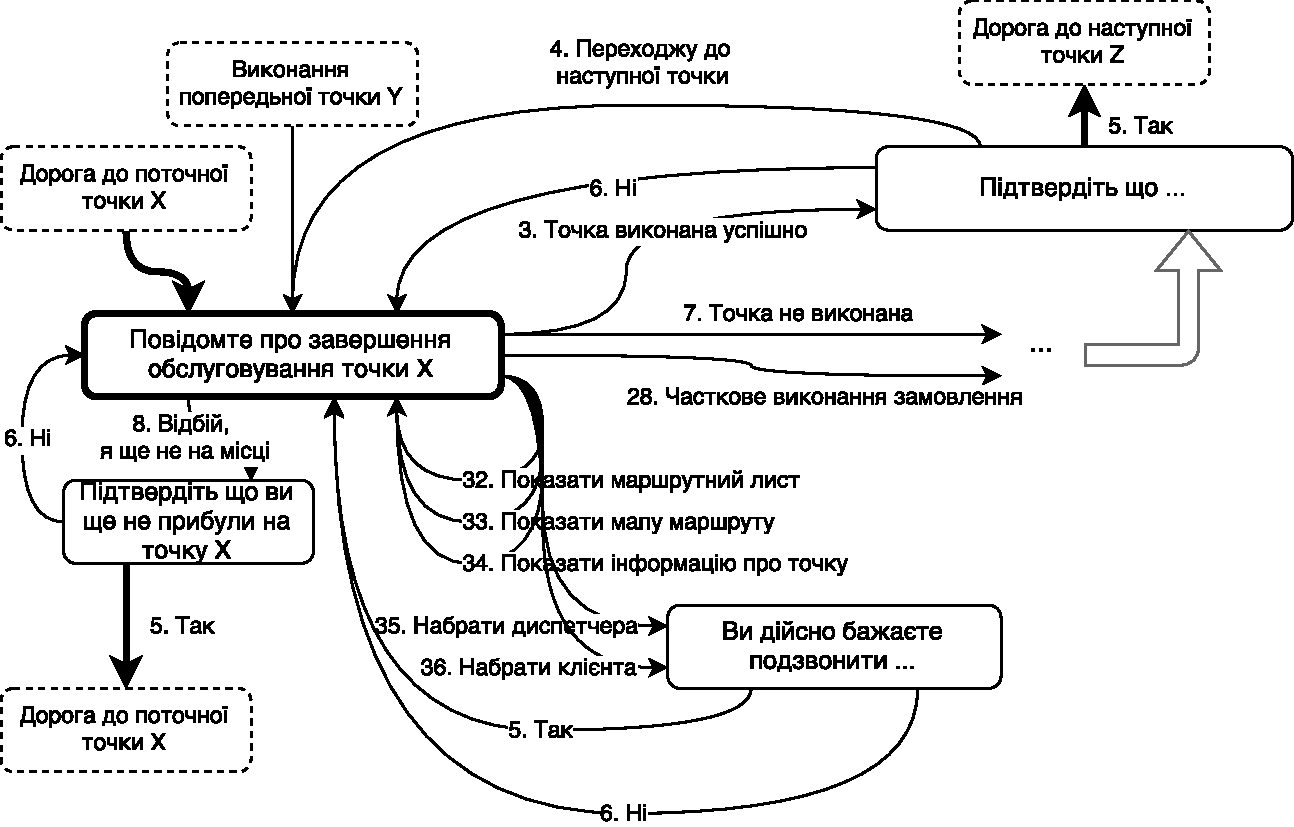
\includegraphics [width=1\linewidth] {10_point_scenario_with_enchantment}
	\caption{Частина дерева сценаріїв етапу <<точка доставки>> з додатковими функціями}
	\label{img:10_point_scenario_with_enchantment}
\end{figure}
\begin{figure}
	\centering
	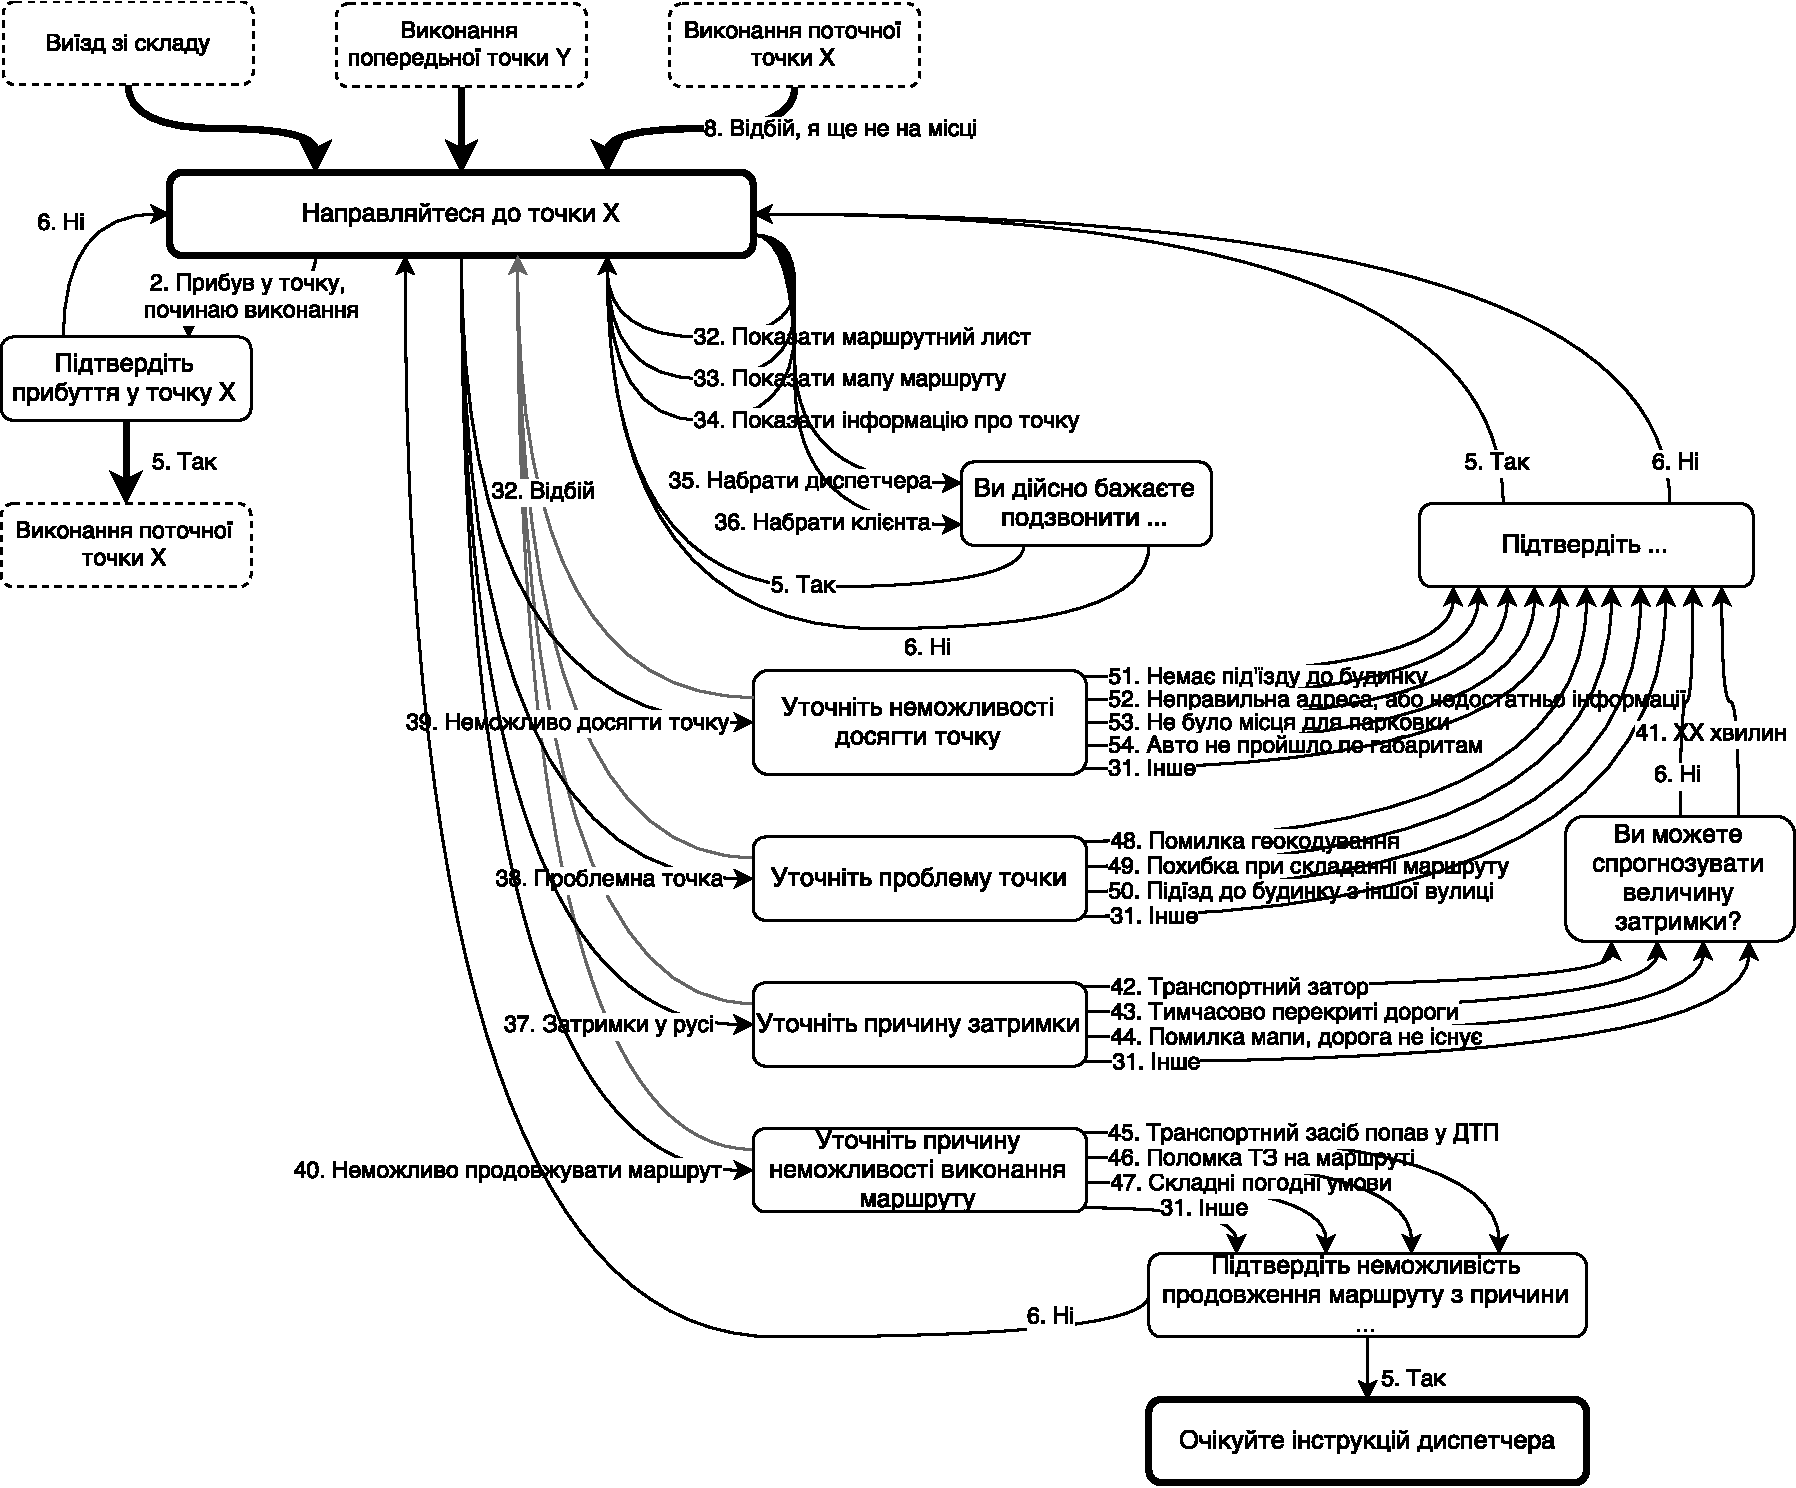
\includegraphics [width=.8\linewidth] {11_complete_road_scenario}
	\caption{Частина дерева сценаріїв етапу <<дорога>>}
	\label{img:11_complete_road_scenario}
\end{figure}
\begin{figure}
	\centering
	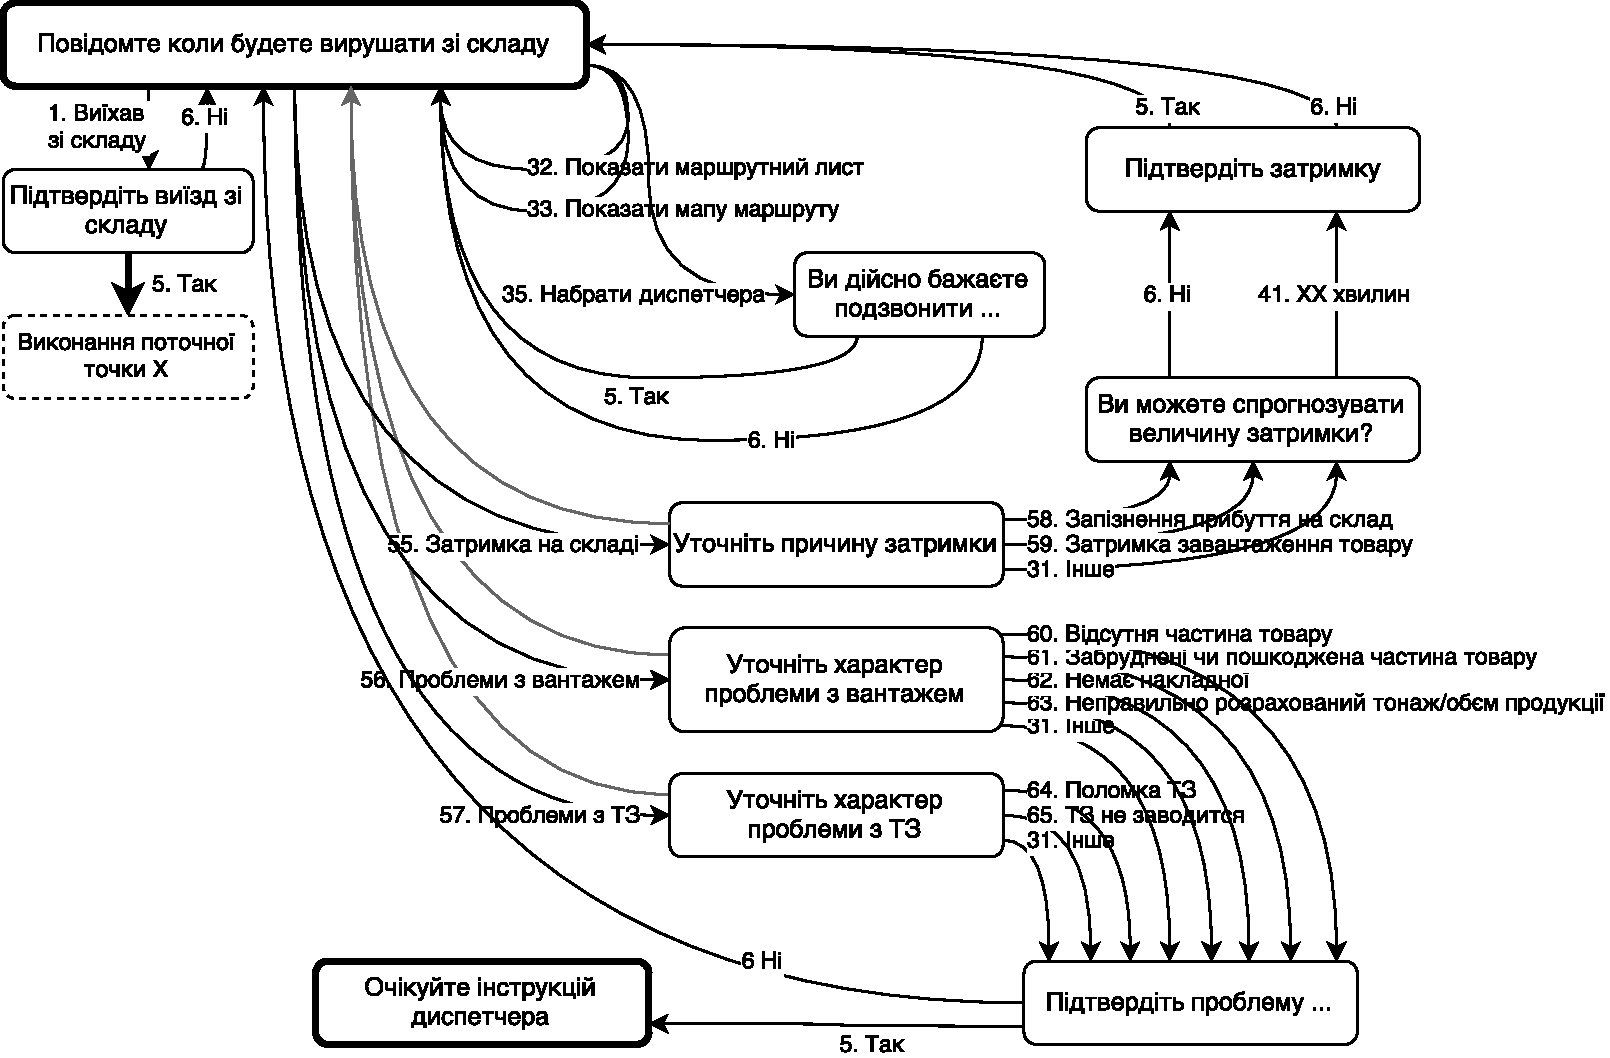
\includegraphics [width=.8\linewidth] {12_complete_depot_scenario}
	\caption{Частина дерева сценаріїв етапу <<склад>>}
	\label{img:12_complete_depot_scenario}
\end{figure}
\begin{figure}
	\centering
	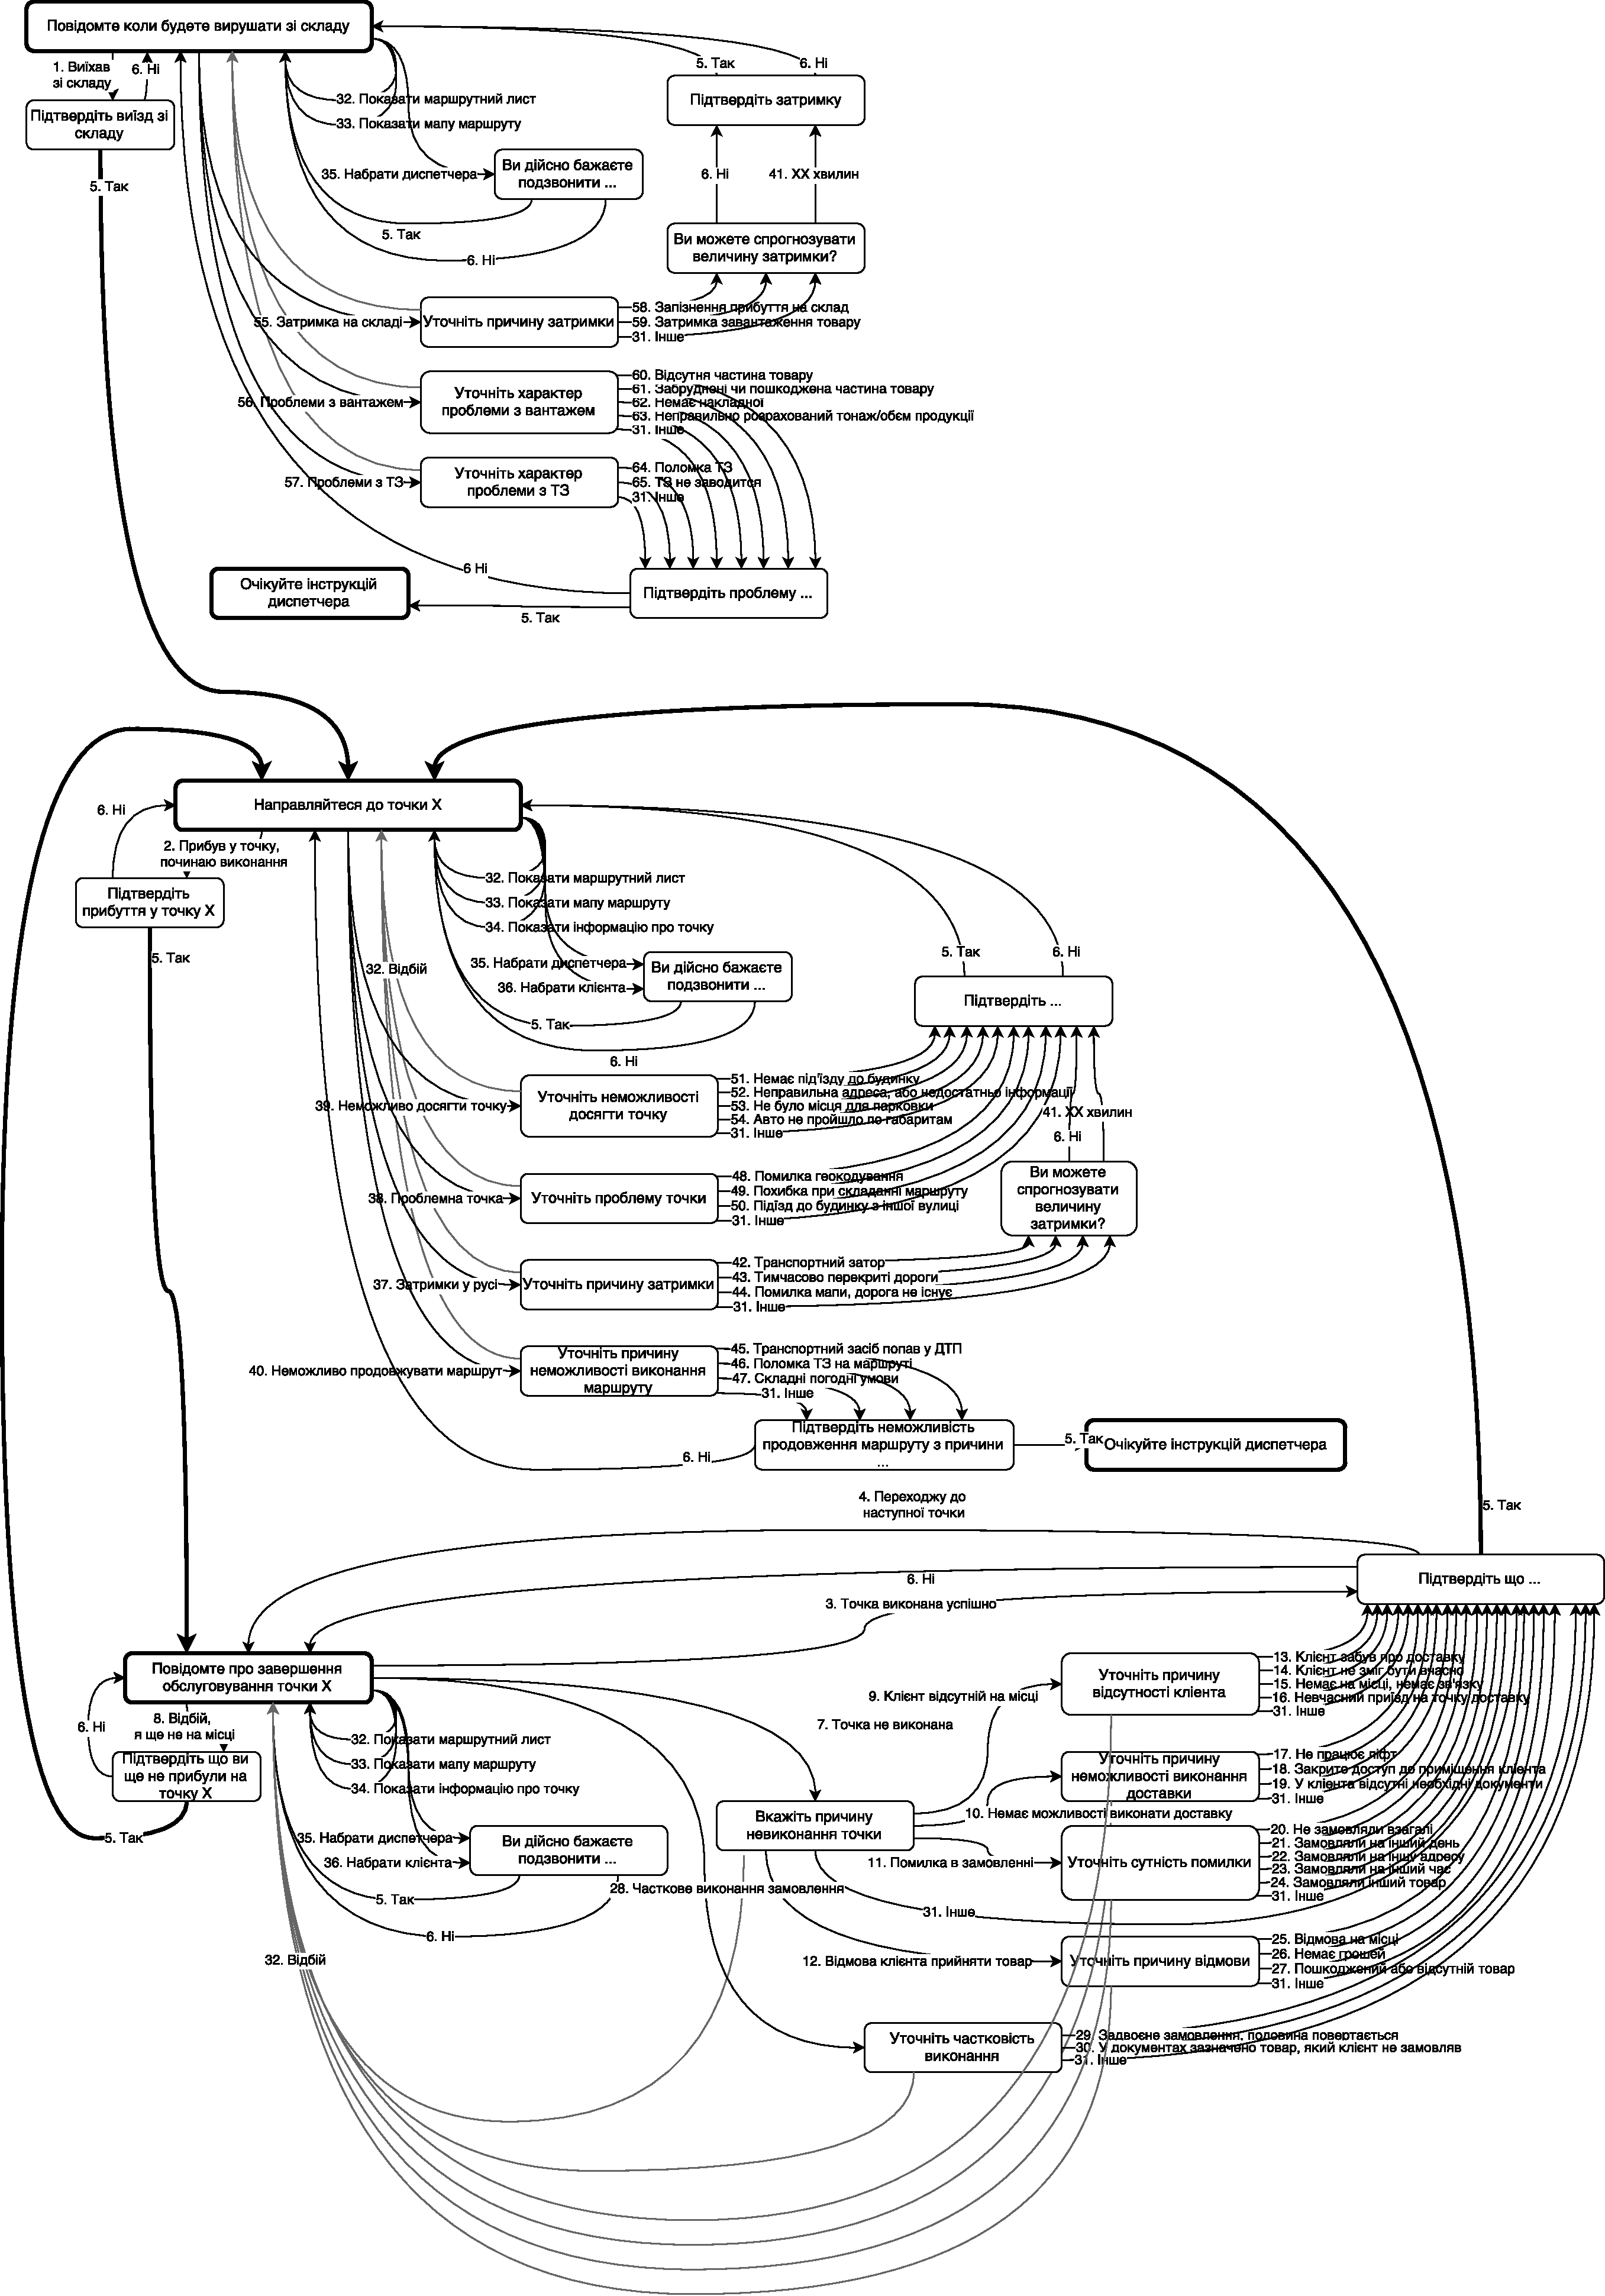
\includegraphics [width=1\linewidth] {13_complete_scenario_graph}
	\caption{Повне дерево сценаріїв всіх етапів}
	\label{img:13_complete_scenario_graph}
\end{figure}
\begin{mytable*}{ | c | l | }%
	{Різні варіанти стимулів з дерева сценаріїв}%
	{\label{tbl:scenario_commands}}%
	{№ & Варіанти стимулу}
	
	1 & Виїхав зі складу \\
	\hline
	2 & Прибув у точку, починаю виконання \\
	\hline
	3 & Точка виконана успішно \\
	\hline
	4 & Переходжу до наступної точки \\
	\hline
	5 & Так \\
	\hline
	6 & Ні \\
	\hline
	7 & Точка не виконана \\
	\hline
	8 & Відбій, я ще не на місці \\
	\hline
	9 & Клієнт відсутній на місці \\
	\hline
	10 & Немає можливості виконати доставку  \\
	\hline
	11 & Помилка в замовленні \\
	\hline
	12 & Відмова клієнта прийняти товар \\
	\hline
	13 & Клієнт забув про доставку \\
	\hline
	14 & Клієнт не зміг бути вчасно \\
	\hline
	15 & Немає на місці, немає звʼязку \\
	\hline
	16 & Невчасний приїзд на точку доставку \\
	\hline
	17 & Не працює ліфт \\
	\hline
	18 & Закрито доступ до приміщення клієнта \\
	\hline
	19 & У клиента відсутні необхідні документи \\
	\hline
	20 & Не замовляли взагалі \\
	\hline
	21 & Замовляли на інший день \\
	\hline
	22 & Замовляли на іншу адресу \\
	\hline
	23 & Замовляли на інший час \\
	\hline
	24 & Замовляли інший товар \\
	\hline
	25 & Відмова на місці \\
	\hline
	26 & Немає грошей \\
	\hline
	27 & Пошкоджений або відсутній товар \\
	\hline
	28 & Часткове виконання замовлення \\
	\hline
	29 & Задвоєне замовлення, половина повертається \\
	\hline
	30 & У документах зазначено товар, який клієнт не замовляв \\
	\hline
	31 & Інше \\
	\hline
	32 & Показати маршрутний лист \\
	\hline
	33 & Показати мапу маршруту \\
	\hline
	34 & Показати інформацію про точку \\
	\hline
	35 & Набрати диспетчера \\
	\hline
	36 & Набрати клієнта \\
	\hline
	37 & Затримки у русі \\
	\hline
	38 & Проблемна точка \\
	\hline
	39 & Неможливо досягти точку \\
	\hline
	40 & Неможливо продовжувати маршрут \\
	\hline
	41 & \# хвилин \\
	\hline
	42 & Транспортний затор \\
	\hline
	43 & Тимчасово перекриті дороги \\
	\hline
	44 & Помилка мапи, дорога не існує \\
	\hline
	45 & Транспортний засіб попав у ДТП \\
	\hline
	46 & Поломка ТЗ на маршруті \\
	\hline
	47 & Складні погодні умови \\
	\hline
	48 & Помилка геокодування \\
	\hline
	49 & Похибка при складанні маршруту \\
	\hline
	50 & Підʼїзд до будинку з іншої вулиці \\
	\hline
	51 & Немає підʼїзду до будинку \\
	\hline
	52 & Неправильна адреса, або недостатньо інформації \\
	\hline
	53 & Не було місця для парковки \\
	\hline
	54 & Авто не пройшло по габаритам \\
	\hline
	55 & Затримка на складі \\
	\hline
	56 & Проблеми з вантажем \\
	\hline
	57 & Проблеми з ТЗ \\
	\hline
	58 & Запізнення прибуття на склад \\
	\hline
	59 & Затримка завантаження товару \\
	\hline
	60 & Відсутня частина товару \\
	\hline
	61 & Забруднені чи пошкоджена частина товару \\
	\hline
	62 & Немає накладної \\
	\hline
	63 & Неправильно розрахований тоннаж/обʼєм продукції \\
	\hline
	64 & Поломка ТЗ \\
	\hline
	65 & ТЗ не заводится \\
\end{mytable*}%
\begin{figure}
	\centering
	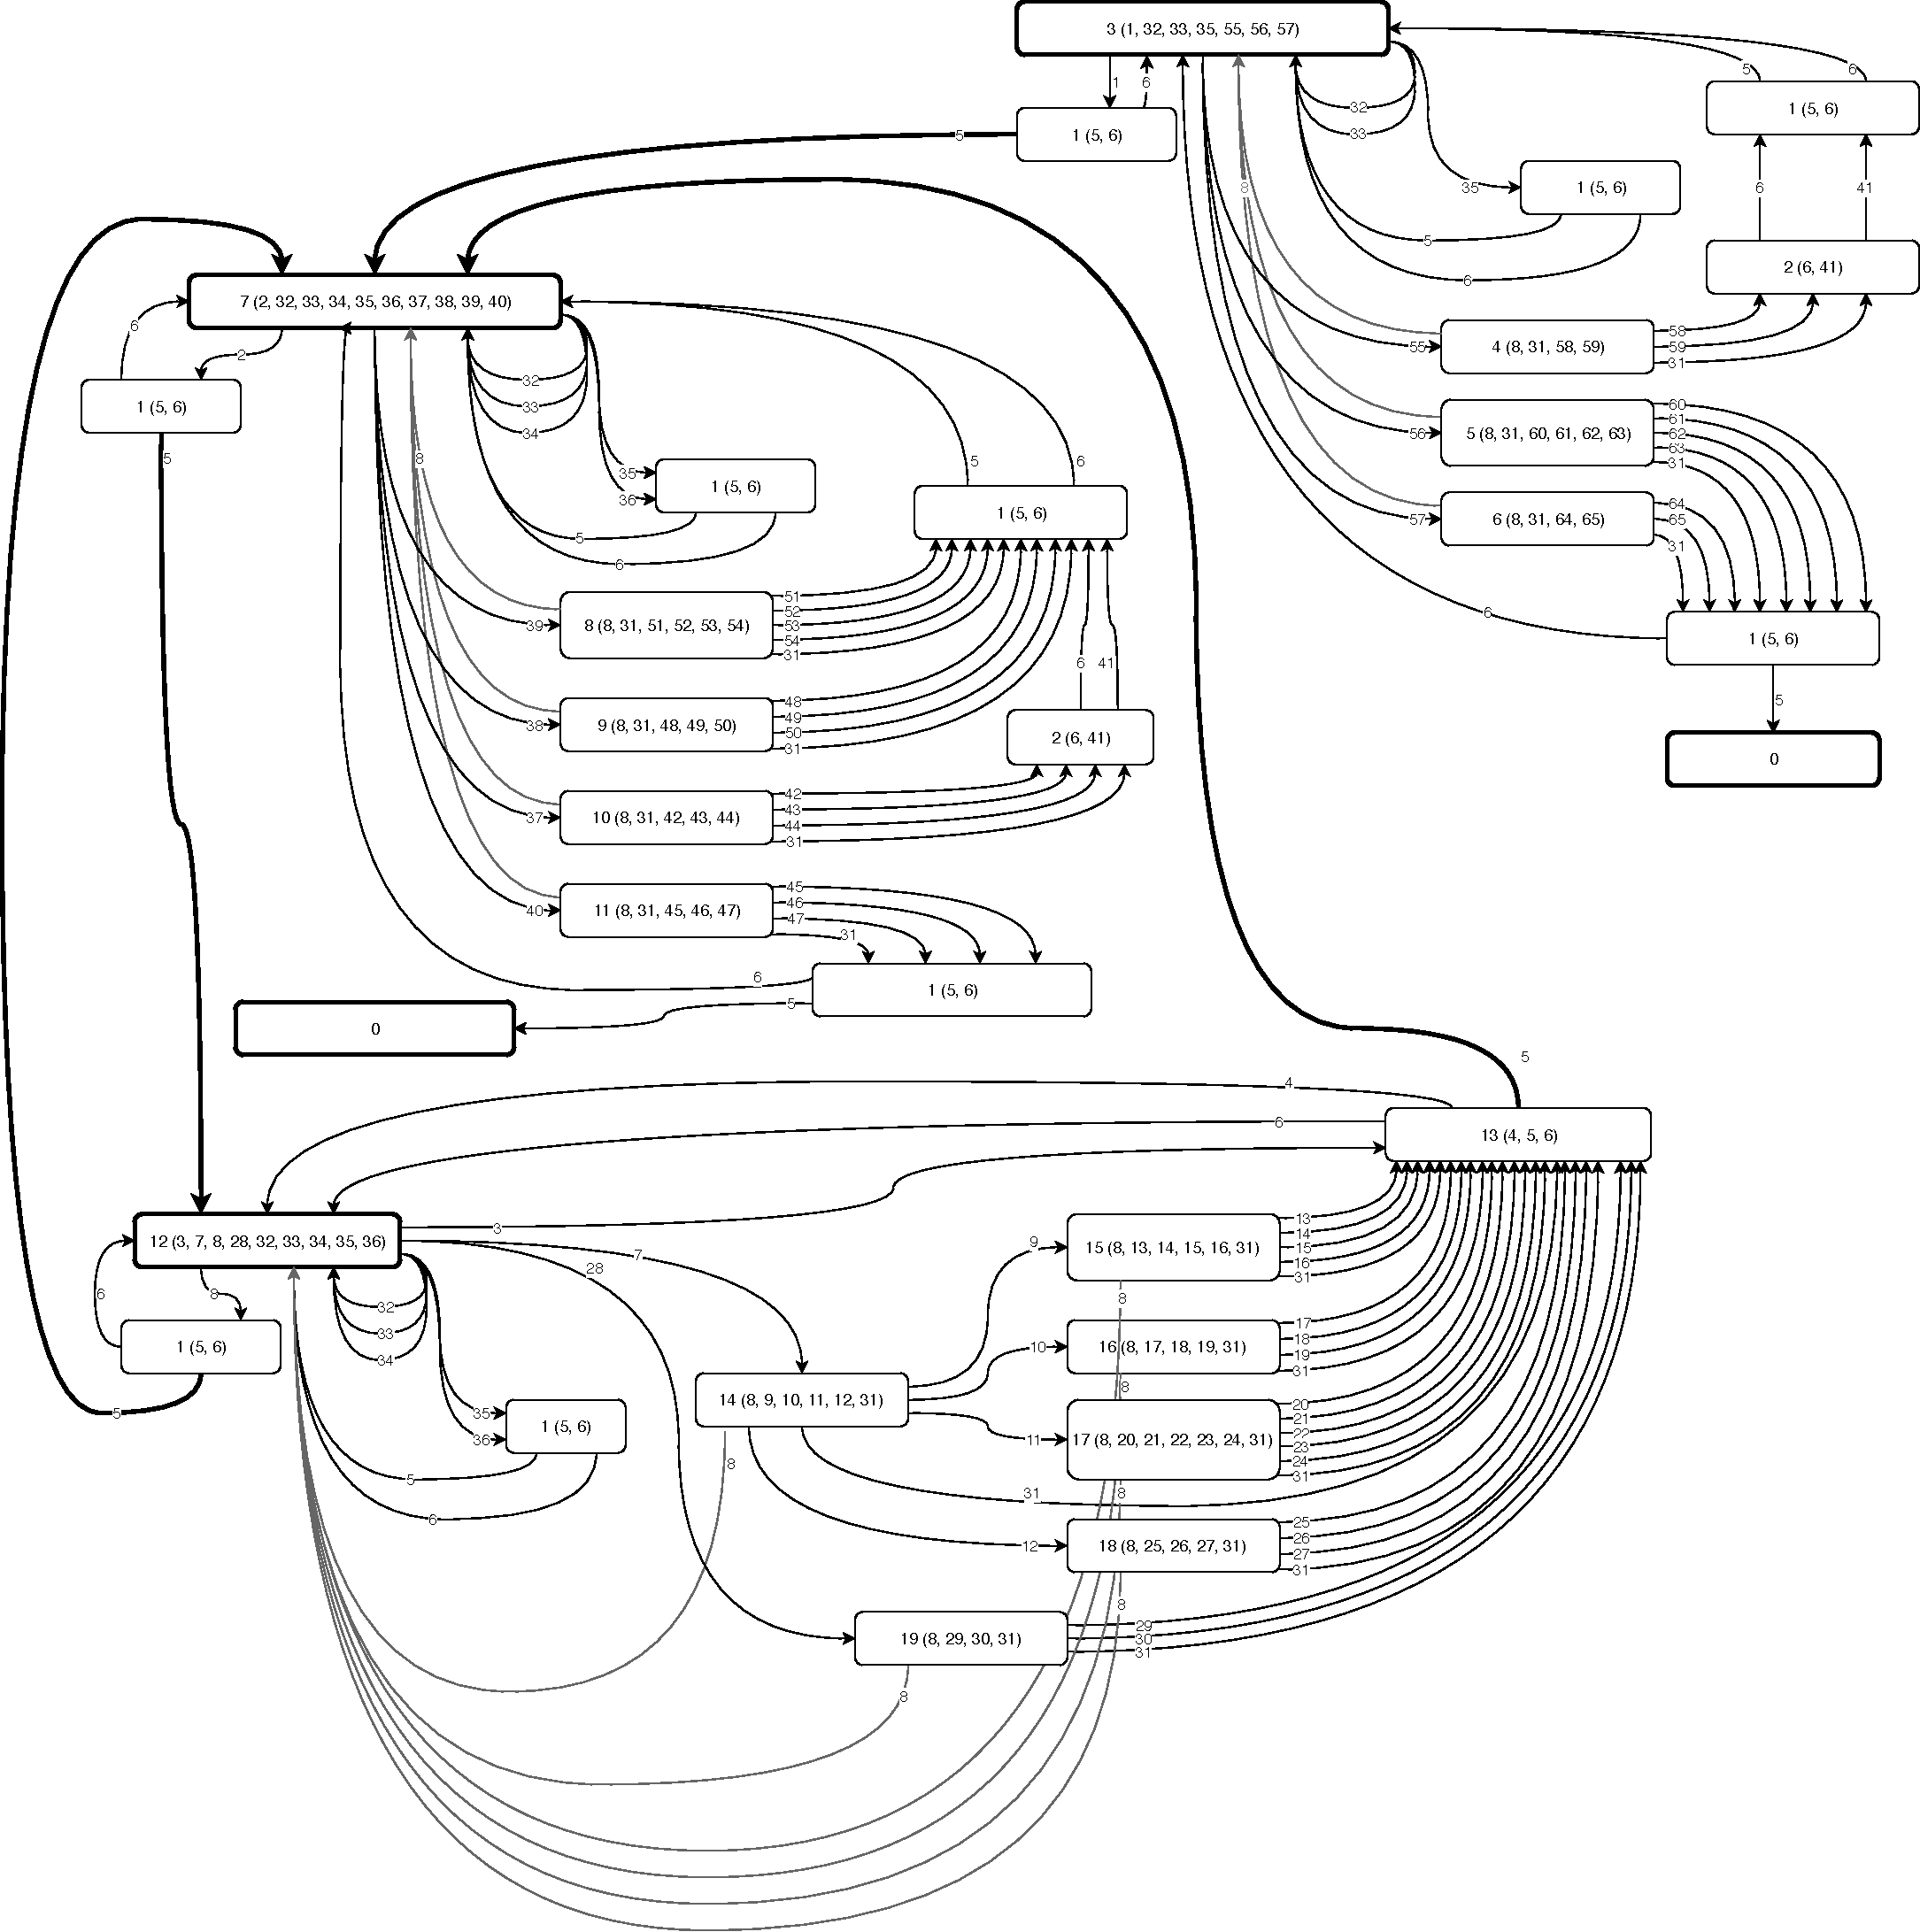
\includegraphics [width=1\linewidth] {14_complete_scenario_graph_contexts}
	\caption{Повне дерево сценаріїв всіх етапів з указанням контекстів}
	\label{img:14_complete_scenario_graph_contexts}
\end{figure}
\begin{mytable}{ | c | l | }%
	{Перелік контекстів та можливих реакцій у них}%
	{\label{tbl:context_reactions}}%
	{№ & Можливі реакції}
	
	1 & 5, 6 \\
	\hline
	2 & 6, 41 \\
	\hline
	3 & 1, 32, 33, 35, 55, 56, 57 \\
	\hline
	4 & 8, 31, 58, 59 \\
	\hline
	5 & 8, 31, 60, 61, 62, 63 \\
	\hline
	6 & 8, 31, 64, 65 \\
	\hline
	7 & 2, 32, 33, 34, 35, 36, 37, 38, 39, 40 \\
	\hline
	8 & 8, 31, 51, 52, 53, 54 \\
	\hline
	9 & 8, 31, 48, 49, 50 \\
	\hline
	10 & 8, 31, 42, 43, 44  \\
	\hline
	11 & 8, 31, 45, 46, 47 \\
	\hline
	12 & 3, 7, 8, 28, 32, 33, 34, 35, 36 \\
	\hline
	13 & 4, 5, 6 \\
	\hline
	14 & 8, 9, 10, 11, 12, 31 \\
	\hline
	15 & 8, 13, 14, 15, 16, 31 \\
	\hline
	16 & 8, 17, 18, 19, 31 \\
	\hline
	17 & 8, 20, 21, 22, 23, 24, 31 \\
	\hline
	18 & 8, 25, 26, 27, 31 \\
	\hline
	19 & 8, 29, 30, 31 \\
\end{mytable}%
\begin{figure}
	\centering
	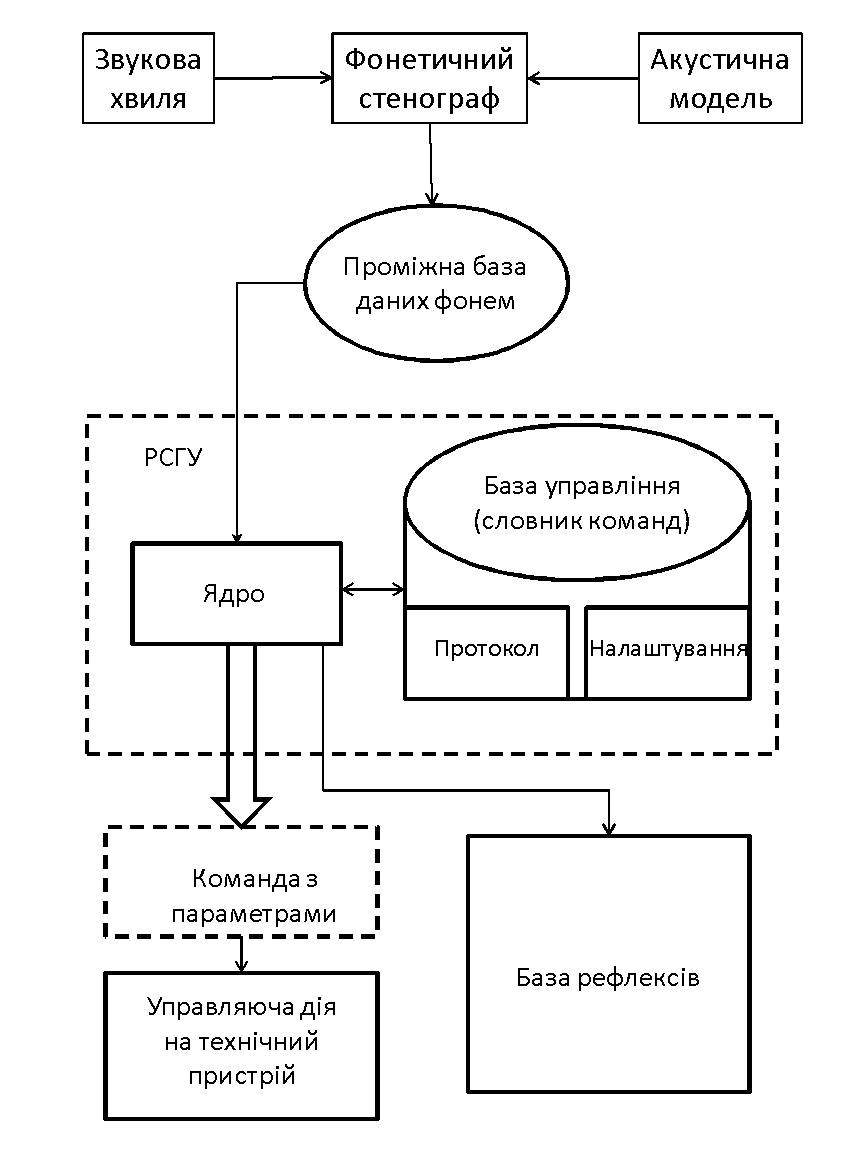
\includegraphics [width=.5\linewidth] {rsgu_struct}
	\caption{Структура системи формалізації голосової інформації в моделі голосової взаємодії водія при диспетчерському контролі за рухом автотранспорту}
	\label{img:rsgu_struct}
\end{figure}
\begin{figure}
	\centering
	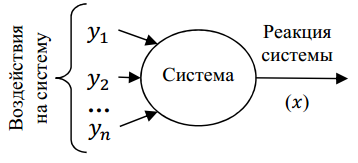
\includegraphics [width=.5\linewidth] {rsgu_scheme}
	\caption{Схема реакції системи формалізації голосової інформації в моделі голосової взаємодії водія при диспетчерському контролі за рухом автотранспорту на несилові впливи}
	\label{img:rsgu_scheme}
\end{figure}
\begin{figure}
	\centering
	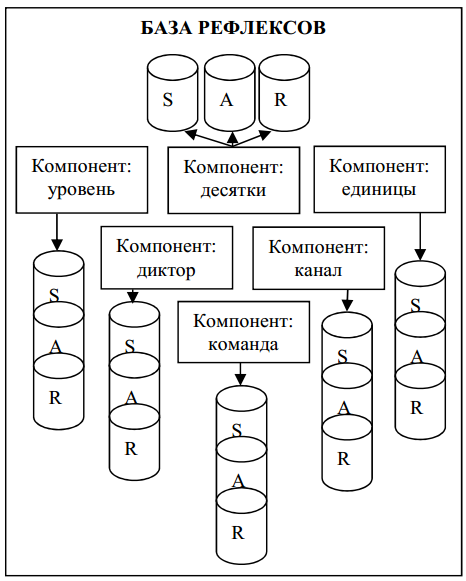
\includegraphics [width=.5\linewidth] {rsgu_base}
	\caption{Структура бази рефлексів системи формалізації голосової інформації}
	\label{img:rsgu_base}
\end{figure}
\begin{figure}[h!]
	\centering
	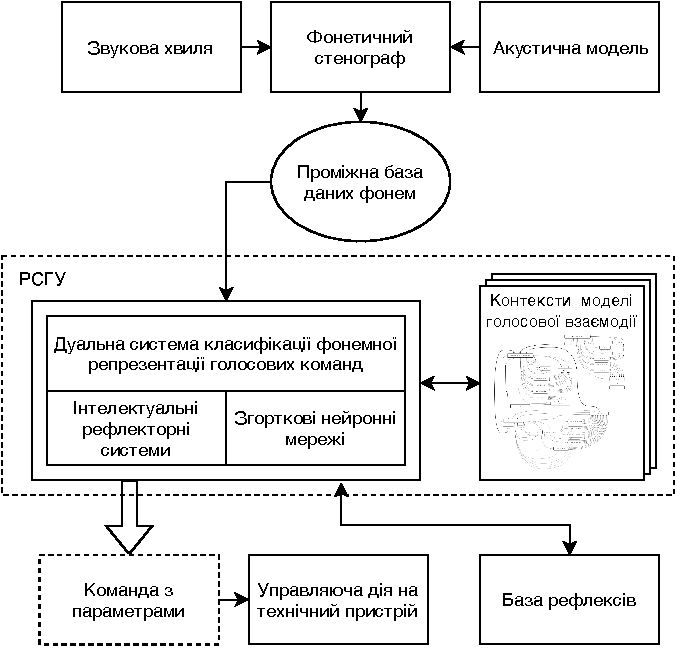
\includegraphics [width=.6\linewidth] {rsgu_struct_new}
	\caption{Удосконалена схема системи формалізації голосової інформації в моделі голосової взаємодії водія при диспетчерському контролі за рухом автотранспорту}
	\label{img:rsgu_struct_new}
\end{figure}
\begin{figure}
	\centering
	\subbottom[\label{img:cnn-struct1}]{%
		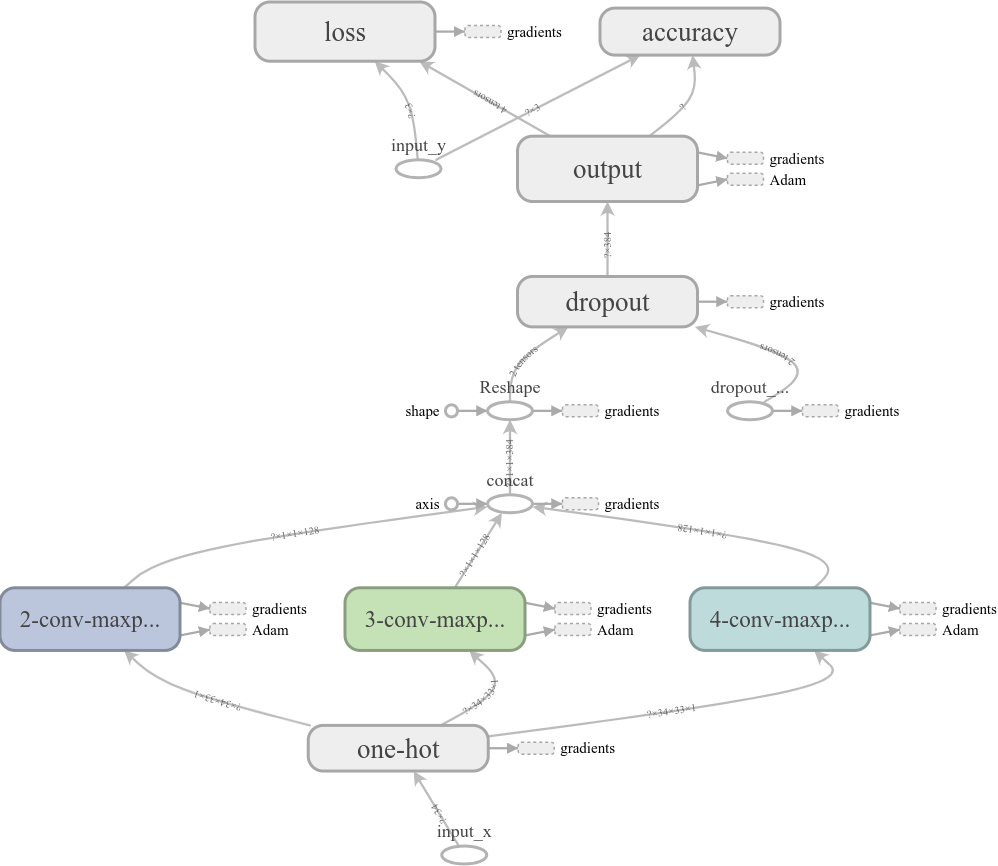
\includegraphics[width=.7\linewidth]{cnn_1}}
	\hfill
	\subbottom[\label{img:cnn-struct2}]{%
		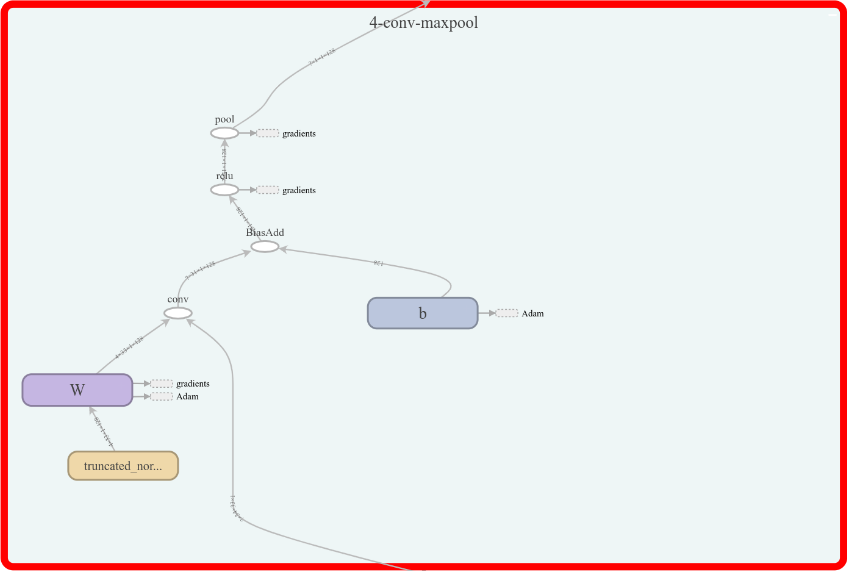
\includegraphics[width=.25\linewidth]{cnn_2}}
	\caption{Структура згорткової нейронної мережі (\subcaptionref{img:cnn-struct1}) та деталізація її згорткового шару (\subcaptionref{img:cnn-struct2})}
	\label{img:cnn-struct}
\end{figure}
\begin{figure}
	\centering
	\hspace{0pt plus1fill}
	\subbottom[\label{img:app-no1}]{%
		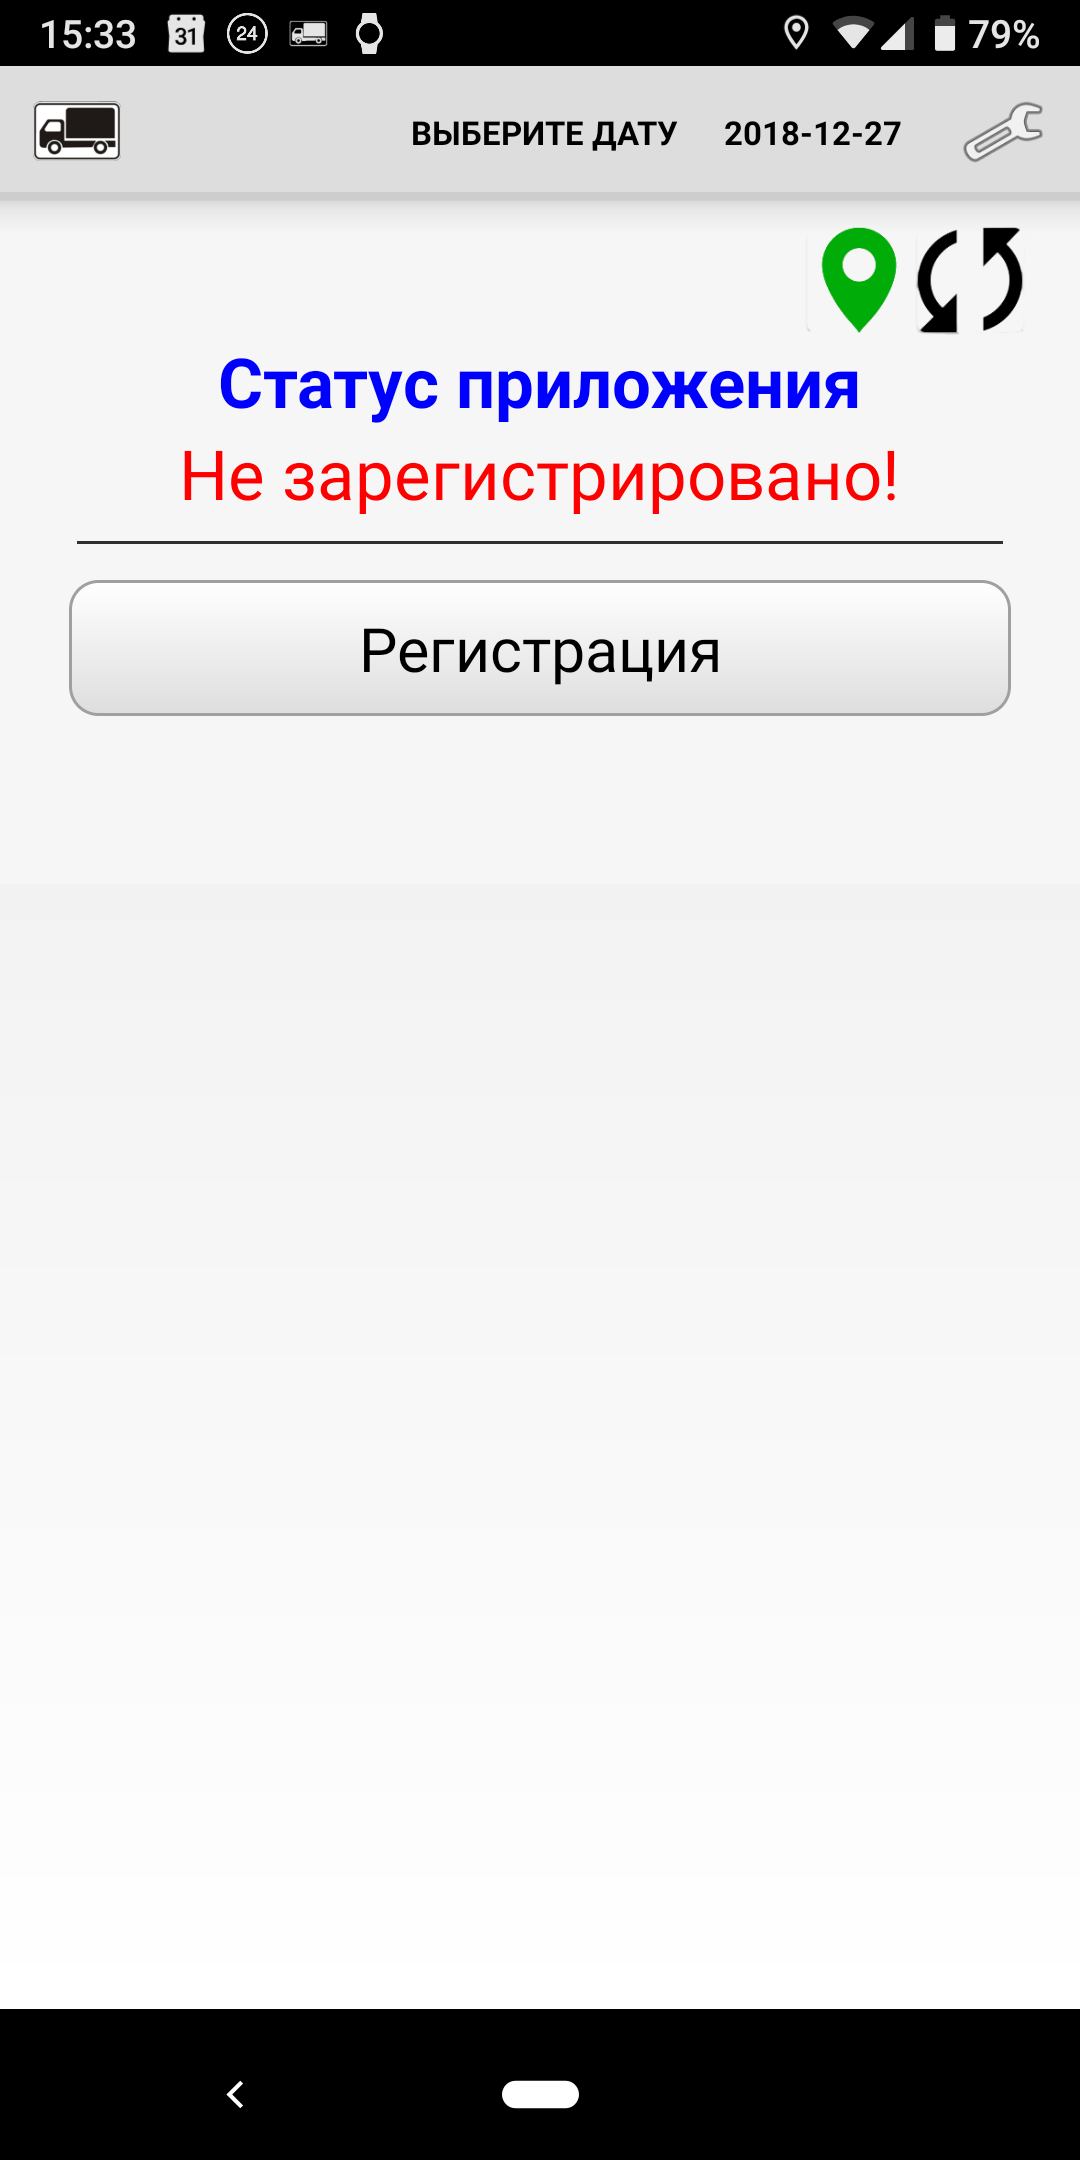
\includegraphics[width=.32\linewidth]{app-no1}}
	\hspace{0pt plus2fill}
	\subbottom[\label{img:app-no2}]{%
		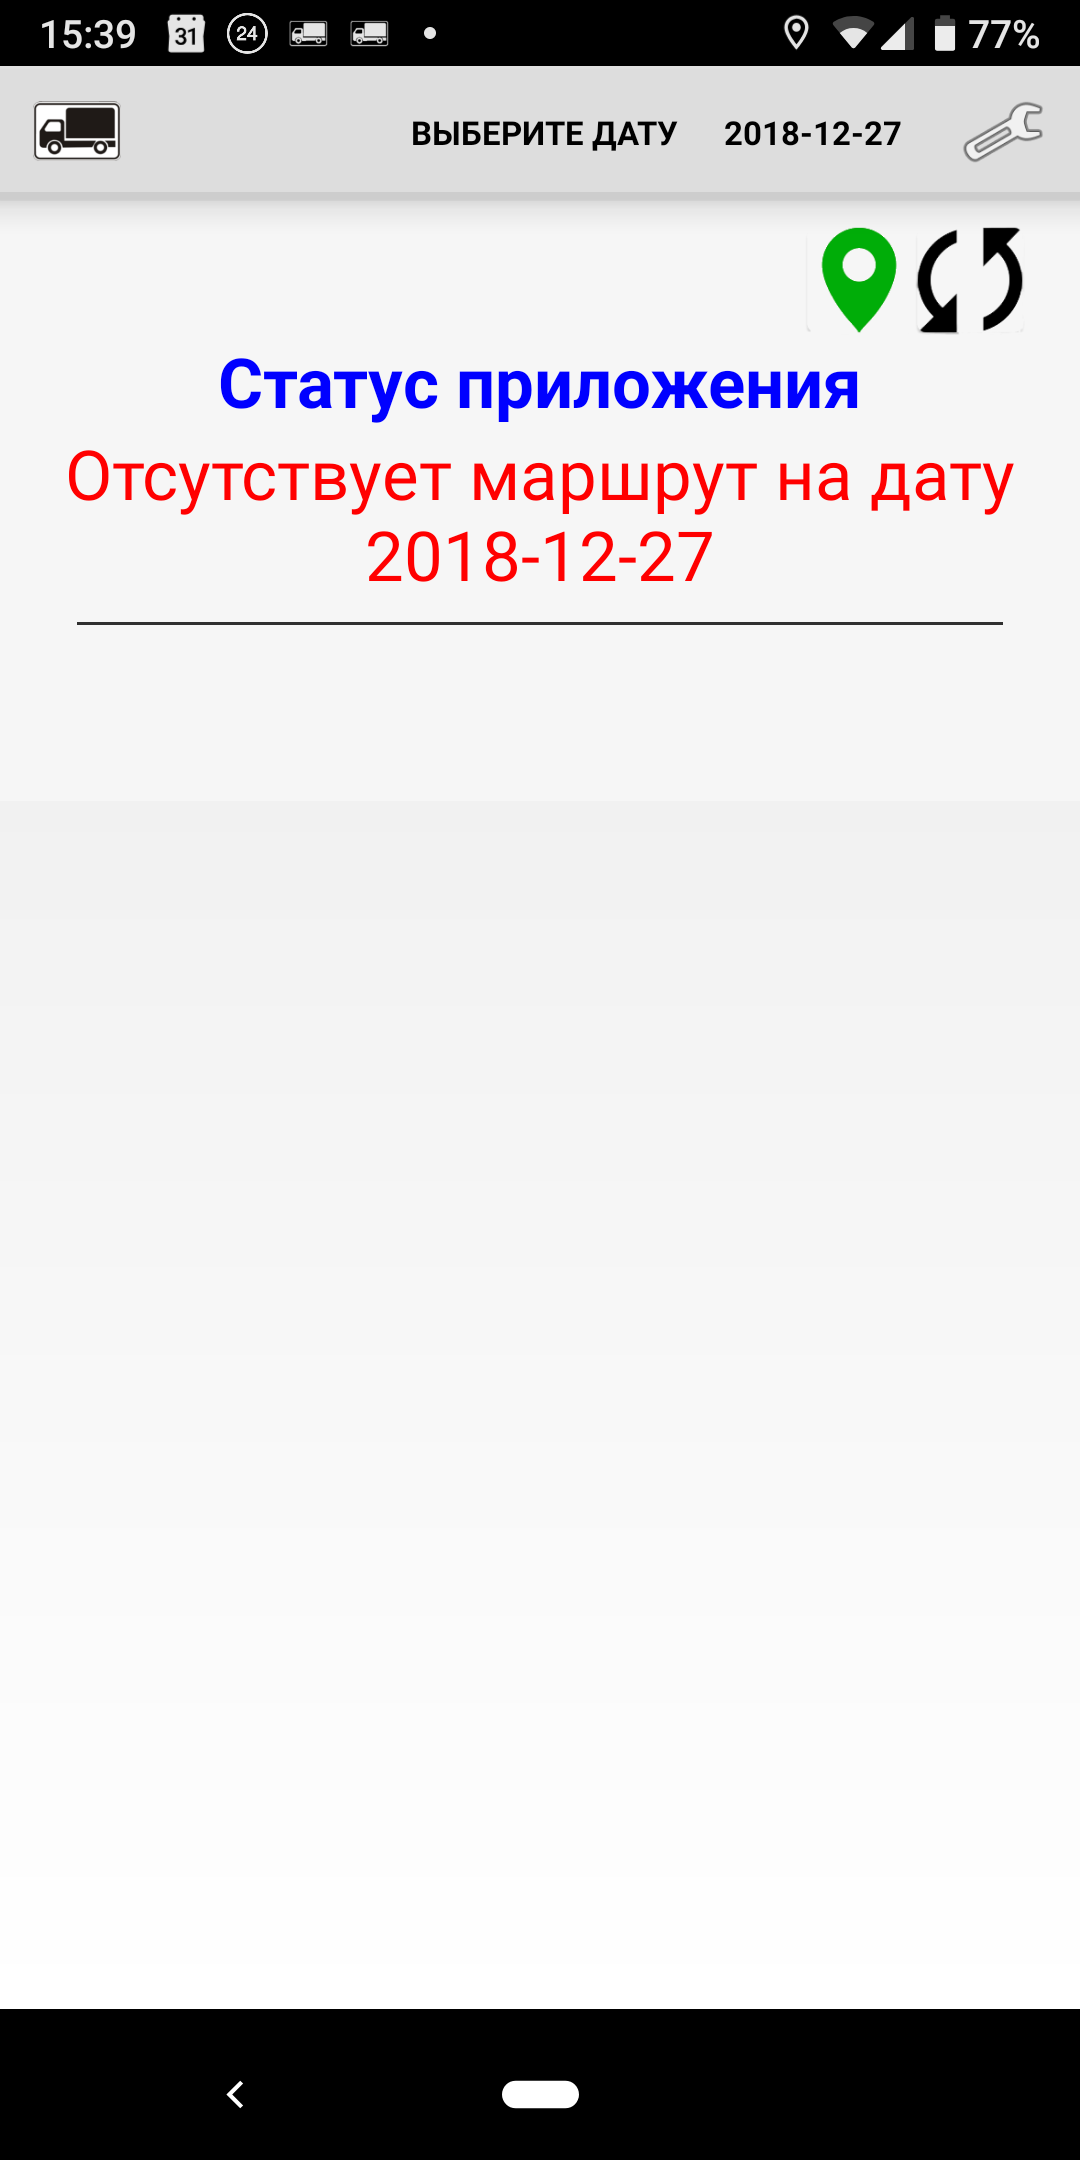
\includegraphics[width=.32\linewidth]{app-no2}}
	\hspace{0pt plus2fill}
	\subbottom[\label{img:app-opt}]{%
		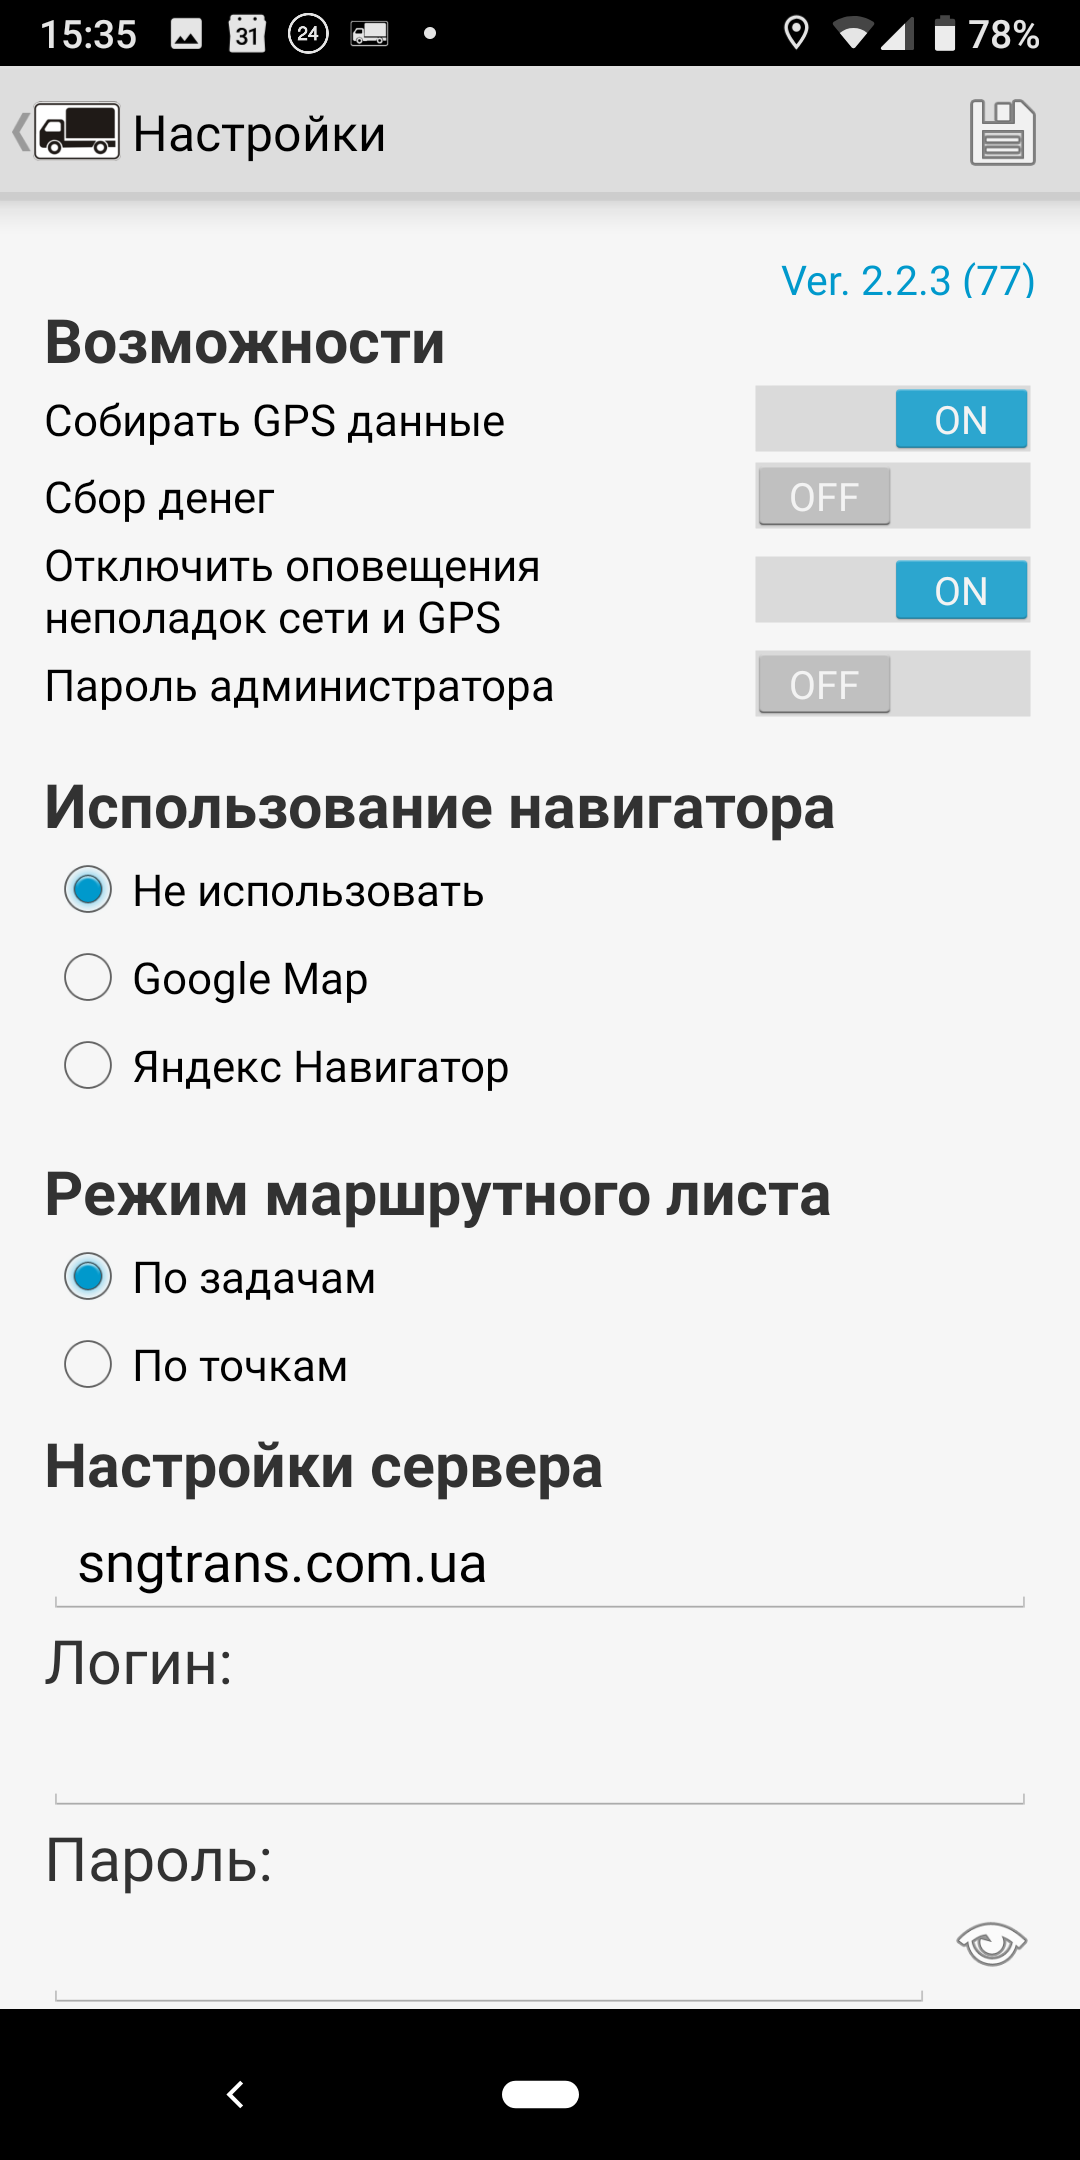
\includegraphics[width=.32\linewidth]{app-opt}}
	\hspace{0pt plus1fill}
	\caption{Вигляд інтерфейсу додатка для незареєстрованого пристрою (\subcaptionref{img:app-no1}), для випадку коли маршрут на вибрану дату відсутній (\subcaptionref{img:app-no2}) та вікно налаштувань (\subcaptionref{img:app-opt})}
	\label{img:app-base}
\end{figure}
\begin{figure}
	\centering
	\hspace{0pt plus1fill}
	\subbottom[\label{img:app-info1}]{%
		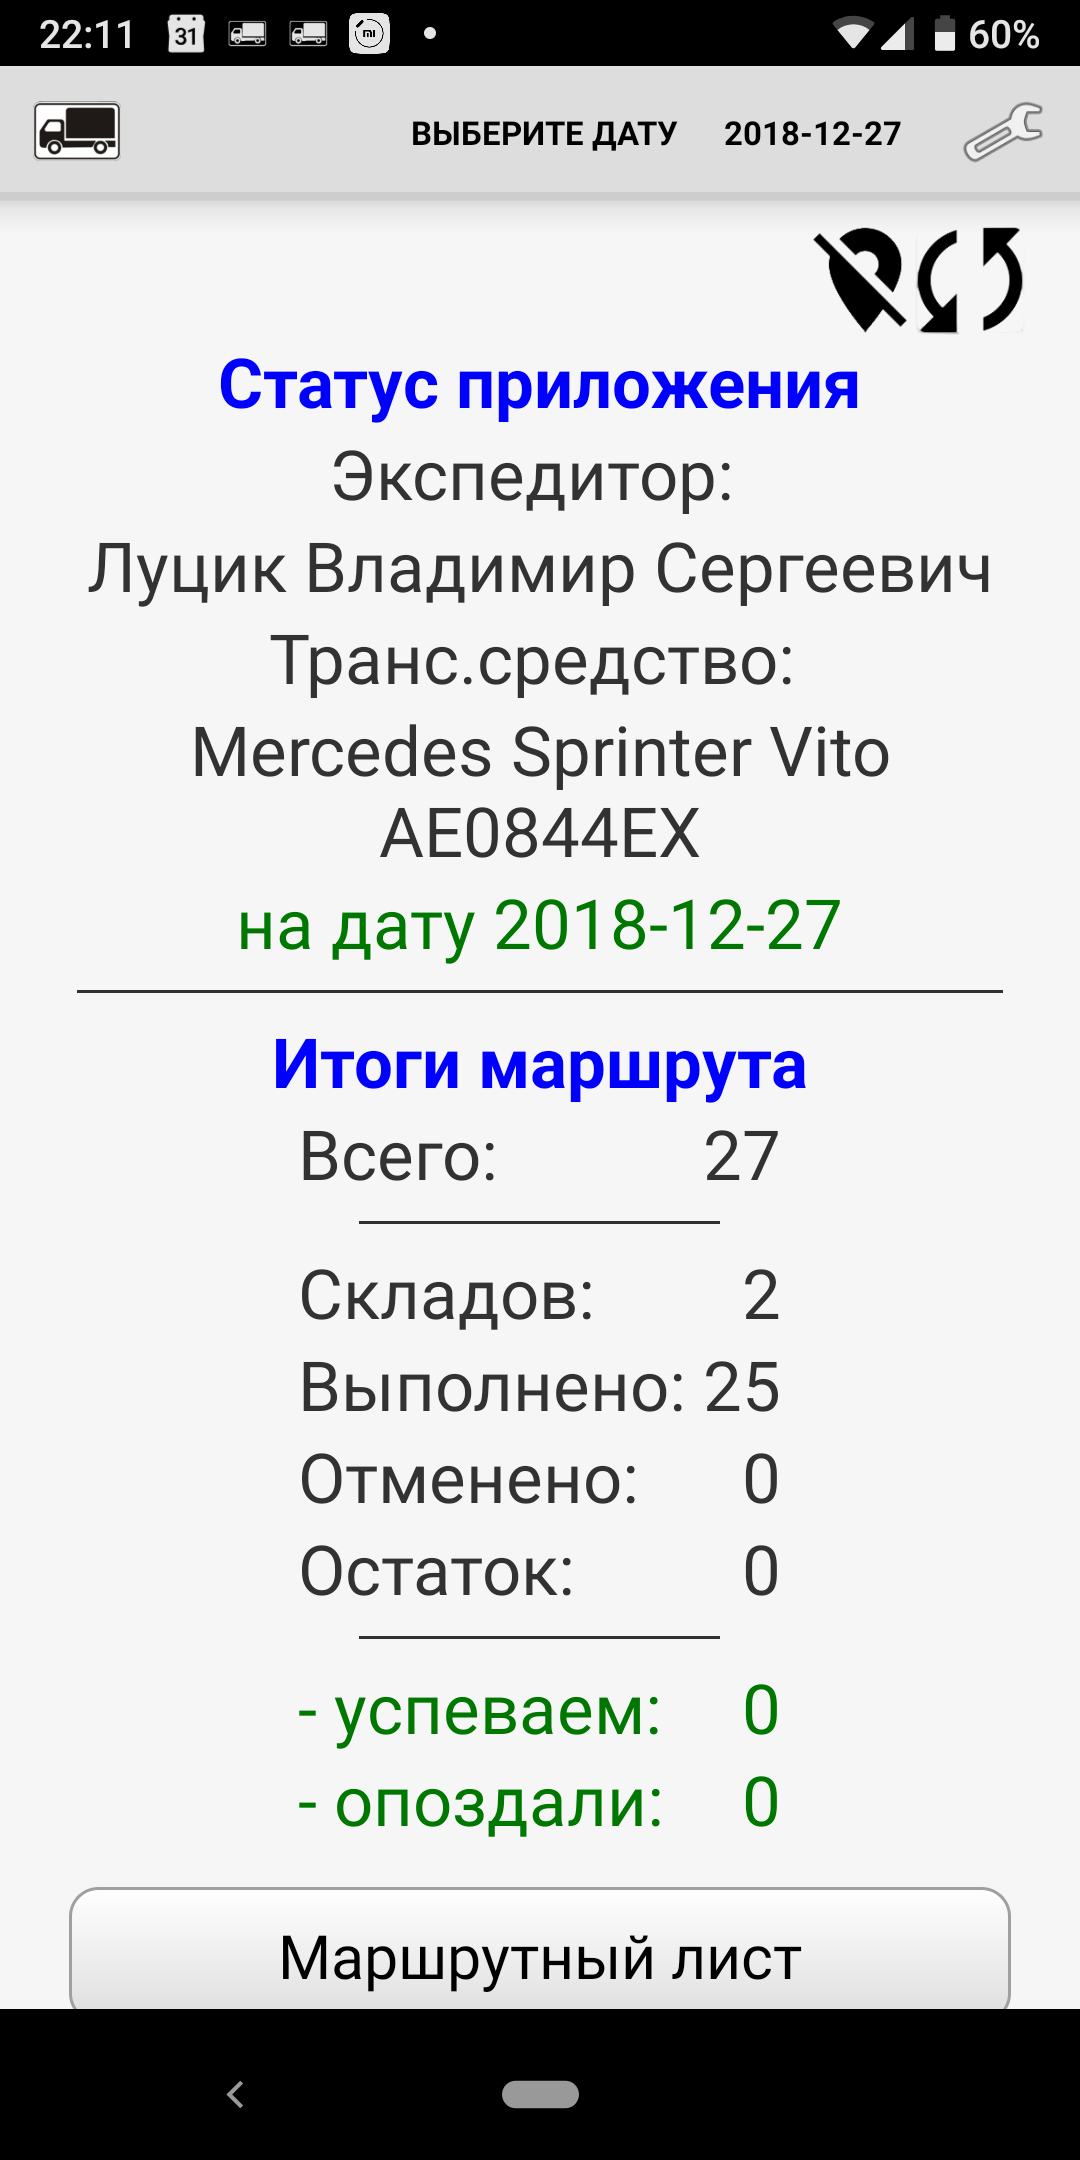
\includegraphics[width=.32\linewidth]{app-info1}}
	\hspace{0pt plus2fill}
	\subbottom[\label{img:app-info2}]{%
		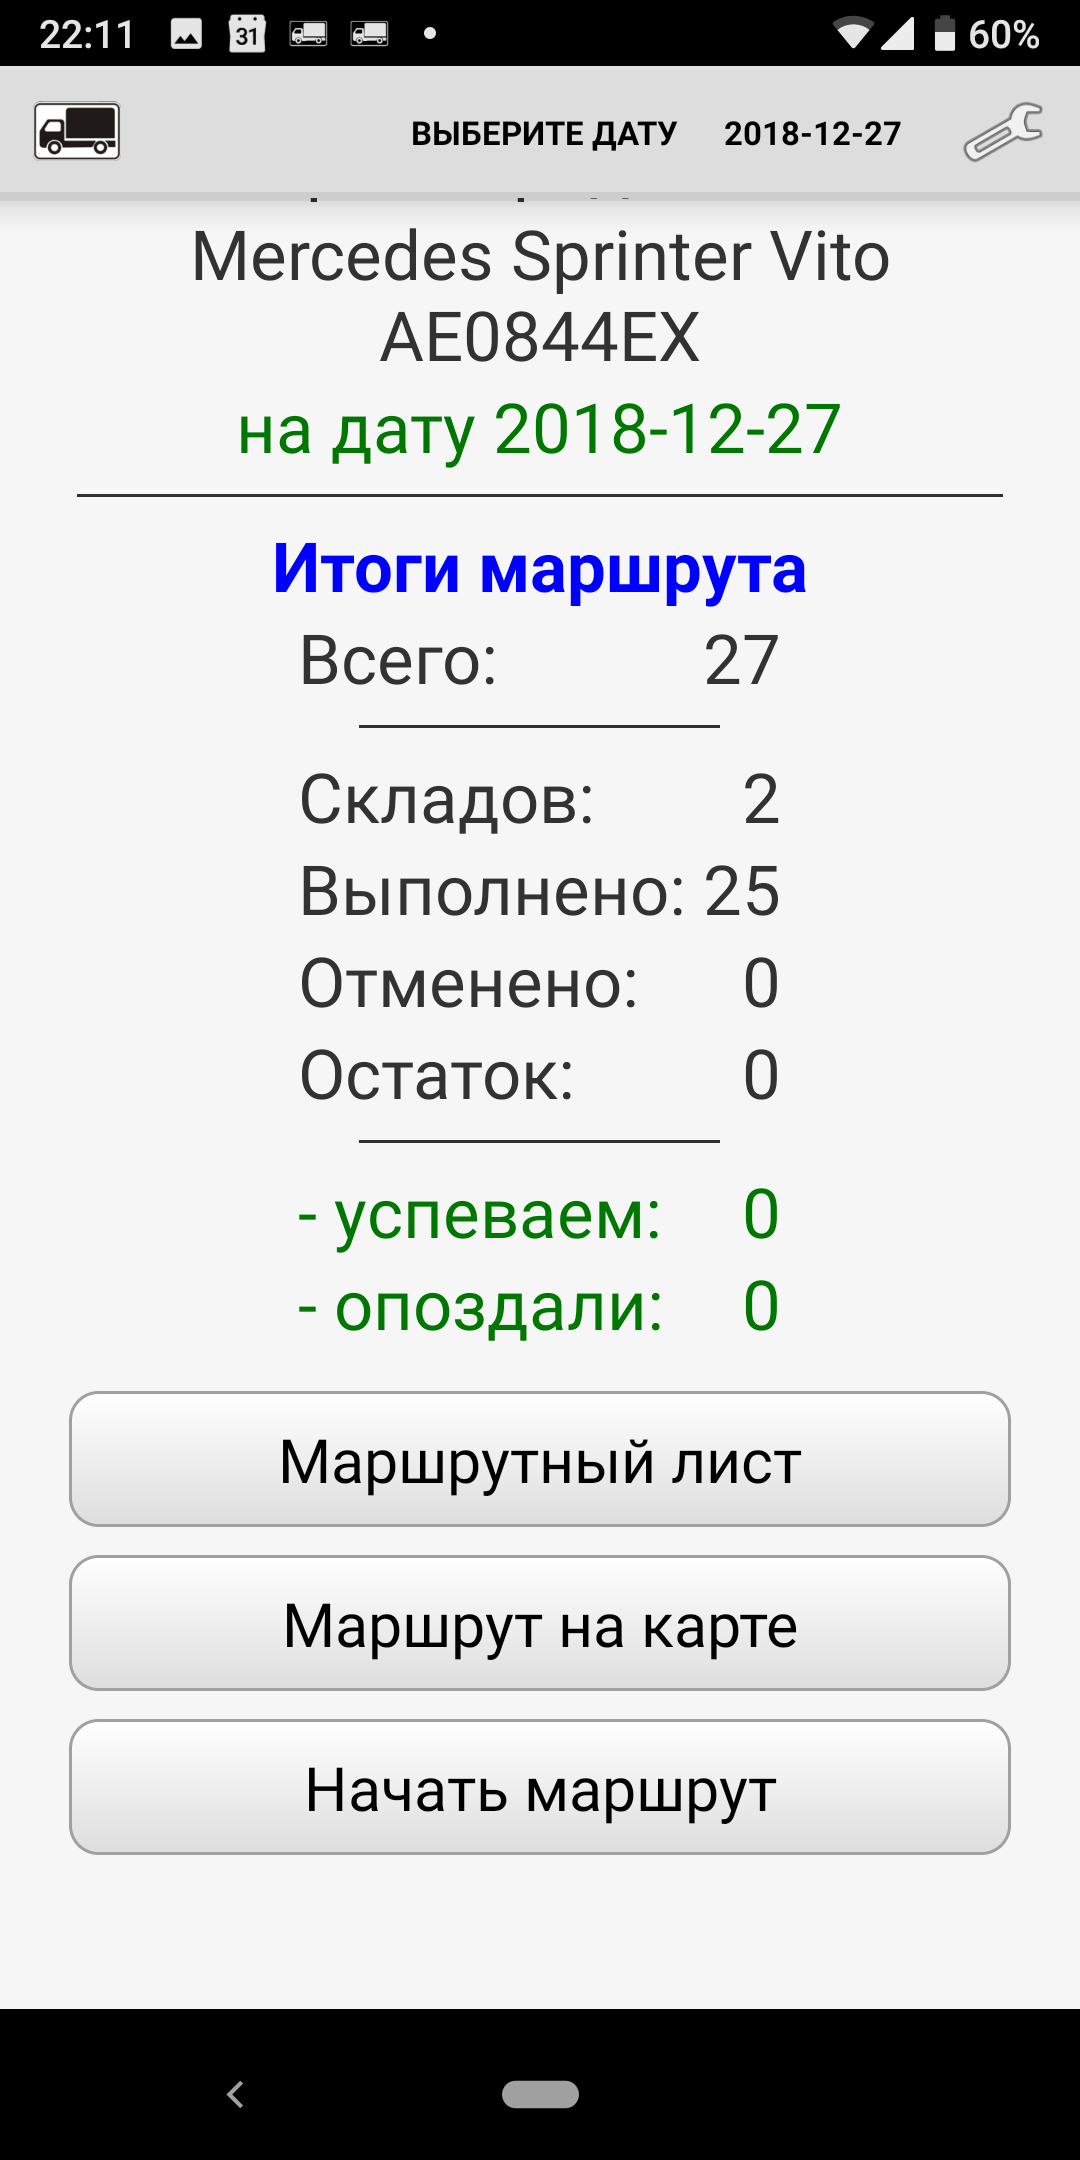
\includegraphics[width=.32\linewidth]{app-info2}}
	\hspace{0pt plus2fill}
	\subbottom[\label{img:app-info-late}]{%
		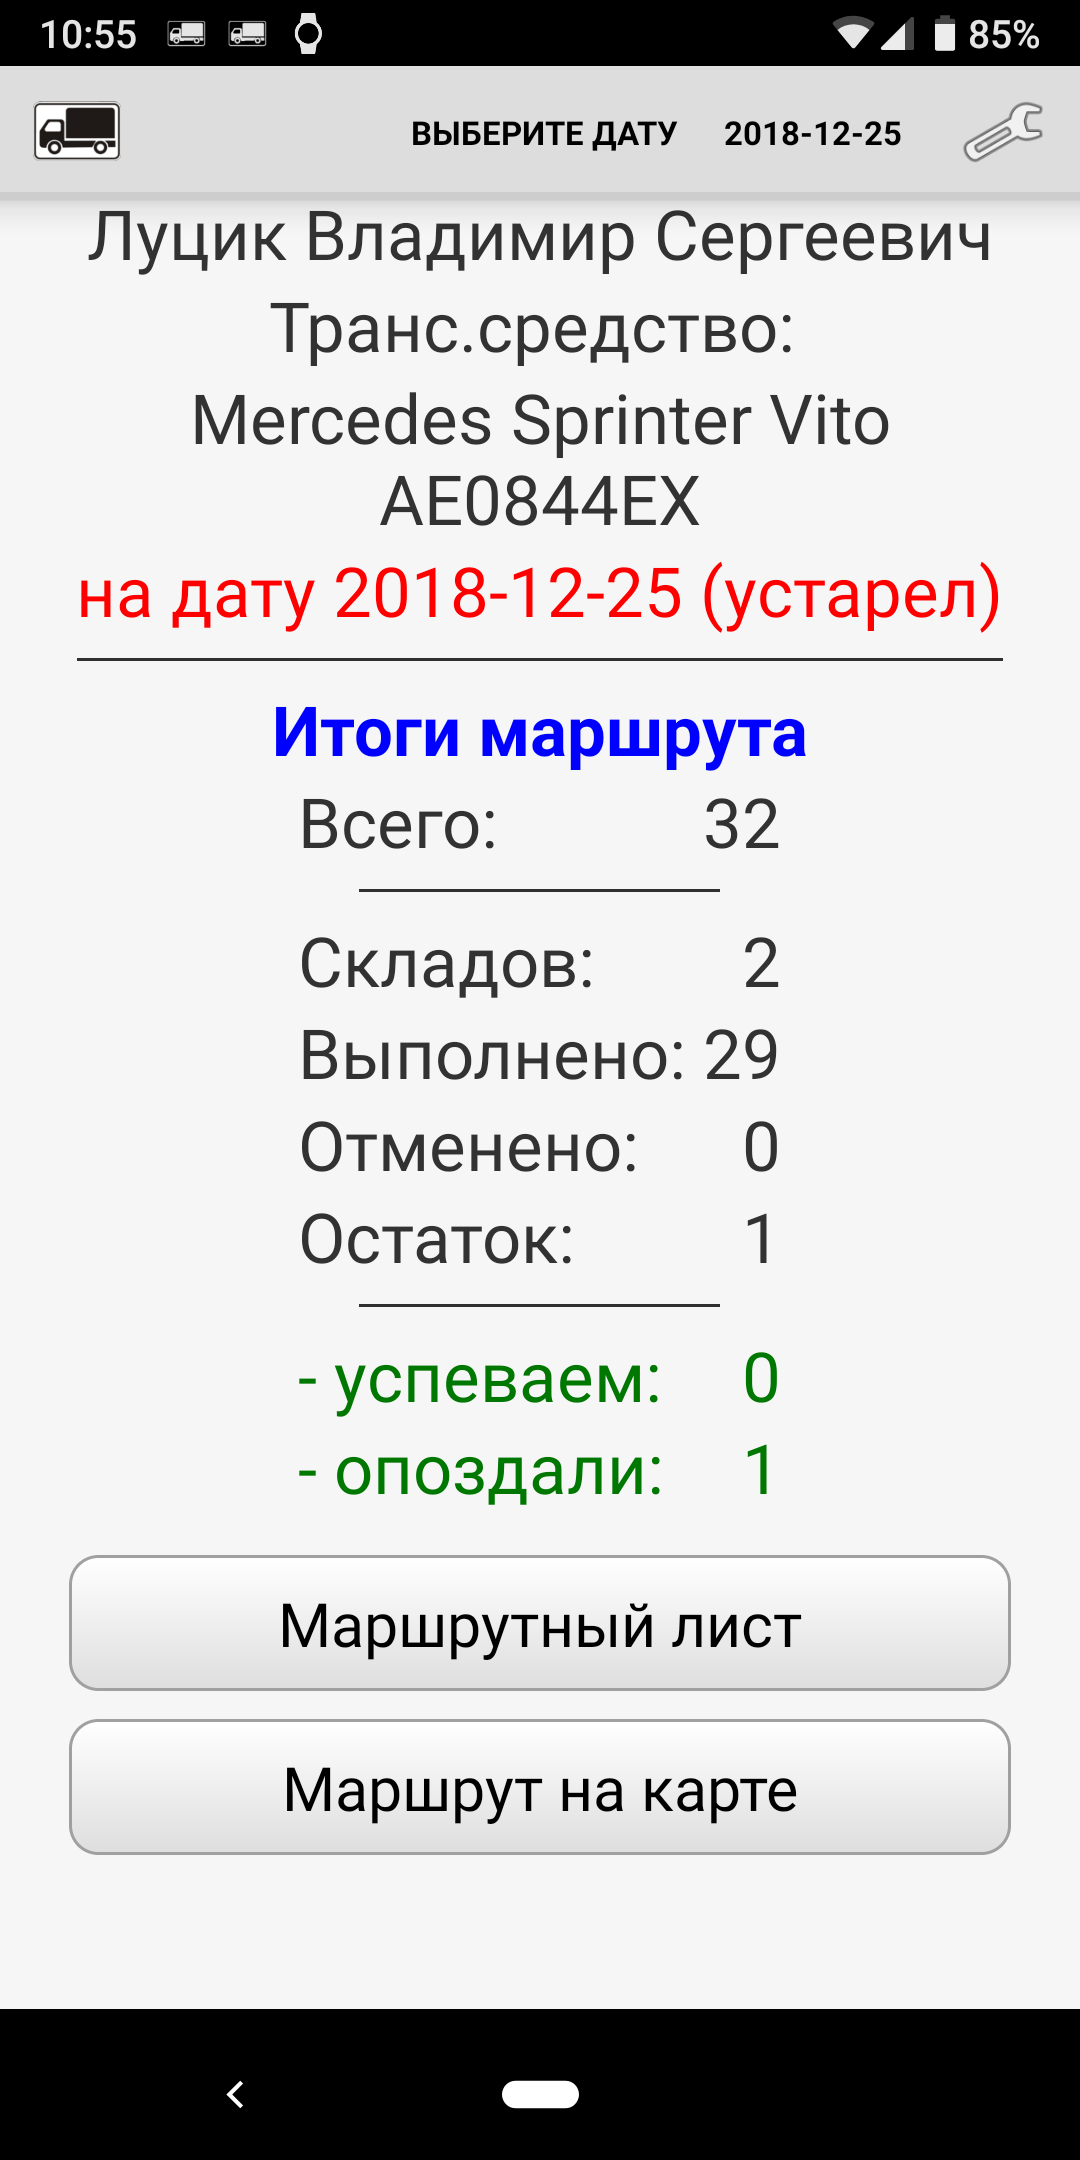
\includegraphics[width=.32\linewidth]{app-info-late}}
	\hspace{0pt plus1fill}
	\caption{Інтерфейс загальної інформації про маршрут, в тому числі з відміткою не виконаних точок (\subcaptionref{img:app-list-late})}
	\label{img:app-info}
\end{figure}
\begin{figure}
	\centering
	\hspace{0pt plus1fill}
	\subbottom[\label{img:app-list1}]{%
		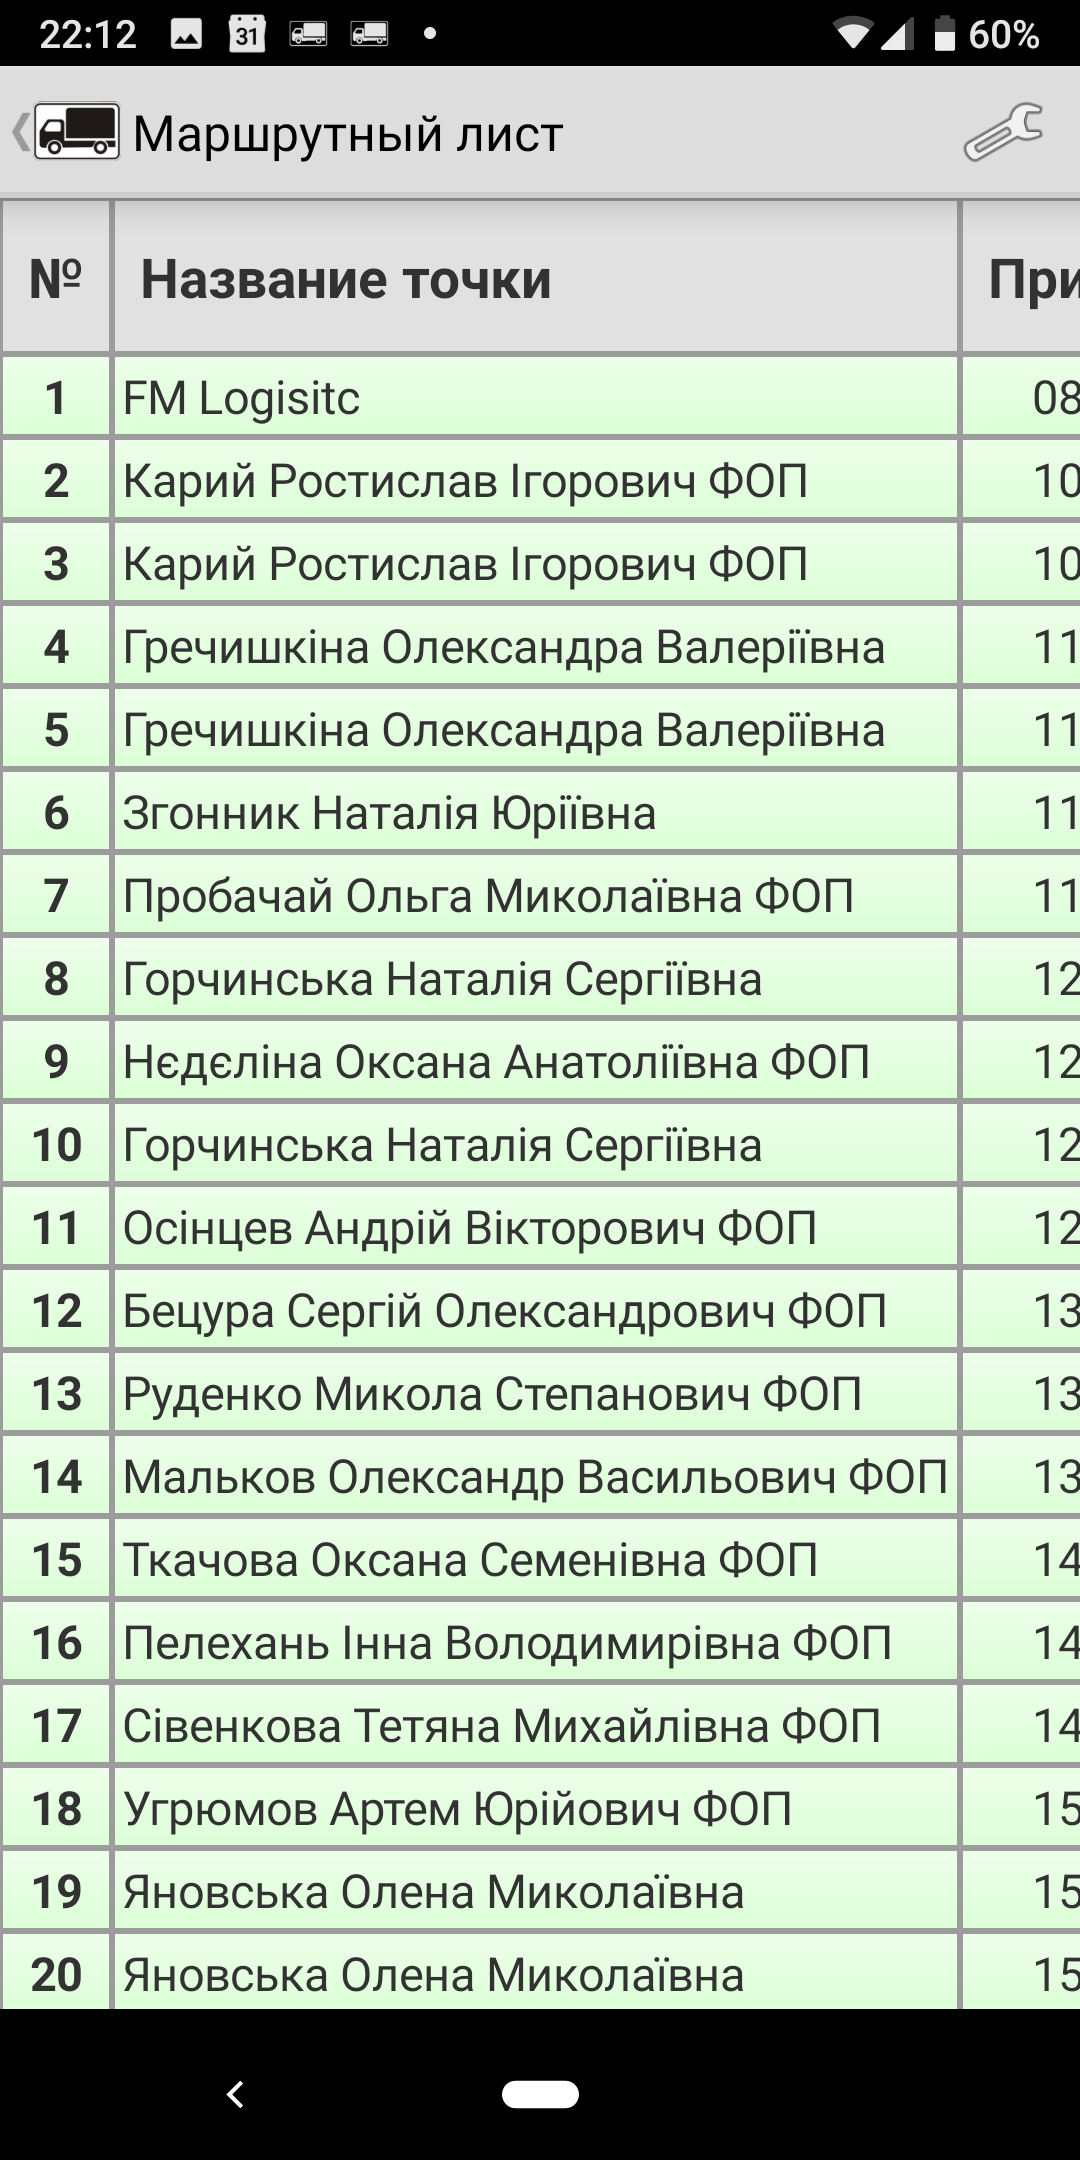
\includegraphics[width=.32\linewidth]{app-list1}}
	\hspace{0pt plus2fill}
	\subbottom[\label{img:app-list2}]{%
		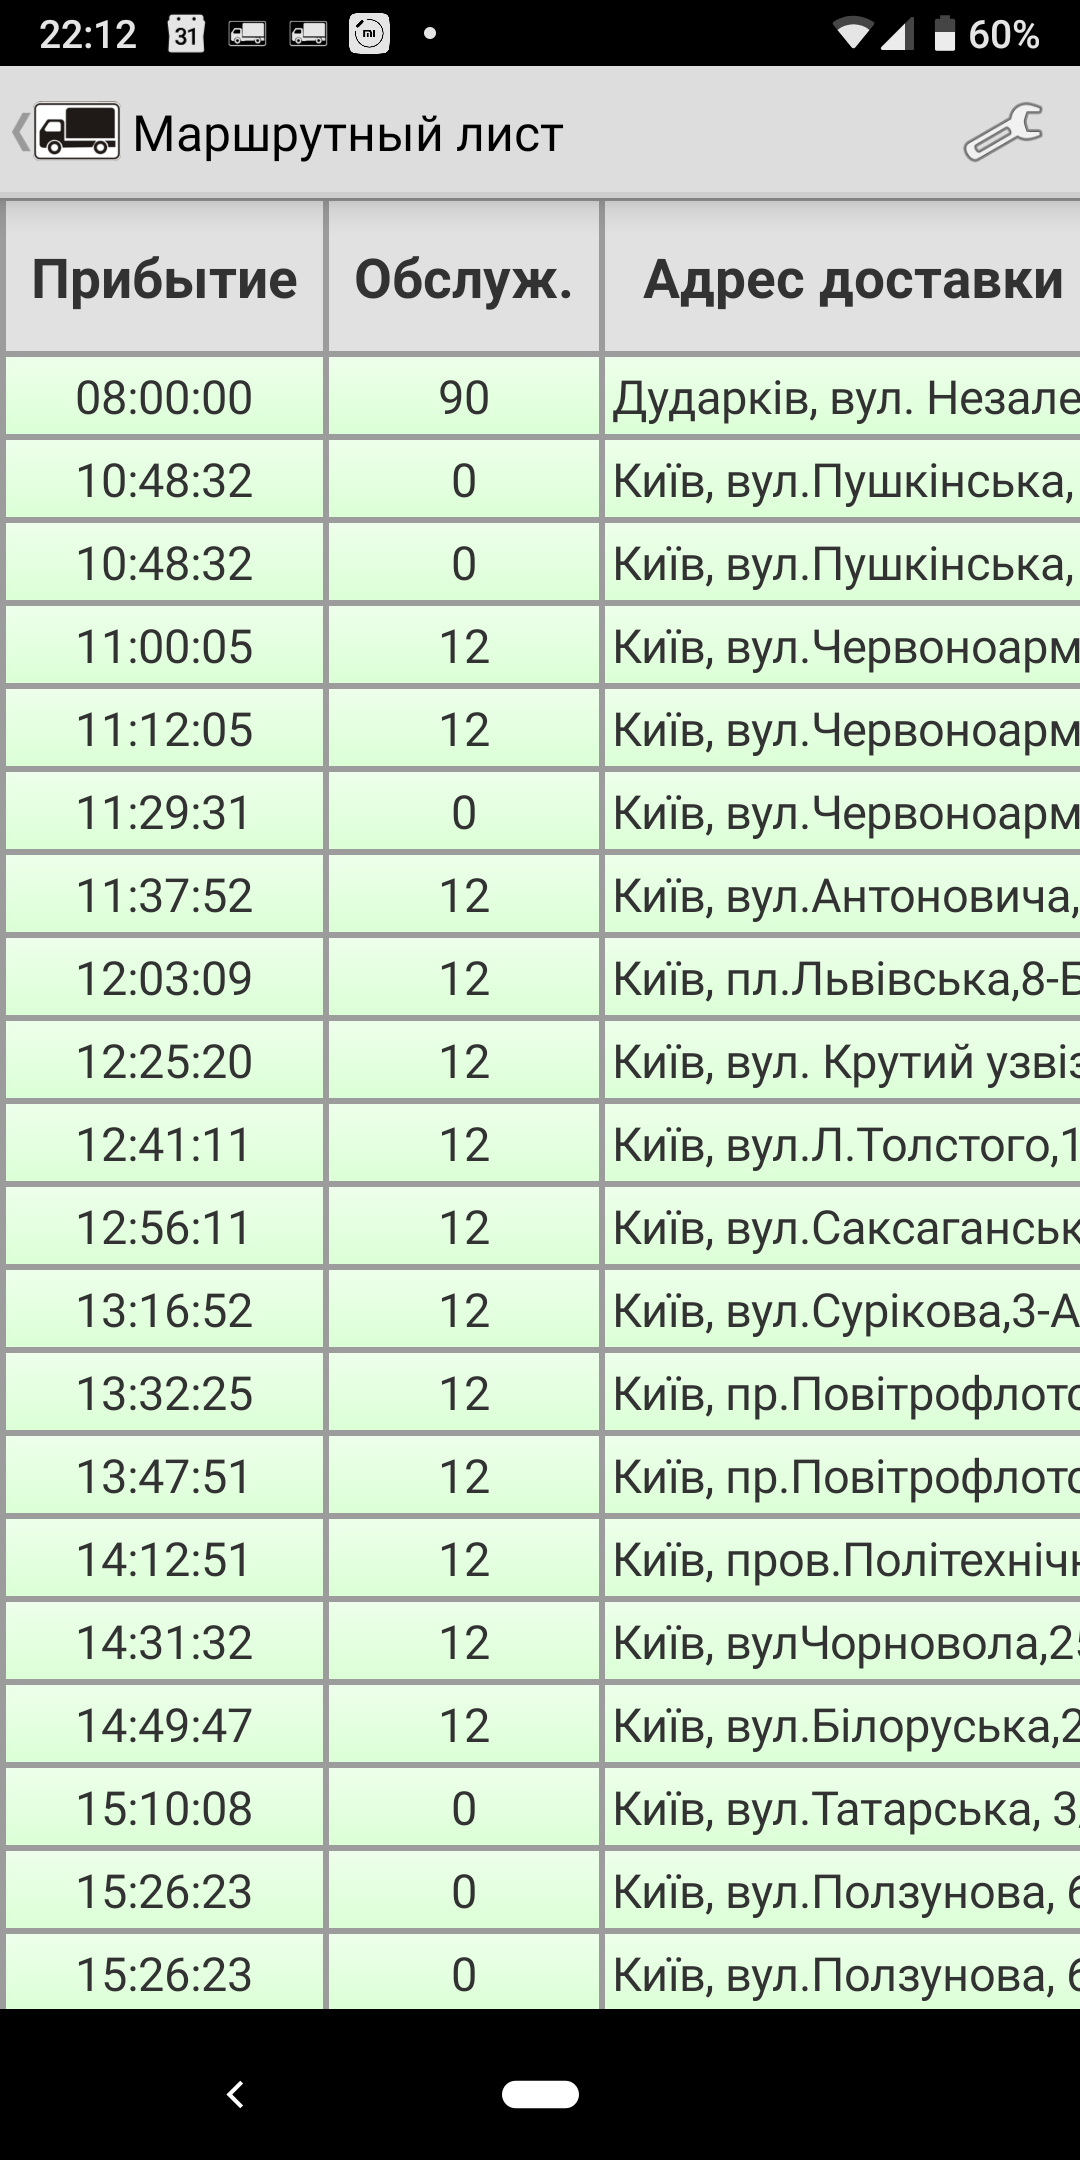
\includegraphics[width=.32\linewidth]{app-list2}}
	\hspace{0pt plus2fill}
	\subbottom[\label{img:app-list-late}]{%
		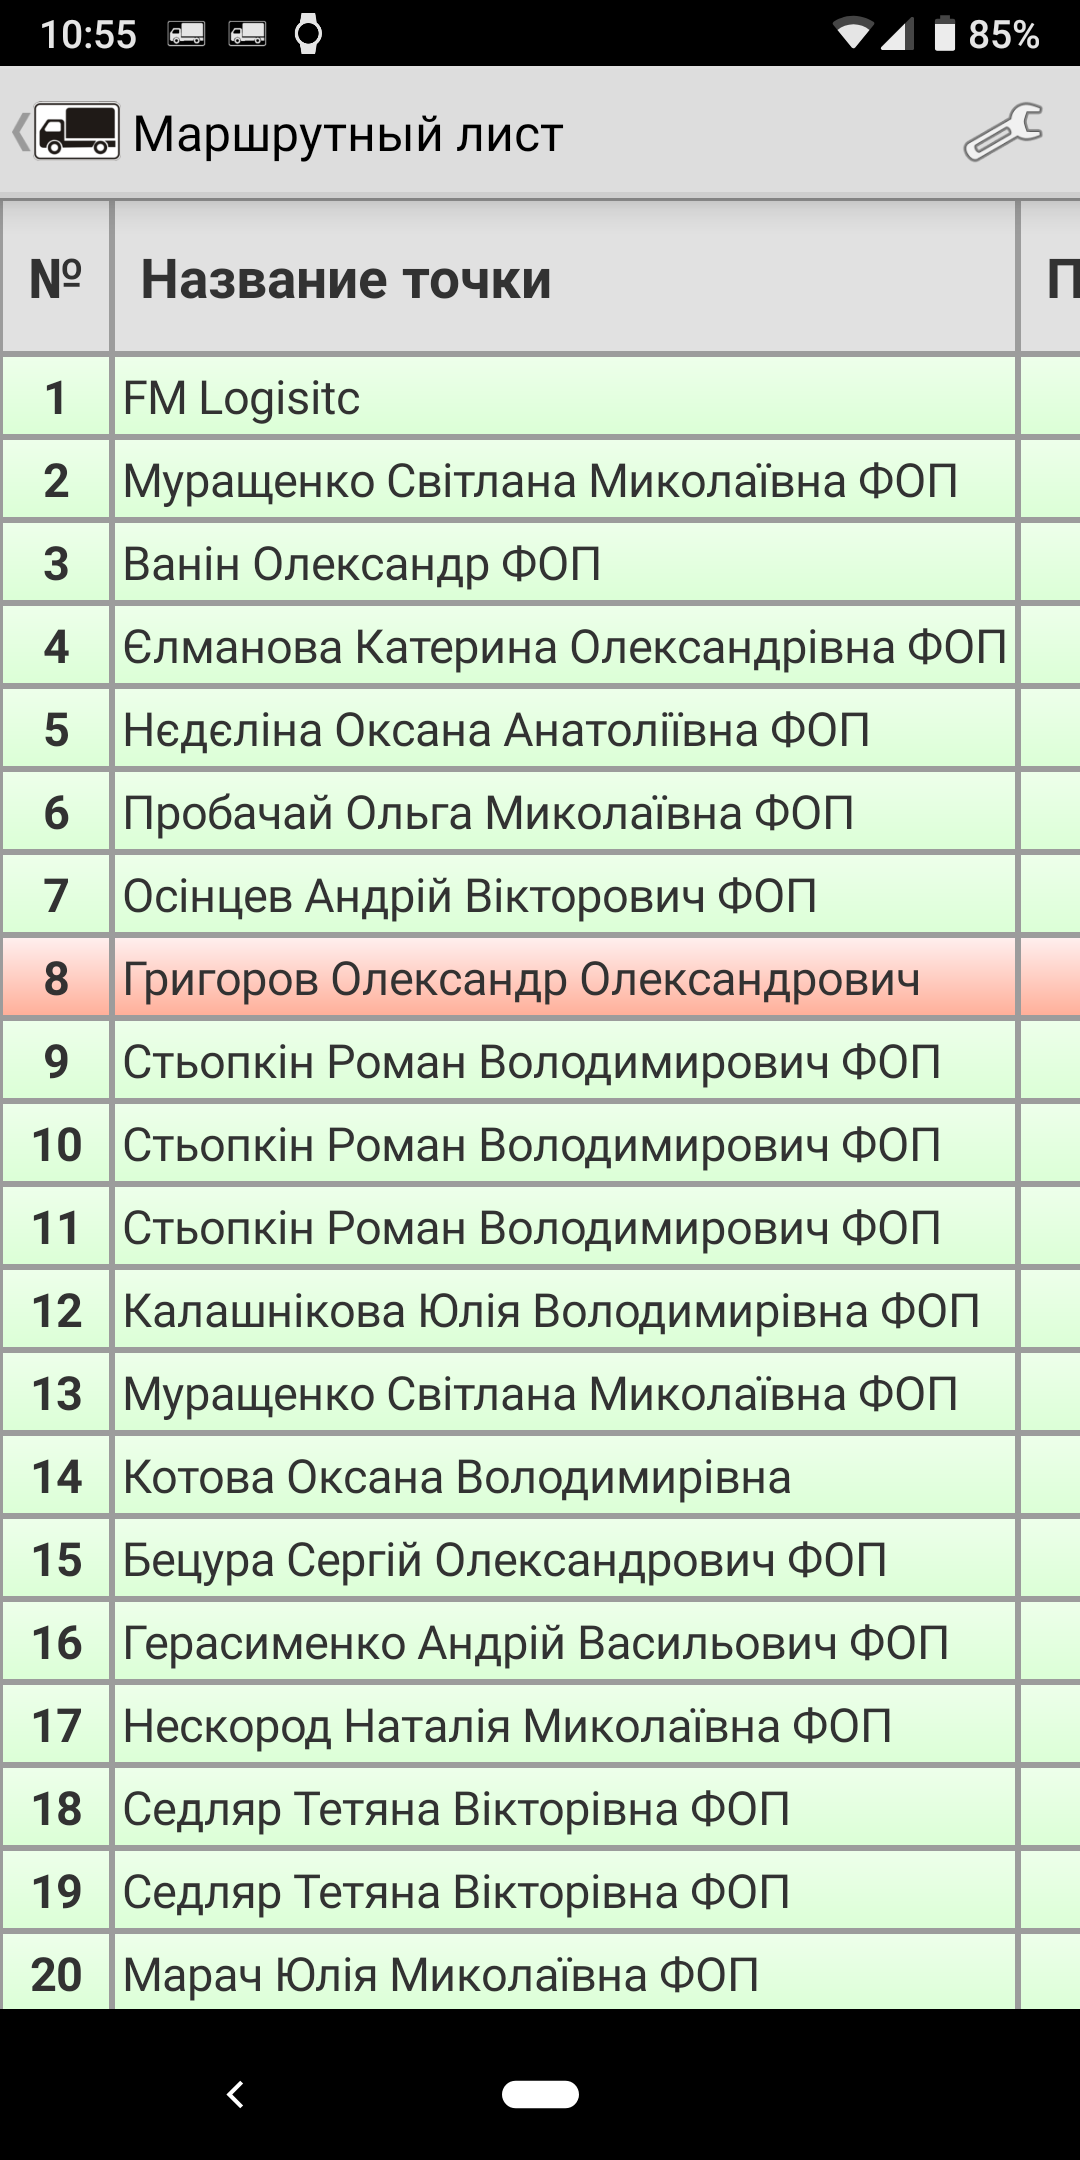
\includegraphics[width=.32\linewidth]{app-list-late}}
	\hspace{0pt plus1fill}
	\caption{Інтерфейс вікна маршрутного листа, в тому числі з відміткою не виконаної точки (\subcaptionref{img:app-list-late})}
	\label{img:app-list}
\end{figure}
\begin{figure}
	\centering
	\hspace{0pt plus1fill}
	\subbottom[\label{img:app-point}]{%
		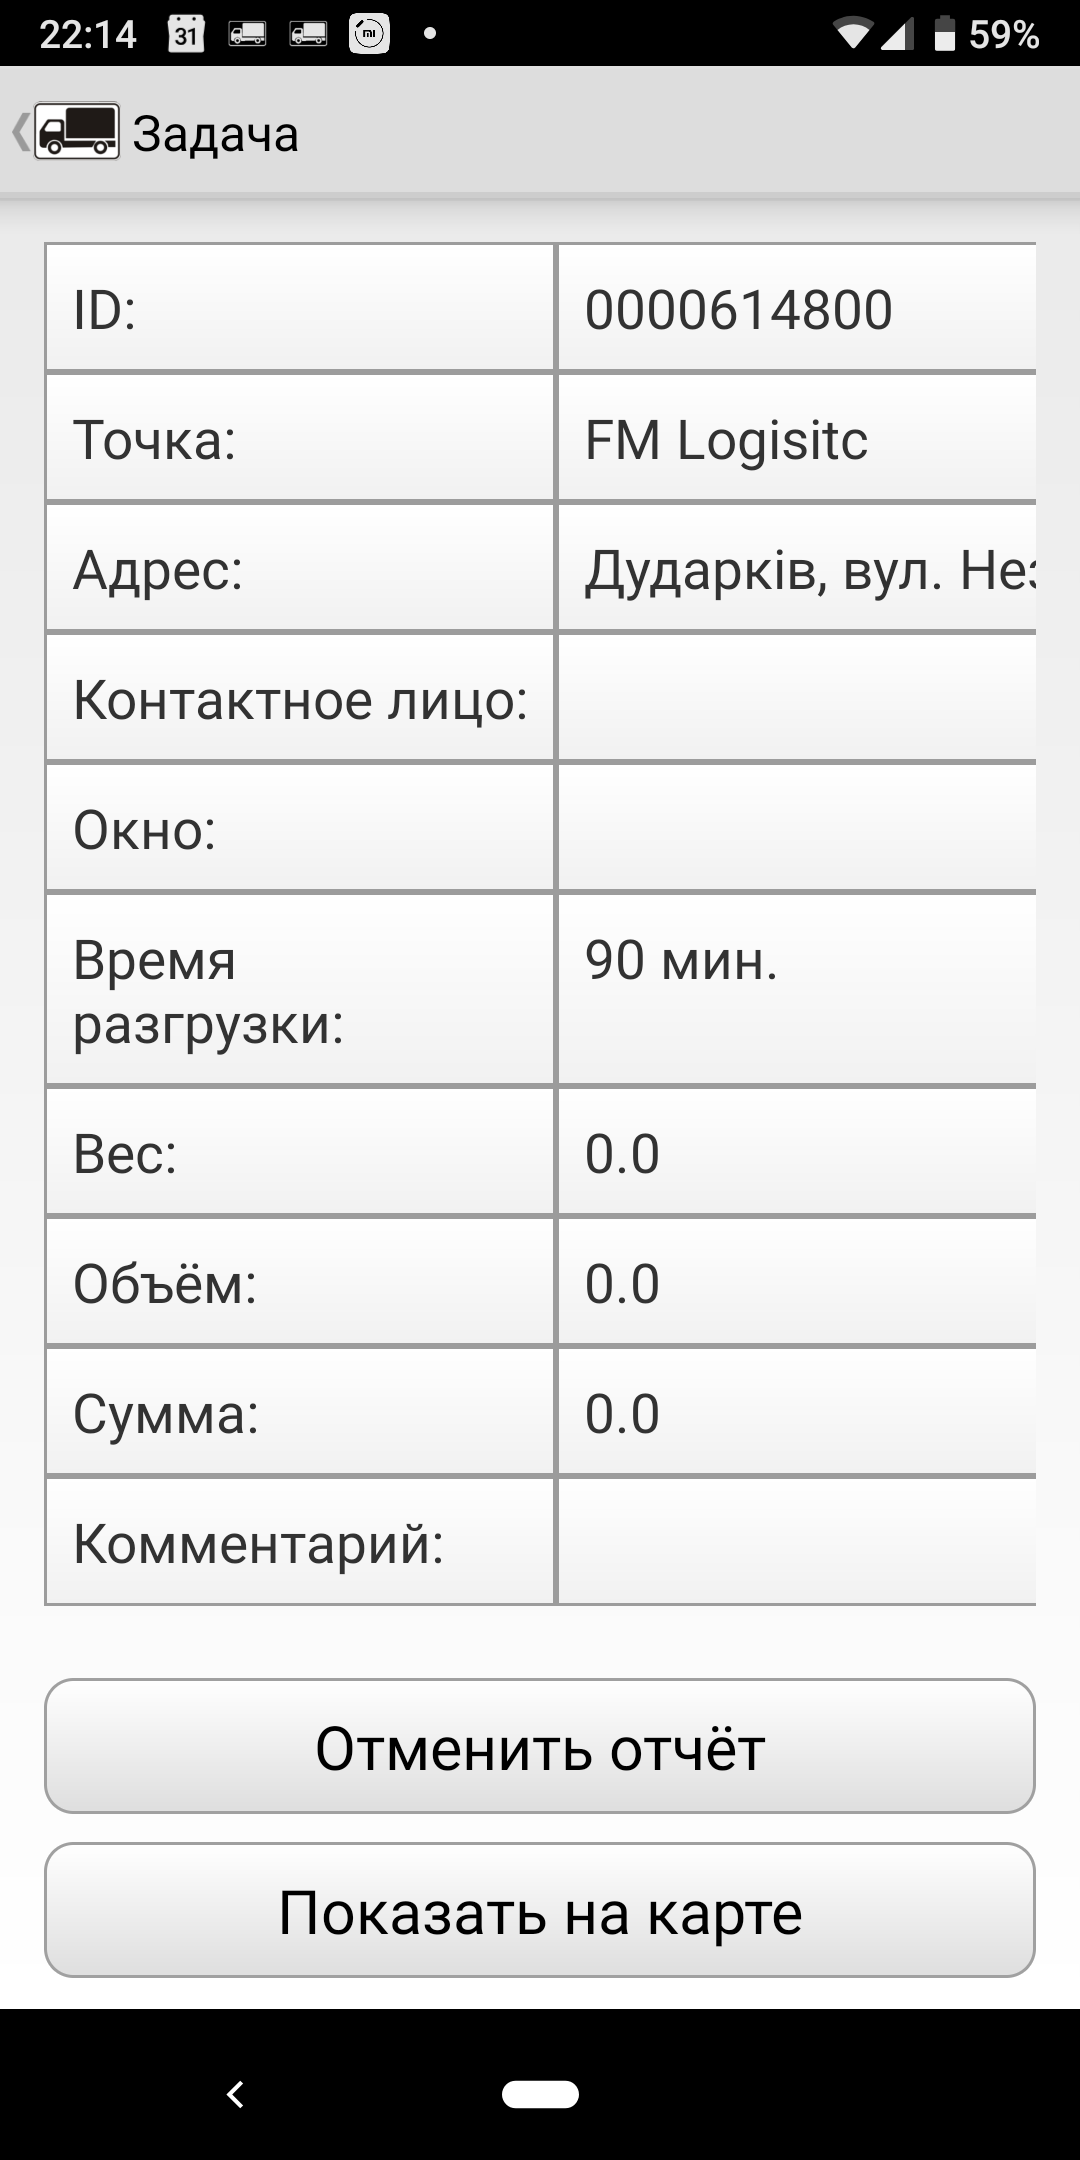
\includegraphics[width=.32\linewidth]{app-point}}
	\hspace{0pt plus2fill}
	\subbottom[\label{img:app-map}]{%
		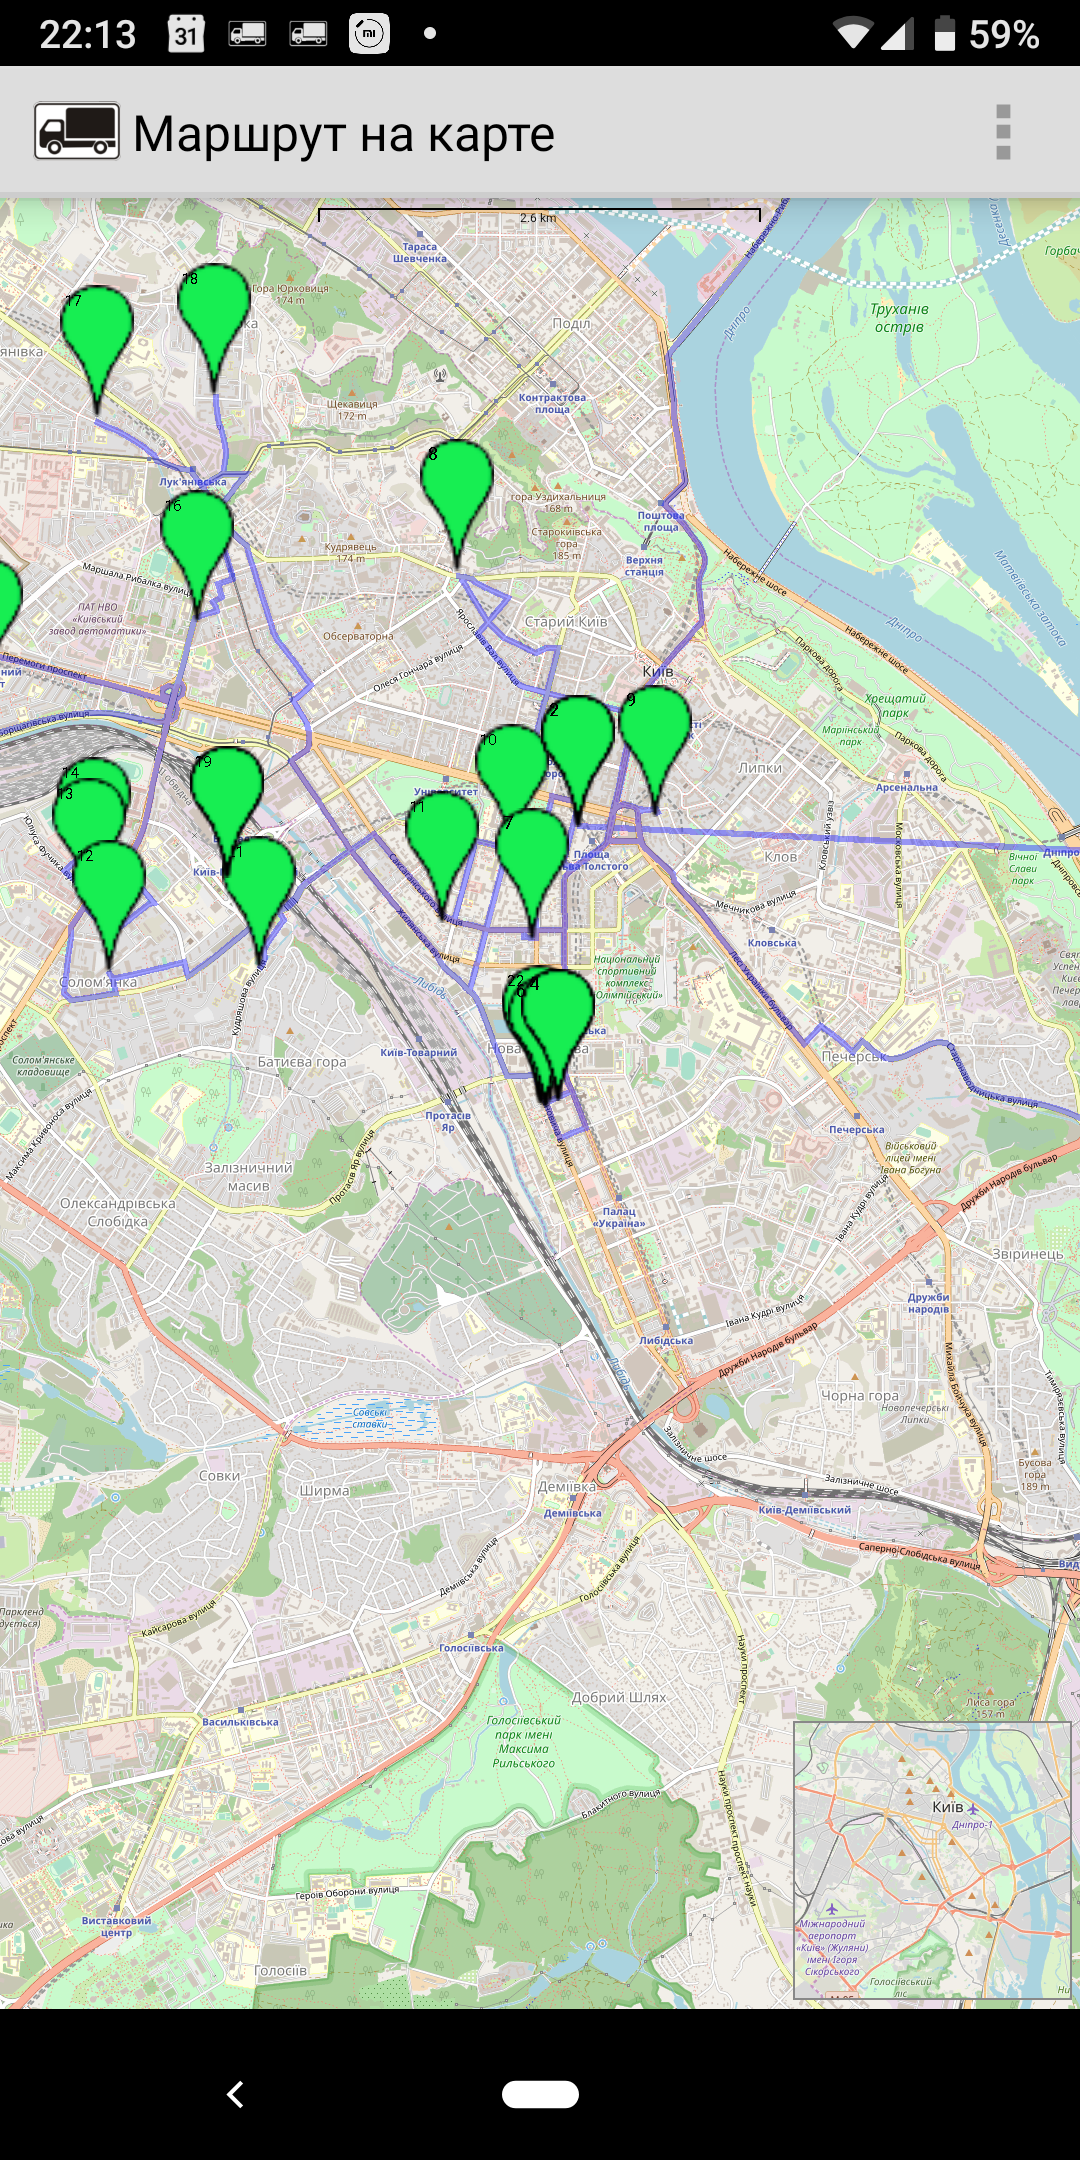
\includegraphics[width=.32\linewidth]{app-map}}
	\hspace{0pt plus2fill}
	\subbottom[\label{img:app-map-late}]{%
		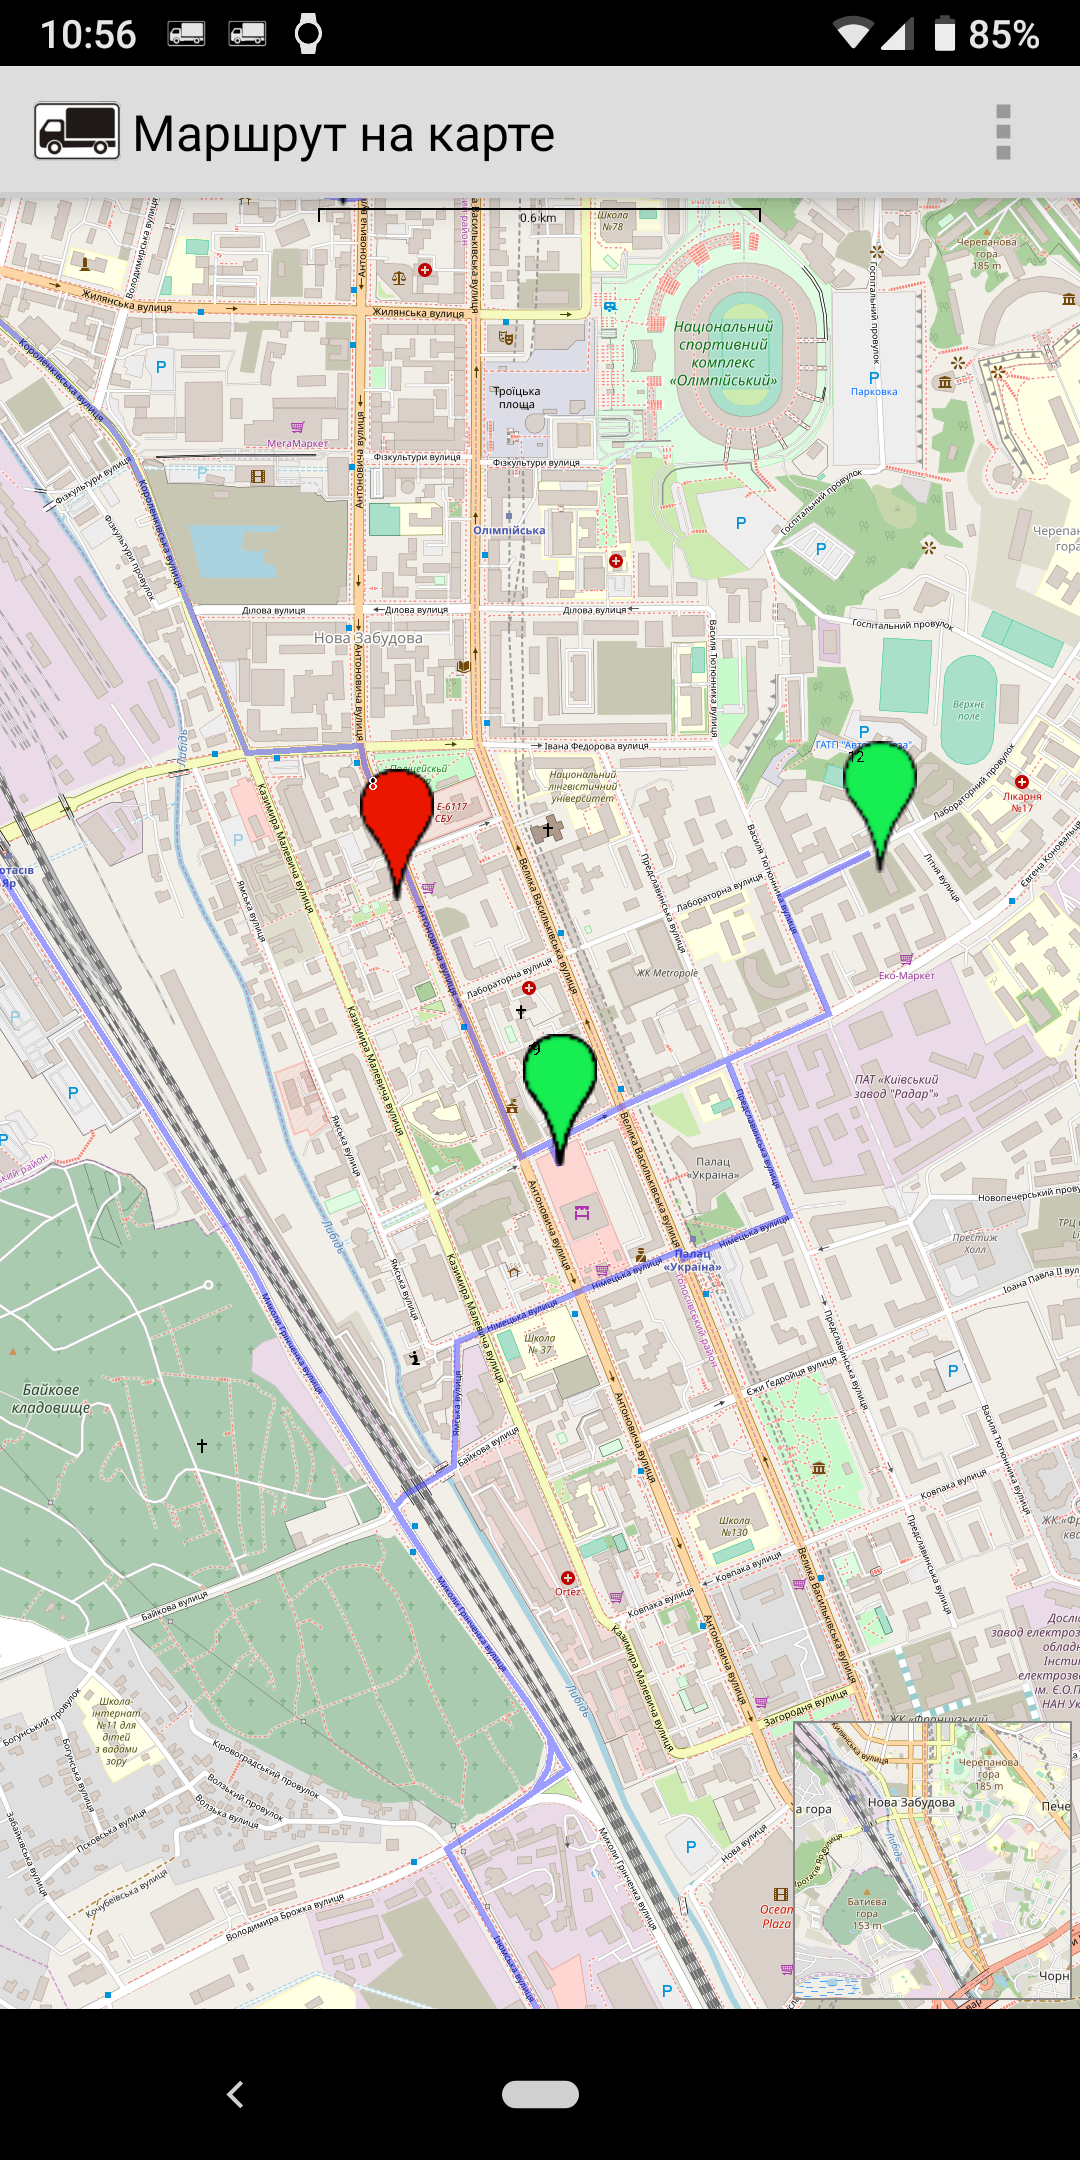
\includegraphics[width=.32\linewidth]{app-map-late}}
	\hspace{0pt plus1fill}
	\caption{Інтерфейс інформації про точку (\subcaptionref{img:app-point}) та мапи маршруту (\subcaptionref{img:app-map}), в тому числі з відміткою не виконаних точок (\subcaptionref{img:app-map-late})}
	\label{img:app-point-map}
\end{figure}
\begin{mytable}[ht]{ | c | c | c | c | c | c | c | }%
	{Детальний розподіл за дикторами та пристроями голосових даних зібраних на першому етапі моделювання}%
	{\label{tbl:data1_distribution}}%
	{
		\specialcell{3cm}{Диктор} & 
		\specialcell{3cm}{Пристрій} & 
		\specialcell{3cm}{Стать} & 
		\specialcell{3cm}{Кількість \\ записів} & 
		\specialcell{3cm}{Кількість \\ реакцій} &
		\specialcell{3cm}{Кількість \\ варіантів \\ стимулів} & 
		\specialcell{3cm}{Кількість \\ записів \\ реакції часу}}
	
	1 & 1 & жін. & 109 & 64 & 92 & 22 \\
	\hline
	2 & 1 & жін. & 105 & 64 & 96 & 22 \\
	\hline
	3 & 1 & жін. & 100 & 64 & 96 & 21 \\
	\hline
	4 & 1 & жін. & 97 & 64 & 93 & 22 \\
	\hline
	5 & 1 & жін. & 96 & 64 & 93 & 22 \\
	\hline
	6 & 1 & жін. & 95 & 64 & 94 & 22 \\
	\hline
	7 & 1 & жін. & 95 & 64 & 95 & 23 \\
	\hline
	8 & 1 & жін. & 95 & 62 & 90 & 21 \\
	\hline
	9 & 1 & жін. & 90 & 62 & 89 & 22 \\
	\hline
	10 & 1 & жін. & 79 & 58 & 79 & 23 \\
	\hline
	11 & 1 & чол. & 196 & 64 & 96 & 44 \\
	\hline
	12 & 1 & чол. & 101 & 64 & 94 & 25 \\
	\hline
	13 & 1 & чол. & 96 & 64 & 92 & 22 \\
	\hline
	14 & 1 & чол. & 98 & 63 & 95 & 21 \\
	\hline
	15 & 1 & чол. & 89 & 63 & 85 & 22 \\
	\hline
	16 & 1 & чол. & 98 & 62 & 90 & 21 \\
	\hline
	17 & 1 & чол. & 64 & 48 & 62 & 22 \\
	\hline
	18 & 1 & чол. & 30 & 25 & 30 & 0 \\
	\hline
	19 & 1 & чол. & 23 & 16 & 22 & 0 \\
	\hline
	20 & 1 & чол. & 23 & 9 & 19 & 0 \\
	\hline
	21 & 2 & жін. & 97 & 64 & 94 & 22 \\
	\hline
	22 & 3 & чол. & 96 & 64 & 96 & 22 \\
	\hline
	23 & 4 & чол. & 99 & 64 & 96 & 24 \\
	
\end{mytable}%
\begin{mytable}[ht]{ | c | c | c | c | c | c | }%
	{Результати моделювання першого набору даних використовуючи ІРС з послідовностями розміром 1--3}%
	{\label{tbl:total_data1_irs13}}%
	{
		\specialcell{3cm}{№ Контексту} & 
		\specialcell{3cm}{Точність \\ розпізнання} & 
		\specialcell{3cm}{Середня \\ прецизійність} & 
		\specialcell{3cm}{Середня \\ повнота} & 
		\specialcell{3cm}{Середня \\ F-міра} & 
		\specialcell{3cm}{Кількість}}	
	
	1 & 0.677 & 0.450 & 0.445 & 0.447 & 124 \\
\hline
2 & 0.456 & 0.559 & 0.663 & 0.408 & 513 \\
\hline
3 & 0.387 & 0.055 & 0.143 & 0.080 & 217 \\
\hline
4 & 0.375 & 0.217 & 0.271 & 0.171 & 104 \\
\hline
5 & 0.339 & 0.108 & 0.184 & 0.111 & 183 \\
\hline
6 & 0.397 & 0.198 & 0.252 & 0.222 & 209 \\
\hline
7 & 0.206 & 0.021 & 0.098 & 0.034 & 233 \\
\hline
8 & 0.346 & 0.182 & 0.179 & 0.107 & 217 \\
\hline
9 & 0.344 & 0.144 & 0.225 & 0.141 & 131 \\
\hline
10 & 0.349 & 0.489 & 0.255 & 0.194 & 126 \\
\hline
11 & 0.268 & 0.099 & 0.145 & 0.114 & 239 \\
\hline
12 & 0.264 & 0.303 & 0.250 & 0.238 & 201 \\
\hline
13 & 0.450 & 0.361 & 0.259 & 0.182 & 171 \\
\hline
14 & 0.439 & 0.551 & 0.432 & 0.432 & 139 \\
\hline
15 & 0.302 & 0.547 & 0.210 & 0.152 & 159 \\
\hline
16 & 0.478 & 0.539 & 0.470 & 0.450 & 115 \\
\hline
17 & 0.271 & 0.261 & 0.263 & 0.248 & 155 \\
\hline
18 & 0.418 & 0.482 & 0.411 & 0.407 & 110 \\
\hline
19 & 0.471 & 0.650 & 0.458 & 0.462 & 87 \\
\hline
\specialcell{3cm}{По всій \\ вибірці} & 0.044 & 0.027 & 0.017 & 0.009 & 2069 \\
\hline
\specialcell{3cm}{Тестовий \\ контекст} & 0.485 & 0.162 & 0.333 & 0.218 & 101 \\
\end{mytable}
\begin{mytable}[ht]{ | c | c | c | c | c | c | }%
	{Результати моделювання першого набору даних використовуючи ІРС з послідовностями розміром 2--4}%
	{\label{tbl:total_data1_irs24}}%
	{
		\specialcell{3cm}{№ Контексту} & 
		\specialcell{3cm}{Точність \\ розпізнання} & 
		\specialcell{3cm}{Середня \\ прецизійність} & 
		\specialcell{3cm}{Середня \\ повнота} & 
		\specialcell{3cm}{Середня \\ F-міра} & 
		\specialcell{3cm}{Кількість}}	
	
	1 & 0.710 & 0.503 & 0.442 & 0.459 & 124 \\
\hline
2 & 0.895 & 0.465 & 0.478 & 0.471 & 513 \\
\hline
3 & 0.382 & 0.048 & 0.124 & 0.069 & 217 \\
\hline
4 & 0.558 & 0.740 & 0.480 & 0.484 & 104 \\
\hline
5 & 0.415 & 0.434 & 0.259 & 0.225 & 183 \\
\hline
6 & 0.565 & 0.282 & 0.359 & 0.316 & 209 \\
\hline
7 & 0.232 & 0.388 & 0.127 & 0.089 & 233 \\
\hline
8 & 0.373 & 0.410 & 0.207 & 0.157 & 217 \\
\hline
9 & 0.527 & 0.737 & 0.437 & 0.449 & 131 \\
\hline
10 & 0.532 & 0.773 & 0.468 & 0.486 & 126 \\
\hline
11 & 0.515 & 0.207 & 0.282 & 0.238 & 239 \\
\hline
12 & 0.488 & 0.510 & 0.469 & 0.452 & 201 \\
\hline
13 & 0.485 & 0.448 & 0.303 & 0.283 & 171 \\
\hline
14 & 0.633 & 0.703 & 0.625 & 0.625 & 139 \\
\hline
15 & 0.453 & 0.480 & 0.329 & 0.333 & 159 \\
\hline
16 & 0.583 & 0.661 & 0.574 & 0.550 & 115 \\
\hline
17 & 0.387 & 0.473 & 0.378 & 0.374 & 155 \\
\hline
18 & 0.582 & 0.672 & 0.576 & 0.583 & 110 \\
\hline
19 & 0.655 & 0.728 & 0.650 & 0.642 & 87 \\
\hline
\specialcell{3cm}{По всій \\ вибірці} & 0.122 & 0.061 & 0.048 & 0.027 & 2069 \\
\hline
\specialcell{3cm}{Тестовий \\ контекст} & 0.475 & 0.160 & 0.327 & 0.215 & 101 \\
\end{mytable}
\begin{mytable}[ht]{ | c | c | c | c | c | c | }%
	{Результати моделювання першого набору даних використовуючи ЗНМ з послідовностями розміром 2--4}%
	{\label{tbl:total_data1_cnn}}%
	{
		\specialcell{3cm}{№ Контексту} & 
		\specialcell{3cm}{Точність \\ розпізнання} & 
		\specialcell{3cm}{Середня \\ прецизійність} & 
		\specialcell{3cm}{Середня \\ повнота} & 
		\specialcell{3cm}{Середня \\ F-міра} & 
		\specialcell{3cm}{Кількість}}	
	
	1 & 0.879 & 0.880 & 0.863 & 0.870 & 124 \\
\hline
2 & 0.957 & 0.933 & 0.799 & 0.851 & 513 \\
\hline
3 & 0.820 & 0.870 & 0.777 & 0.813 & 217 \\
\hline
4 & 0.846 & 0.857 & 0.829 & 0.837 & 104 \\
\hline
5 & 0.798 & 0.814 & 0.734 & 0.754 & 183 \\
\hline
6 & 0.852 & 0.851 & 0.789 & 0.814 & 209 \\
\hline
7 & 0.785 & 0.808 & 0.773 & 0.785 & 233 \\
\hline
8 & 0.871 & 0.895 & 0.847 & 0.867 & 217 \\
\hline
9 & 0.863 & 0.871 & 0.836 & 0.847 & 131 \\
\hline
10 & 0.825 & 0.841 & 0.818 & 0.819 & 126 \\
\hline
11 & 0.908 & 0.922 & 0.850 & 0.878 & 239 \\
\hline
12 & 0.846 & 0.852 & 0.849 & 0.847 & 201 \\
\hline
13 & 0.848 & 0.860 & 0.842 & 0.849 & 171 \\
\hline
14 & 0.842 & 0.851 & 0.838 & 0.838 & 139 \\
\hline
15 & 0.849 & 0.842 & 0.829 & 0.834 & 159 \\
\hline
16 & 0.817 & 0.826 & 0.814 & 0.814 & 115 \\
\hline
17 & 0.723 & 0.729 & 0.723 & 0.720 & 155 \\
\hline
18 & 0.836 & 0.842 & 0.837 & 0.835 & 110 \\
\hline
19 & 0.862 & 0.871 & 0.863 & 0.856 & 87 \\
\hline
\specialcell{3cm}{По всій \\ вибірці} & 0.652 & 0.679 & 0.622 & 0.640 & 2069 \\
\hline
\specialcell{3cm}{Тестовий \\ контекст} & 0.891 & 0.915 & 0.871 & 0.888 & 101 \\
\end{mytable}
\begin{figure}[!t]
	\centering
	\subbottom[Метод ІРС розміром 1--3 \label{img:accuracy_distribution_data1_irs13}]{%
		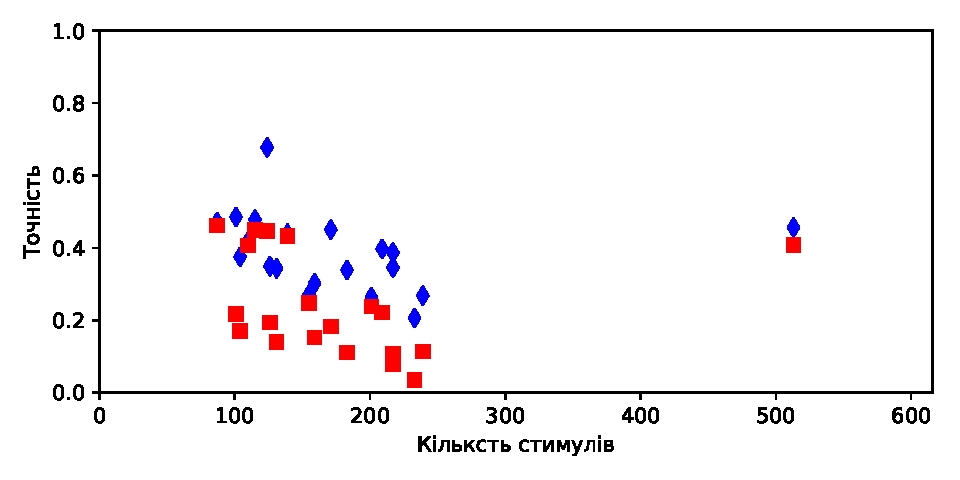
\includegraphics[width=.7\linewidth]{accuracy_distribution_data1_irs13}}
	\\
	\subbottom[Метод ІРС розміром 2--4 \label{img:accuracy_distribution_data1_irs24}]{%
		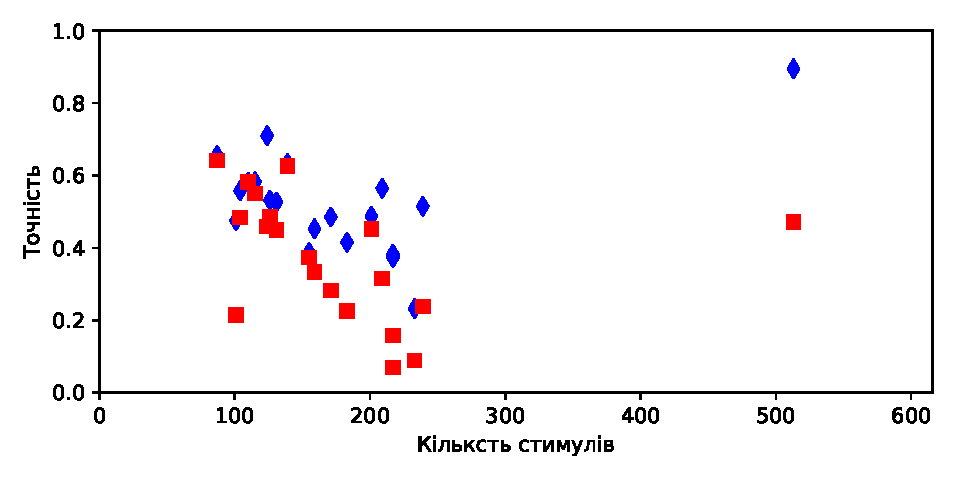
\includegraphics[width=.7\linewidth]{accuracy_distribution_data1_irs24}}
	\\
	\subbottom[Метод ЗНМ \label{img:accuracy_distribution_data1_cnn}]{%
		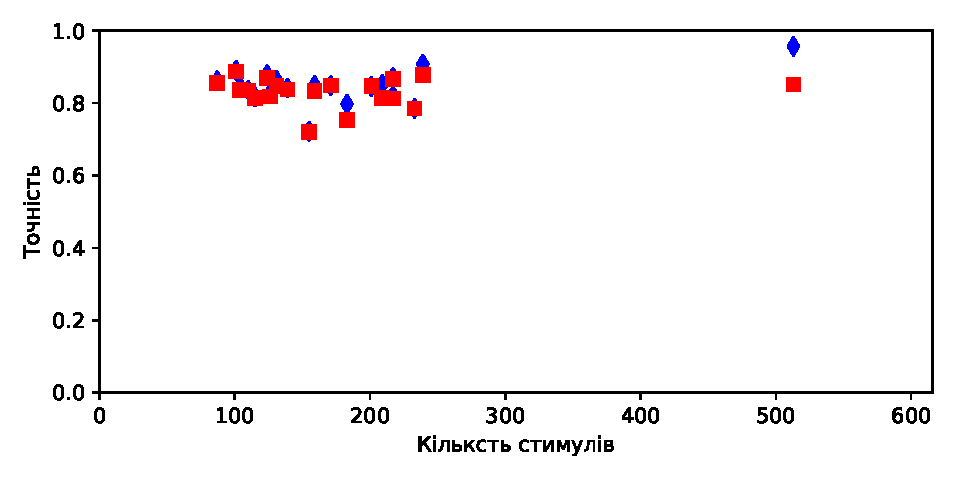
\includegraphics[width=.7\linewidth]{accuracy_distribution_data1_cnn}}
	\caption{Розподіл точності (червоні квадрати) та F-міри (сині ромби) за кількістю голосових зразків при моделюванні контекстів першого набору даних різними методами}
	\label{img:accuracy_distribution_data1}
\end{figure}
\begin{figure}[!t]
	\centering
	\subbottom[Метод ІРС розміром 1--3 \label{img:confusion_matrix_data1_irs13_context_21}]{%
		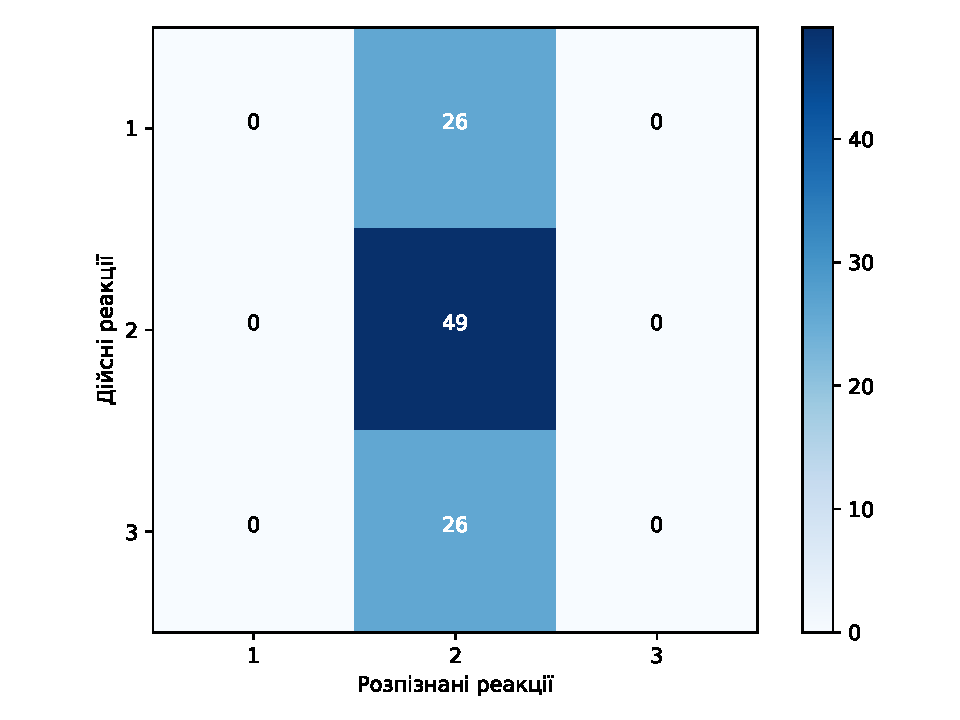
\includegraphics[width=0.3\linewidth]{confusion_matrix_data1_irs13_context_21}}
	\subbottom[Метод ІРС розміром 2--4 \label{img:confusion_matrix_data1_irs24_context_21}]{%
		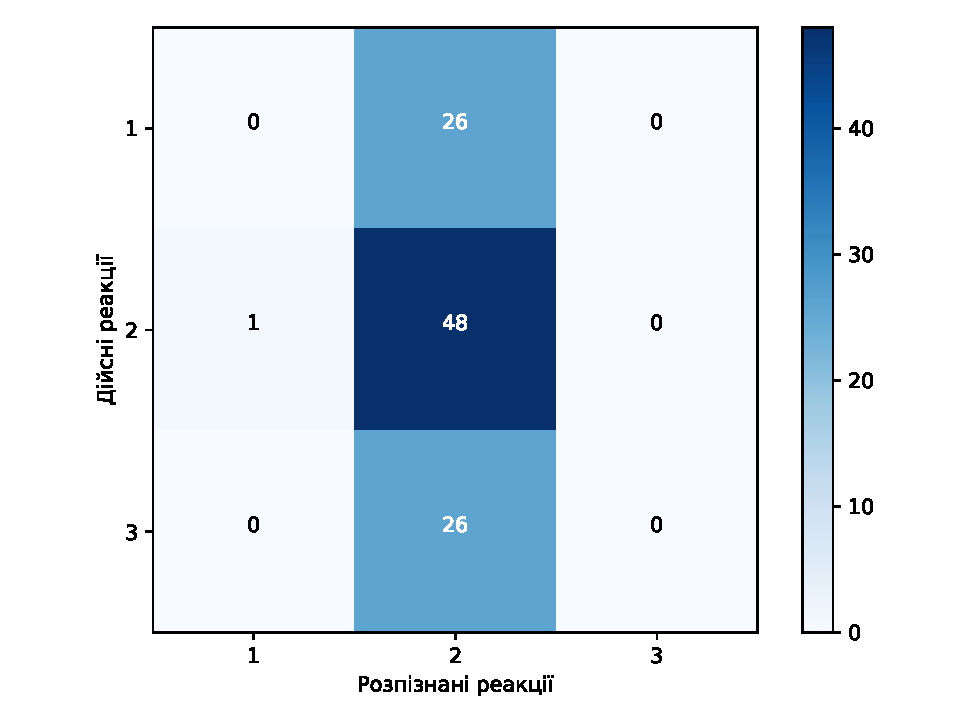
\includegraphics[width=0.3\linewidth]{confusion_matrix_data1_irs24_context_21}}
	\subbottom[Метод ЗНМ \label{img:confusion_matrix_data1_cnn_context_21}]{%
		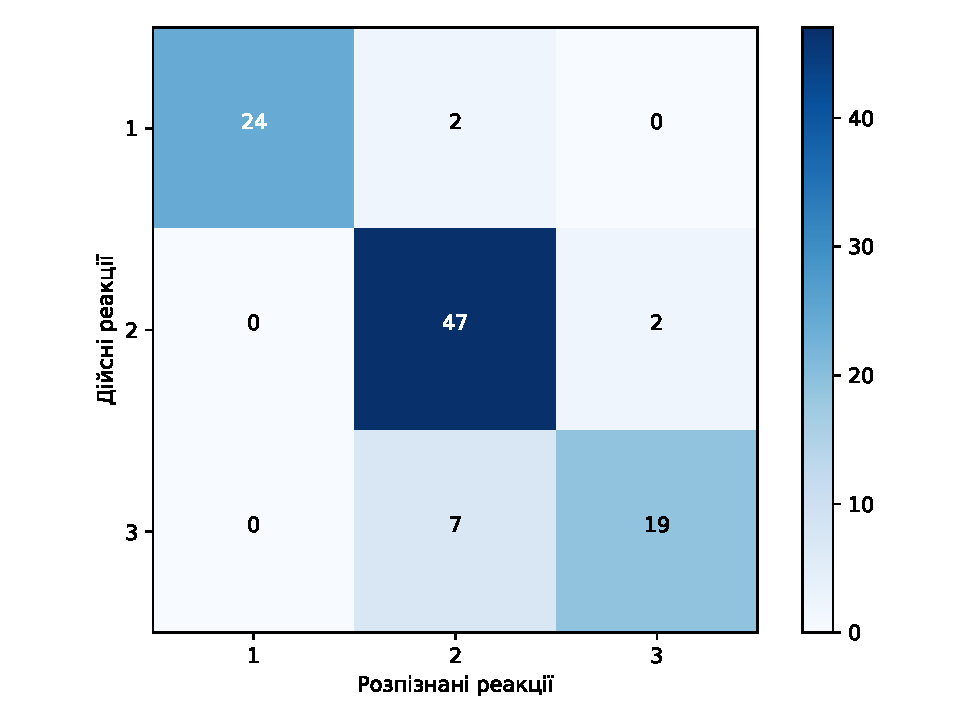
\includegraphics[width=0.3\linewidth]{confusion_matrix_data1_cnn_context_21}}
	
	\caption{Порівняння матриць помилок трьох різних методів (а, б, в) розпізнавання по реакціях для тестового контексту першого набору даних}
	\label{img:confusion_matrix_data1_context_21}
\end{figure}
\begin{mytable}{ | c | c | c | c | }%
	{Порівняння якості розпізнавання другого набору даних різними методами}%
	{\label{tbl:total_data2_irs13}}%
	{ Показник & ІРС 1--3 & ІРС 2--4 & ЗНМ }		
	
	Точність розпізнання & 0.258 & 0.598 & 0.935 \\
	\hline
	Середня прецизійність & 0.226 & 0.636 & 0.939 \\
	\hline
	Середня повнота & 0.238 & 0.579 & 0.935 \\
	\hline
	Середня F-міра & 0.217 & 0.583 & 0.937 \\
	\hline
	Кількість & 925 & 925 & 925 \\
\end{mytable}
\begin{figure}[ht!]
	\centering
	\subbottom[Метод ІРС розміром 1--3 \label{img:confusion_matrix_data2_irs13_context_21}]{%
		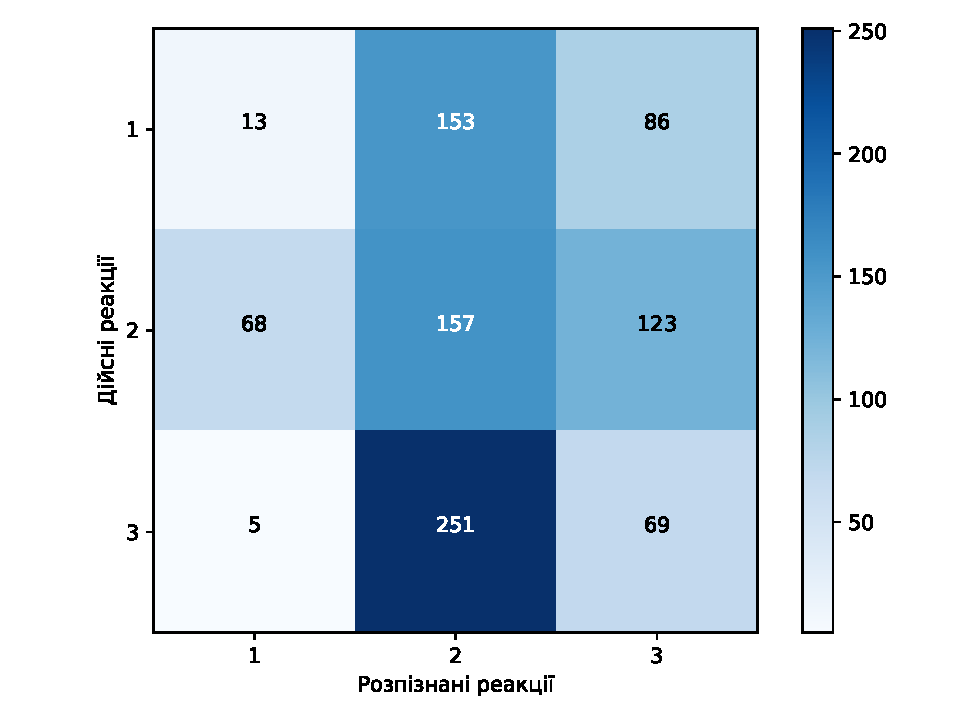
\includegraphics[width=0.3\linewidth]{confusion_matrix_data2_irs13_context_21}}
	\subbottom[Метод ІРС розміром 2--4 \label{img:confusion_matrix_data2_irs24_context_21}]{%
		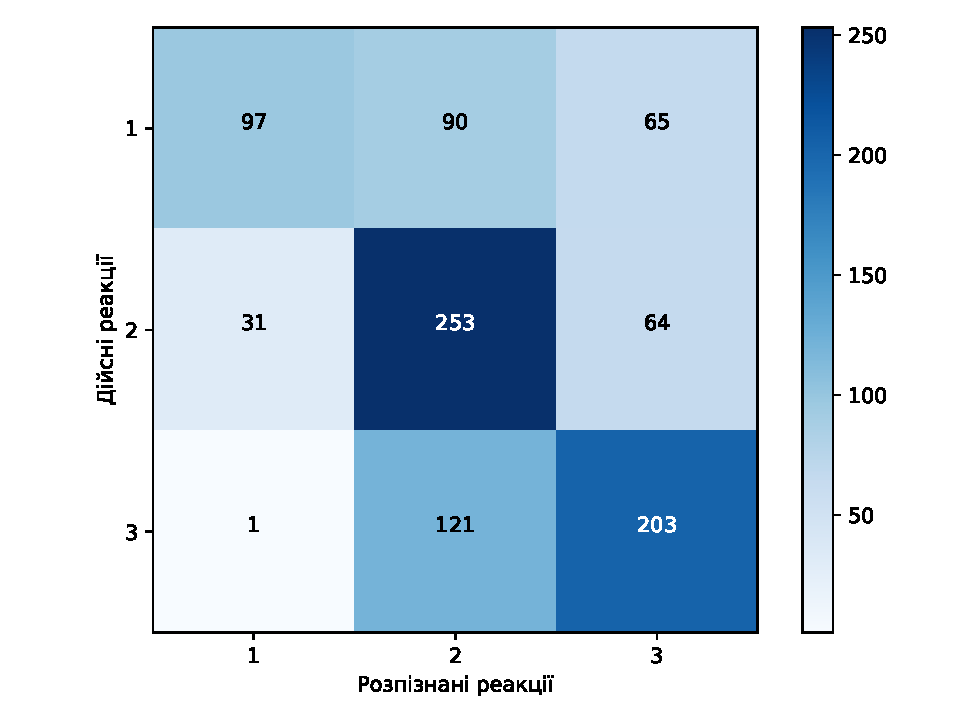
\includegraphics[width=0.3\linewidth]{confusion_matrix_data2_irs24_context_21}}
	\subbottom[Метод ЗНМ \label{img:confusion_matrix_data2_cnn_context_21}]{%
		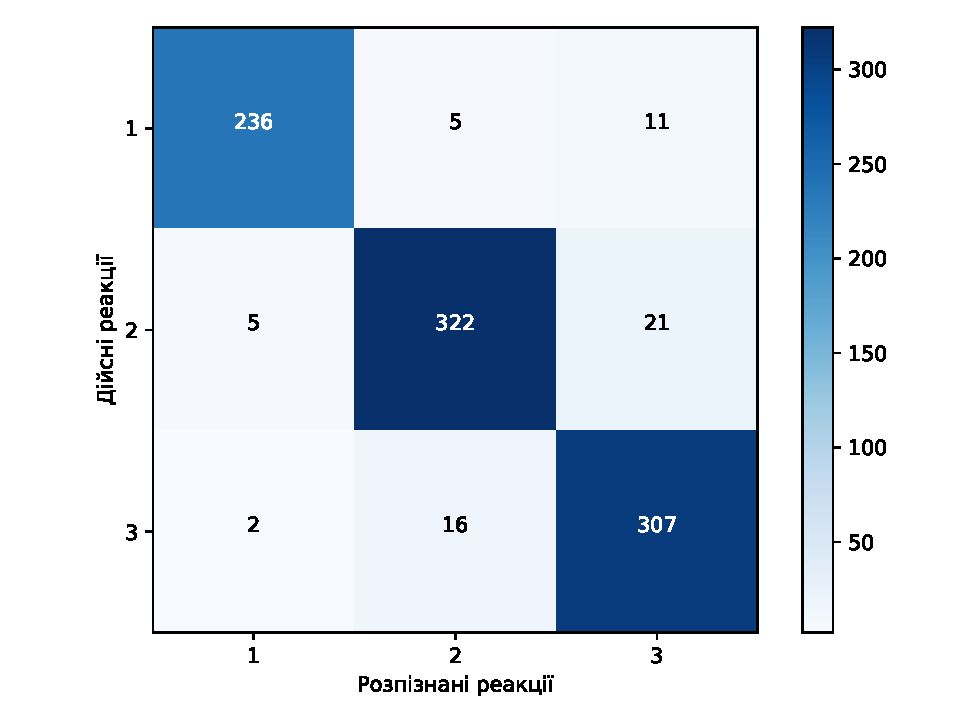
\includegraphics[width=0.3\linewidth]{confusion_matrix_data2_cnn_context_21}}
	
	\caption{Порівняння матриць помилок трьох різних методів (а, б, в) розпізнавання по реакціях для тестового контексту другого набору даних}
	\label{img:confusion_matrix_data2_context_21}
\end{figure}
\begin{mytable}[b!]{ | c | c | c | c | c | c | }%
	{Результати моделювання третього набору даних використовуючи ІРС з послідовностями розміром 1--3}%
	{\label{tbl:total_data3_irs13}}%
	{№ Контексту & \specialcell{3cm}{Точність \\ розпізнання} & \specialcell{3cm}{Середня \\ прецизійність} & \specialcell{3cm}{Середня \\ повнота} & \specialcell{3cm}{Середня \\ F-міра} & Кількість}	
	
	1 & 0.820 & 0.825 & 0.820 & 0.819 & 100 \\
\hline
3 & 0.637 & 0.660 & 0.637 & 0.611 & 350 \\
\hline
4 & 0.710 & 0.799 & 0.710 & 0.709 & 200 \\
\hline
5 & 0.630 & 0.714 & 0.630 & 0.633 & 300 \\
\hline
6 & 0.625 & 0.704 & 0.625 & 0.620 & 200 \\
\hline
7 & 0.524 & 0.563 & 0.524 & 0.528 & 500 \\
\hline
8 & 0.667 & 0.805 & 0.667 & 0.671 & 300 \\
\hline
9 & 0.660 & 0.790 & 0.660 & 0.667 & 250 \\
\hline
10 & 0.696 & 0.800 & 0.696 & 0.700 & 250 \\
\hline
11 & 0.608 & 0.703 & 0.608 & 0.600 & 250 \\
\hline
12 & 0.498 & 0.543 & 0.498 & 0.495 & 450 \\
\hline
13 & 0.700 & 0.697 & 0.700 & 0.698 & 150 \\
\hline
14 & 0.483 & 0.637 & 0.483 & 0.496 & 300 \\
\hline
15 & 0.597 & 0.664 & 0.597 & 0.587 & 300 \\
\hline
16 & 0.652 & 0.744 & 0.652 & 0.647 & 250 \\
\hline
17 & 0.431 & 0.495 & 0.431 & 0.430 & 350 \\
\hline
18 & 0.616 & 0.703 & 0.616 & 0.608 & 250 \\
\hline
19 & 0.595 & 0.713 & 0.595 & 0.596 & 200 \\
\hline
\specialcell{3cm}{По всій \\ вибірці} & 0.301 & 0.401 & 0.301 & 0.313 & 3200 \\
\hline
\specialcell{3cm}{Тестовий \\ контекст} & 0.733 & 0.738 & 0.733 & 0.734 & 150 \\
\end{mytable}
\begin{mytable}{ | c | c | c | c | c | c | }%
	{Результати моделювання третього набору даних використовуючи ІРС з послідовностями розміром 2--4}%
	{\label{tbl:total_data3_irs24}}%
	{№ Контексту & \specialcell{3cm}{Точність \\ розпізнання} & \specialcell{3cm}{Середня \\ прецизійність} & \specialcell{3cm}{Середня \\ повнота} & \specialcell{3cm}{Середня \\ F-міра} & Кількість}	
	
	1 & 0.850 & 0.616 & 0.567 & 0.590 & 100 \\
\hline
3 & 0.866 & 0.883 & 0.866 & 0.862 & 350 \\
\hline
4 & 0.870 & 0.898 & 0.870 & 0.867 & 200 \\
\hline
5 & 0.830 & 0.863 & 0.830 & 0.830 & 300 \\
\hline
6 & 0.835 & 0.876 & 0.835 & 0.829 & 200 \\
\hline
7 & 0.774 & 0.795 & 0.774 & 0.775 & 500 \\
\hline
8 & 0.857 & 0.882 & 0.857 & 0.851 & 300 \\
\hline
9 & 0.884 & 0.763 & 0.737 & 0.737 & 250 \\
\hline
10 & 0.864 & 0.895 & 0.864 & 0.865 & 250 \\
\hline
11 & 0.824 & 0.852 & 0.824 & 0.814 & 250 \\
\hline
12 & 0.751 & 0.780 & 0.751 & 0.753 & 450 \\
\hline
13 & 0.813 & 0.655 & 0.610 & 0.620 & 150 \\
\hline
14 & 0.730 & 0.788 & 0.730 & 0.734 & 300 \\
\hline
15 & 0.780 & 0.824 & 0.780 & 0.778 & 300 \\
\hline
16 & 0.840 & 0.865 & 0.840 & 0.832 & 250 \\
\hline
17 & 0.646 & 0.692 & 0.646 & 0.641 & 350 \\
\hline
18 & 0.740 & 0.803 & 0.740 & 0.739 & 250 \\
\hline
19 & 0.825 & 0.853 & 0.825 & 0.821 & 200 \\
\hline
\specialcell{3cm}{По всій \\ вибірці} & 0.637 & 0.676 & 0.627 & 0.628 & 3200 \\
\hline
\specialcell{3cm}{Тестовий \\ контекст} & 0.893 & 0.895 & 0.893 & 0.894 & 150 \\
\end{mytable}
\begin{mytable}{ | c | c | c | c | c | c | }%
	{Результати моделювання третього набору даних використовуючи ЗНМ з послідовностями розміром 2--4}%
	{\label{tbl:total_data3_cnn}}%
	{№ Контексту & \specialcell{3cm}{Точність \\ розпізнання} & \specialcell{3cm}{Середня \\ прецизійність} & \specialcell{3cm}{Середня \\ повнота} & \specialcell{3cm}{Середня \\ F-міра} & Кількість}	
	
	1 & 0.900 & 0.901 & 0.900 & 0.900 & 100 \\
\hline
3 & 0.997 & 0.997 & 0.997 & 0.997 & 350 \\
\hline
4 & 0.990 & 0.990 & 0.990 & 0.990 & 200 \\
\hline
5 & 0.967 & 0.967 & 0.967 & 0.966 & 300 \\
\hline
6 & 0.975 & 0.976 & 0.975 & 0.975 & 200 \\
\hline
7 & 0.948 & 0.950 & 0.948 & 0.948 & 500 \\
\hline
8 & 0.983 & 0.984 & 0.983 & 0.983 & 300 \\
\hline
9 & 0.976 & 0.976 & 0.976 & 0.976 & 250 \\
\hline
10 & 0.960 & 0.961 & 0.960 & 0.960 & 250 \\
\hline
11 & 0.952 & 0.956 & 0.952 & 0.951 & 250 \\
\hline
12 & 0.951 & 0.952 & 0.951 & 0.950 & 450 \\
\hline
13 & 0.927 & 0.926 & 0.927 & 0.926 & 150 \\
\hline
14 & 0.950 & 0.950 & 0.950 & 0.950 & 300 \\
\hline
15 & 0.923 & 0.925 & 0.923 & 0.922 & 300 \\
\hline
16 & 0.968 & 0.971 & 0.968 & 0.968 & 250 \\
\hline
17 & 0.951 & 0.954 & 0.951 & 0.952 & 350 \\
\hline
18 & 0.928 & 0.929 & 0.928 & 0.928 & 250 \\
\hline
19 & 0.980 & 0.981 & 0.980 & 0.980 & 200 \\
\hline
\specialcell{3cm}{По всій \\ вибірці} & 0.890 & 0.891 & 0.890 & 0.890 & 3200 \\
\hline
\specialcell{3cm}{Тестовий \\ контекст} & 0.973 & 0.974 & 0.973 & 0.973 & 150 \\
\end{mytable}
\begin{figure}[!t]
	\centering
	\subbottom[Метод ІРС розміром 1--3 \label{img:accuracy_distribution_data3_irs13}]{%
		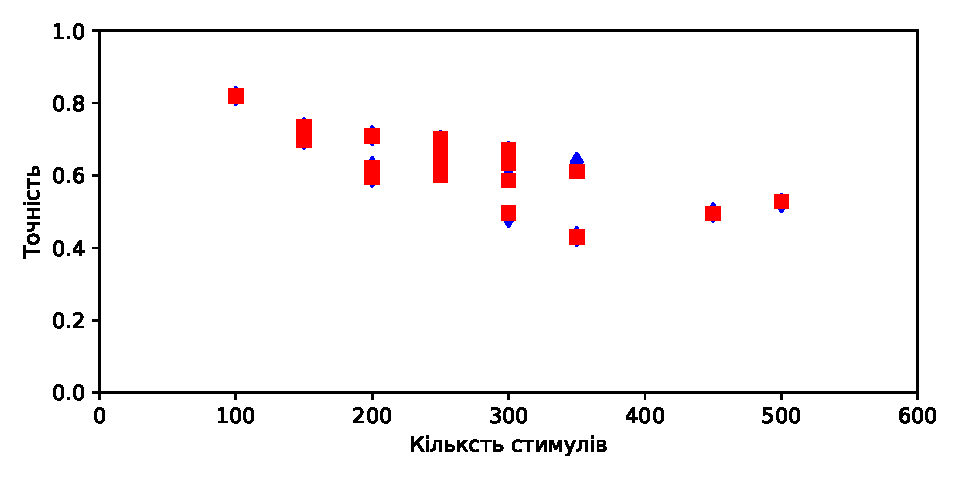
\includegraphics[width=.7\linewidth]{accuracy_distribution_data3_irs13}}
	\\
	\subbottom[Метод ІРС розміром 2--4 \label{img:accuracy_distribution_data3_irs24}]{%
		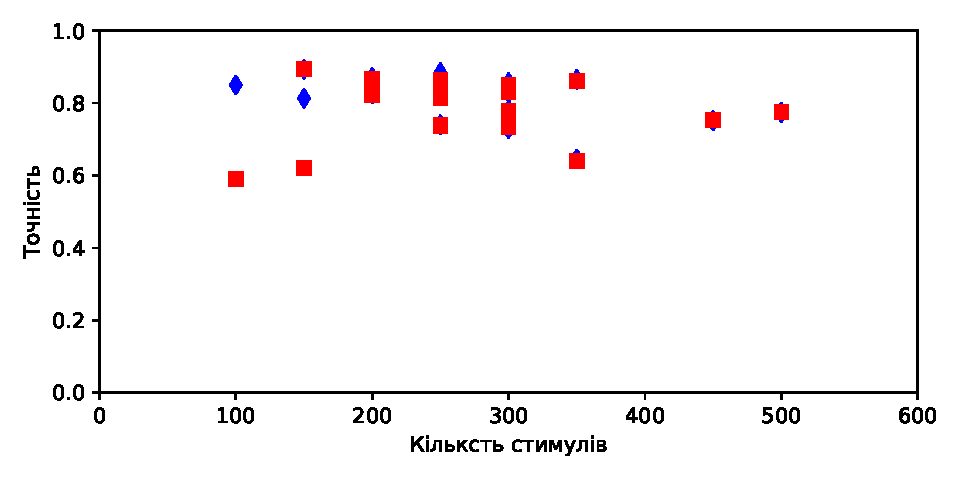
\includegraphics[width=.7\linewidth]{accuracy_distribution_data3_irs24}}
	\\
	\subbottom[Метод ЗНМ \label{img:accuracy_distribution_data3_cnn}]{%
		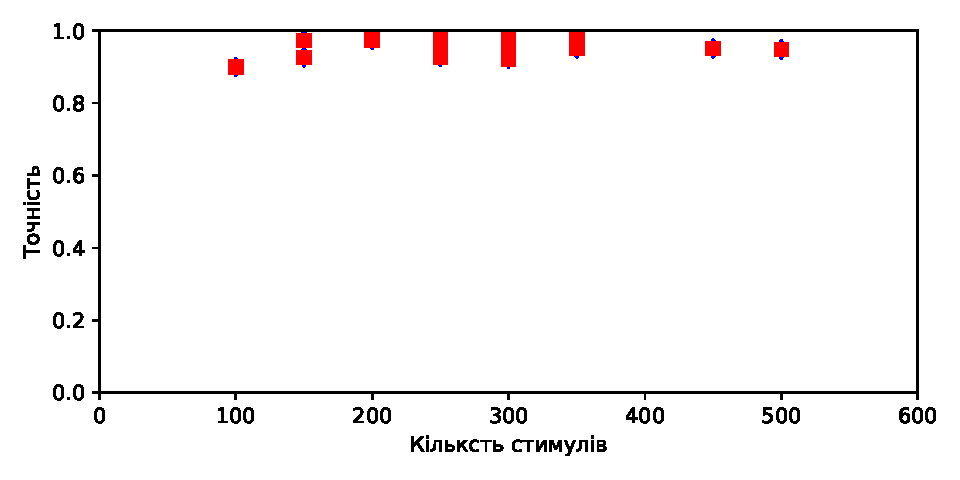
\includegraphics[width=.7\linewidth]{accuracy_distribution_data3_cnn}}
	\caption{Розподіл точності (червоні квадрати) та F-міри (сині ромби) за кількістю голосових зразків при моделюванні контекстів третього набору даних різними методами}
	\label{img:accuracy_distribution_data3}
\end{figure}
\begin{figure}
	\centering
	\subbottom[Метод ІРС розміром 1--3 \label{img:confusion_matrix_data3_irs13_context_21}]{%
		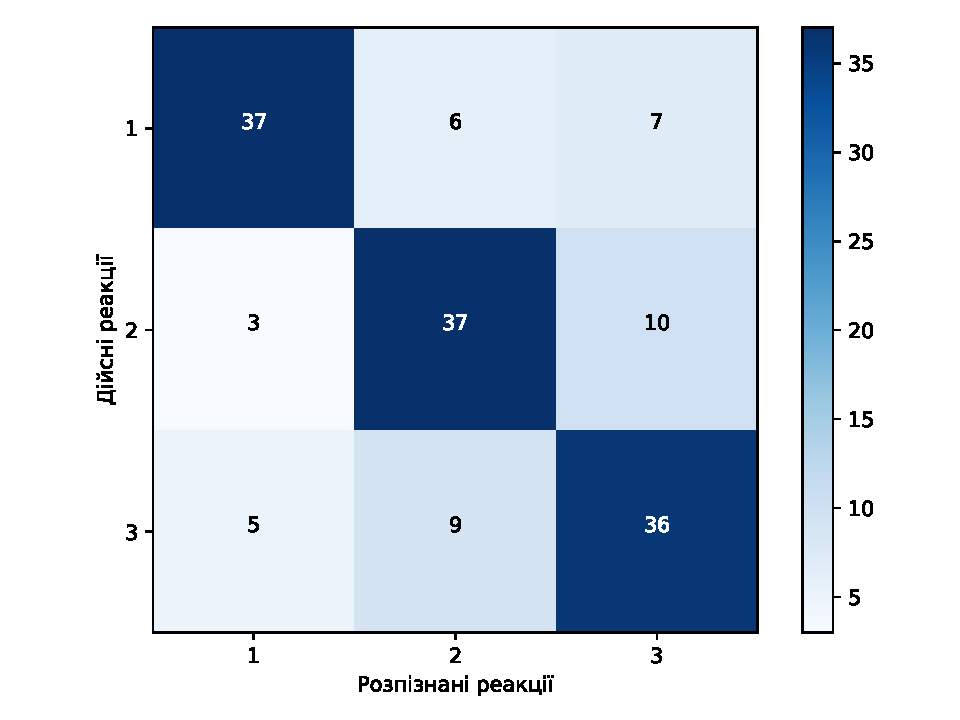
\includegraphics[width=0.3\linewidth]{confusion_matrix_data3_irs13_context_21}}
	\subbottom[Метод ІРС розміром 2--4 \label{img:confusion_matrix_data3_irs24_context_21}]{%
		\includegraphics[width=0.3\linewidth]{confusion_matrix_data3_irs24_context_21}}
	\subbottom[Метод ЗНМ \label{img:confusion_matrix_data3_cnn_context_21}]{%
		\includegraphics[width=0.3\linewidth]{confusion_matrix_data3_cnn_context_21}}
	
	\caption{Порівняння матриць помилок трьох різних методів розпізнавання по реакціях для тестового контексту третього набору даних}
	\label{img:confusion_matrix_data3_context_21}
\end{figure}
